% \documentclass[12pt]{book}
\documentclass[12pt,openany]{book} % openany option allows chapters to start not just on odd pages (so gets rid of blank pages)
\usepackage{color}
%\usepackage{colortbl}
\usepackage{hyperref}
\usepackage{graphicx}
\usepackage{fancyhdr}
\usepackage{version}
\usepackage{wrapfig}
%\usepackage[all,dark]{draftcopy}
\usepackage{type1cm} % watermark
\usepackage{eso-pic} % watermark

\excludeversion{COMMENT}


\pagestyle{fancy}
%\pagestyle{headings}

\setlength{\oddsidemargin}{0.0in}
\setlength{\evensidemargin}{0.0in}
\setlength{\topmargin}{-0.0in}
\setlength{\headheight}{0.0in}
\setlength{\textwidth}{6.5in}
\setlength{\textheight}{8.5in}
\setlength{\headwidth}{\textwidth}

\newcommand{\bkorel}[1]{\textcolor{red}{bkorel: {#1}}}
\newcommand{\cjenkins}[1]{\textbf{\textcolor{blue}{cjenkins: {#1}}}}
\newcommand{\hilight}[1]{\colorbox{yellow}{#1}}


\makeatletter
\AddToShipoutPicture{%
            \setlength{\@tempdimb}{.5\paperwidth}%
            \setlength{\@tempdimc}{.5\paperheight}%
            \setlength{\unitlength}{1pt}%
            \put(\strip@pt\@tempdimb,\strip@pt\@tempdimc){%
        \makebox(0,0){\rotatebox{45}{\textcolor[gray]{0.75}%
        {\fontsize{6cm}{6cm}\selectfont{DRAFT}}}}%
            }%
}
\makeatother

\title{Teaching Autonomous Robotics Using Player and ROS: \\ A CS 148 Starter Guide (DRAFT)}
\author{Barbara Teresa Korel \hspace{1cm} Odest Chadwicke Jenkins}

\begin{document}

\maketitle

% % \title{Teaching Autonomous Mobile Robotics using Player and ROS}
% % \date{Spring 2010}
% % \author{Jenkins\\ Korel\\ Crick\\}
% % \maketitle
% % \newpage

% preamble distinguishing this draft from final book

\chapter*{Foreword}

This draft contains the first three chapters of the developing textbook ``Teaching Autonomous Robotics Using Player and ROS''.  This draft satisfies the project requirements for Barbara Korel towards the completion of her Masters degree in Computer Science at Brown University, under the supervision of Prof. Chad Jenkins.  This book is based on the development and experiences restructuring an undergraduate robotics course, Brown University CS 148 ``Building Intelligent Robots'', for the iRobot Create platform.  Chad Jenkins has taught this updated version of CS 148 since 2006, with Barbara Korel serving as Head Teaching Assistant in 2009.

This draft is intended to serve as a ``how-to'' guide to setup a basic low-cost mobile robot platform for use in an upper-level undergraduate robotics course.  Subsequent chapters will cover project modules suitable for courses using the described robot platform.  The projects will cover bug and random navigation algorithms, color object recognition, path planning, robot localization, subsumption architectures, multi-robot coordination, learning from demonstration, and experimentation with significance testing.  Up-to-date developments for these materials can be found from the CS 148 website (http://www.cs.brown.edu/courses/cs148) and the Brown Robotics code repository (http://code.google.com/p/brown-rlab/).

\begin{titlepage}

\begin{center}
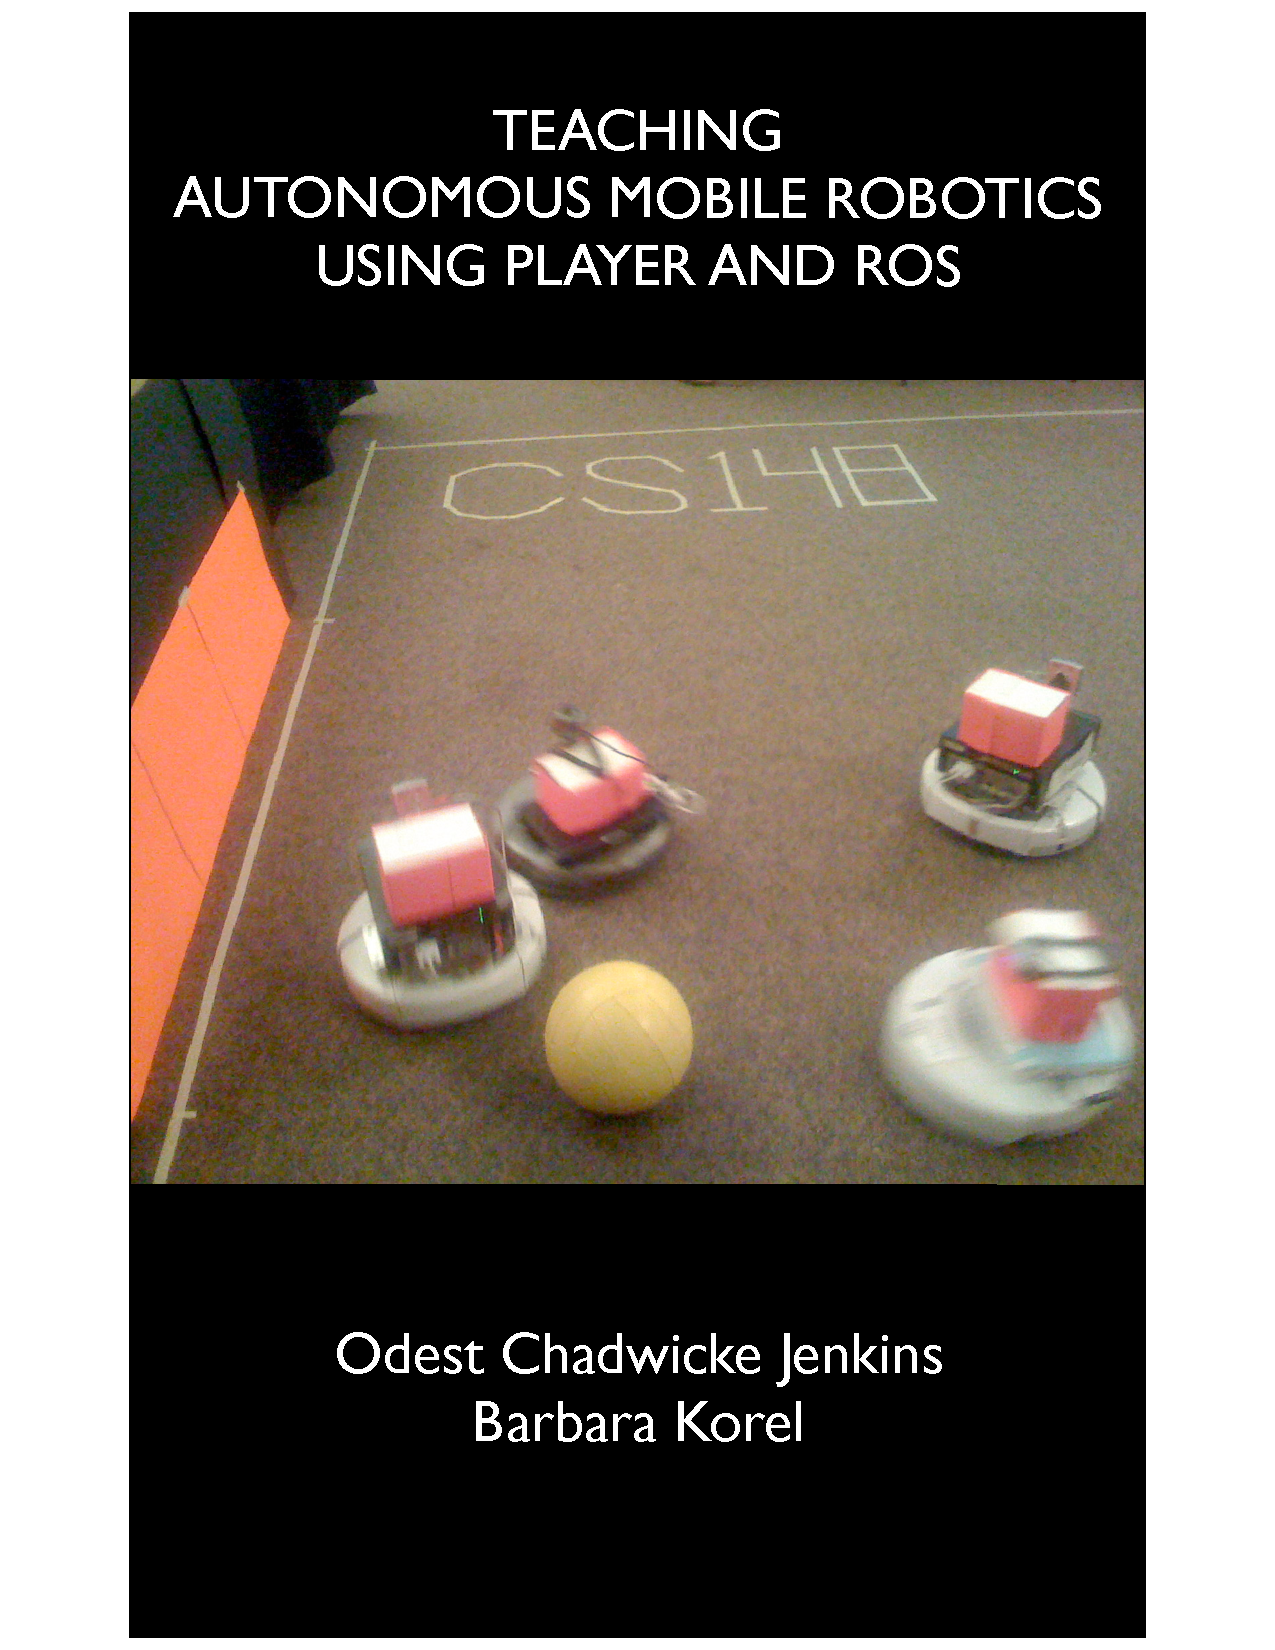
\includegraphics[scale=0.76]{figures/book_cover_may2010.pdf}
%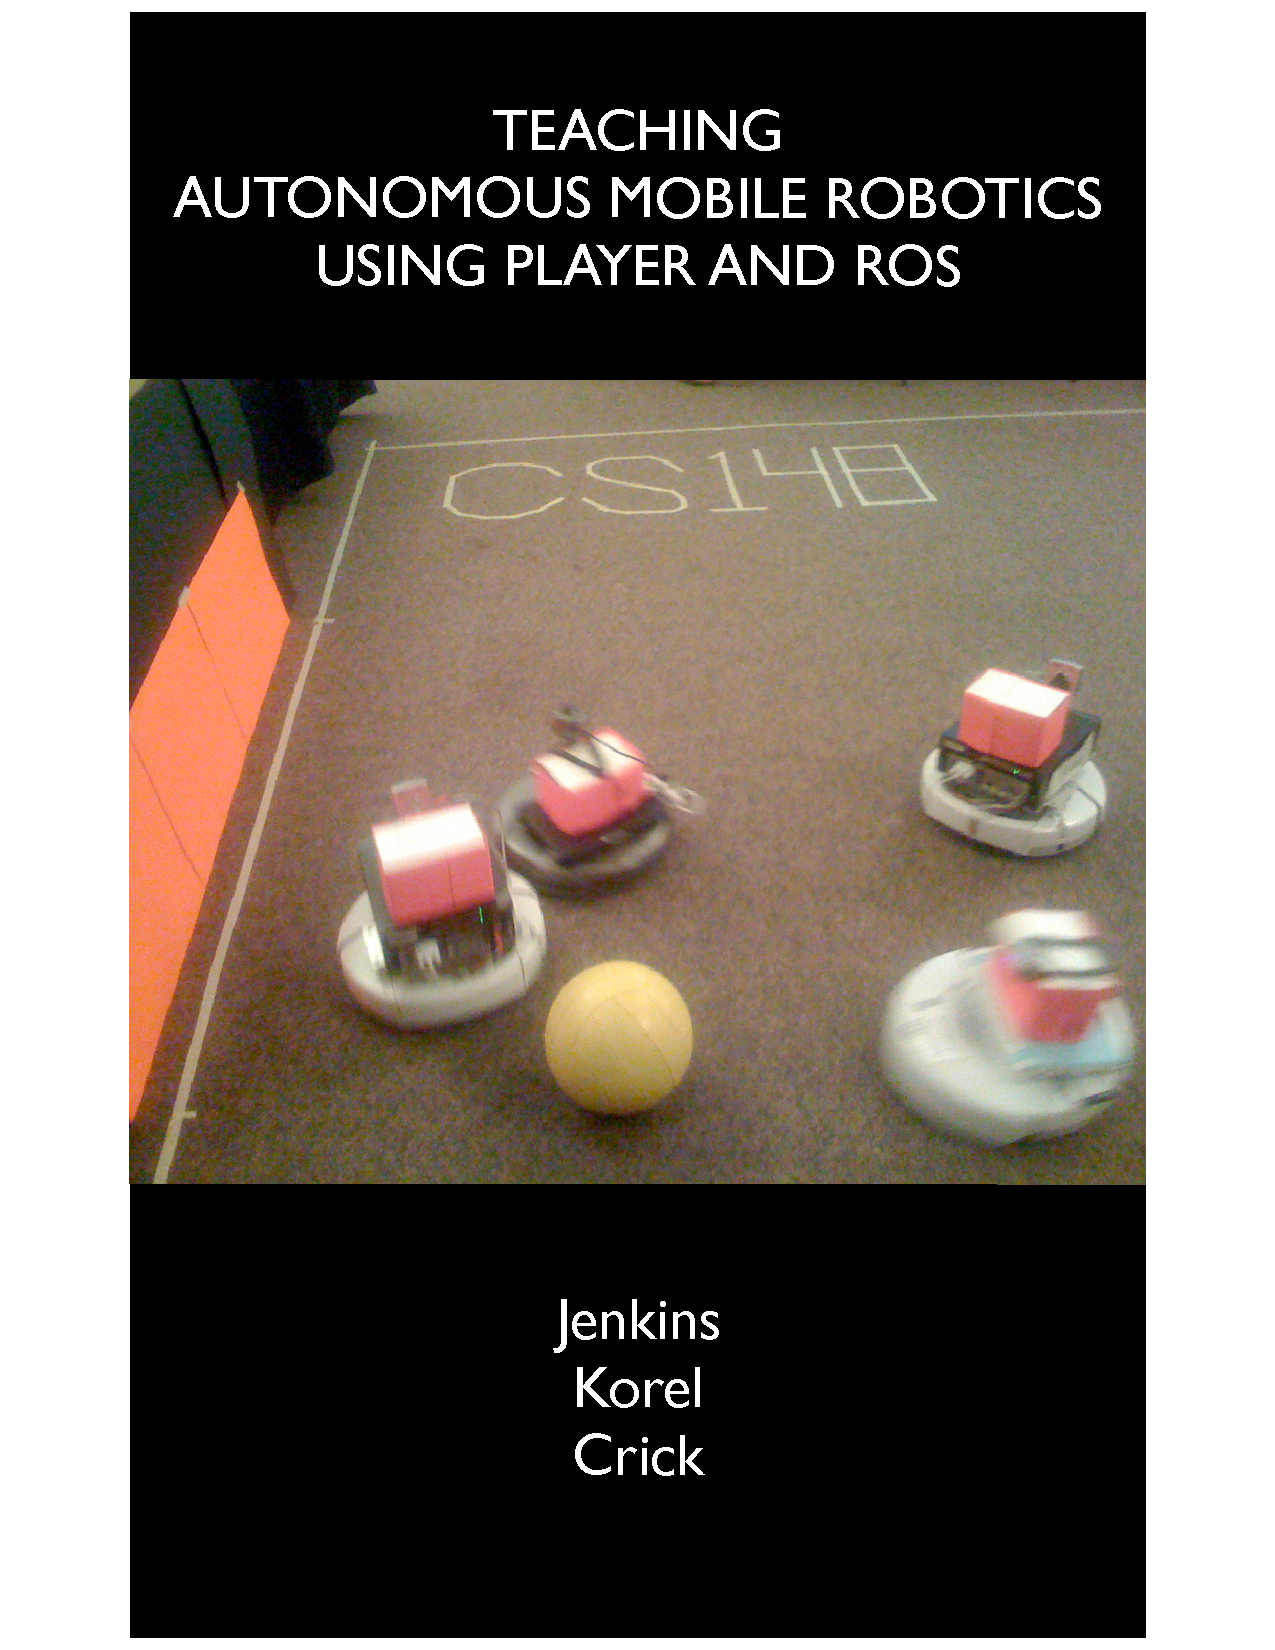
\includegraphics[scale=0.76]{figures/book_cover.pdf}
\end{center}

\end{titlepage}

\lhead{Teaching Autonomous Robotics with Player and ROS  }

\tableofcontents
\newpage

\rhead{Course Objectives}

\chapter{Course Objectives}

\begin{figure}[!h]
\centering
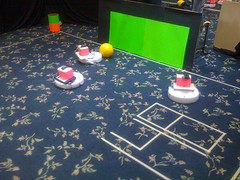
\includegraphics[width=0.8\columnwidth]{figures/1_teaser.jpg}
\end{figure}

\newpage

\begin{wrapfigure}{r}{0.35\columnwidth}
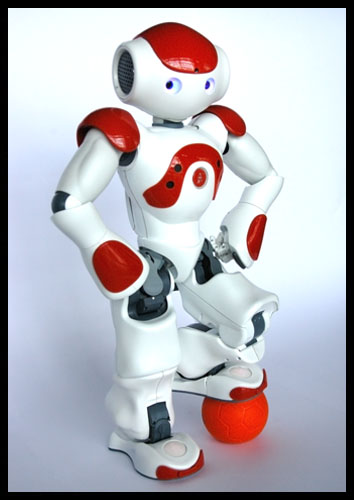
\includegraphics[width=0.3\columnwidth]{figures/1_Nao.jpg}
\caption{The Aldebaran Nao.}
\label{fig:1_Nao}
\end{wrapfigure}

This book is based on our experiences developing and restructuring an undergraduate robotics course, Brown University CS 148 ``Building Intelligent Robots'', for the iRobot Create platform.  Taking the perspective of CS 148, we describe our objectives and approach for an upper-level course in autonomous robotics.  Our main educational goal is to focus on the computational aspects of robotics while minimizing the necessary mechatronic startup costs, which is best suited for a complementary course.  To this end, we use a solderless robot platform comprised of ``off-the-shelf'' components that can be readily assembled by undergraduate (and secondary) students.  This platform is meant to be both a quick entry point for students to start programming robots and, using research-grade robot middleware (e.g., Player, ROS), a path that can directly lead to understanding and extending the state-of-the-art in robotics.

For instructors, this book is meant to be a ``how-to'' guide for getting an autonomous robotics course modules up-and-running with as little overhead as possible.  The first three chapters describe how to assemble, program and remotely control a basic low-cost mobile robot platform.  Subsequent chapters cover project modules suitable for this (and similar) mobile robotics, as conducted in CS 148 in recent years.  These projects build upon each other from bug and random navigation algorithms and color object recognition up through path planning, robot localization, subsumption architectures, multi-robot coordination, learning from demonstration, and experimentation with significance testing.  These projects are pedagogically cast within a ``robot control loop'' (consisting of sensing, perception, decision making, motion control, and physics).  The control loop serves as a conceptual scaffold similar to the notion of a pipeline in computer graphics. 

In terms of collaboration, this book is intended to be a community resource that facilitates sharing and collaboration in and beyond the classroom.  Given the larger integrative nature of robotics projects, CS 148 projects utilize version control systems (Subversion in particular) to enable collaboration among student groups, reproducibility by course graders, and portability when moving code across robots.  For educators, this book itself and supporting materials will be maintained (and continually updated) in a Subversion repository:

\begin{verbatim}
   http://brown-rlab.googlecode.com/svn/trunk/teaching_autonomous_robotics
\end{verbatim}

We encourage educators to freely use the book and materials in their courses and broader educational efforts.  These materials are meant to be copy-pasted, modified, tested, and refined as a community to improve the quality and accessibility of robotics education.  We welcome and encourage contributions to the continued development of this book, especially those that can be patched into the repository.  Up-to-date usage of these materials in CS 148 can be accessed through the course website:

\begin{verbatim}
   http://www.cs.brown.edu/courses/cs148
\end{verbatim}



\section{CS 148 Course Description}

\texttt{(taken from Brown 2009-10 course catalog)}

CS148 is an introduction to fundamental topics in autonomous robot control. This course focuses on the development of ``brains'' for robots. That is, given a machine with sensing, actuation, and computation, how do we develop programs that allow the machine to function autonomously? We answer this question through a series of class discussions and group projects.

CS148 class meetings cover technical and algorithmic aspects of robotic decision making and perception, as well as societal and philosophical implications posed by autonomous robots. Discussions amongst the class pose and address questions related to how robots can contribute to society, what technical functionality is needed, and how will such technologies affect the human-robot dynamic.

CS148 projects center on a ``robot soccer'' task, where students program robot vacuum-like devices to play soccer in a structured environment. Various approaches to robot control (spanning reaction to deliberation) are covered using the \href{http://robotics.cs.brown.edu/projects/smurv/}{Brown iRobot Create platform robots} (which are \href{http://www.irobot.com/sp.cfm?pageid=122}{iRobot Roomba/Create} hardware with onboard ASUS EeePC subnotebooks, as seen in Figure \ref{fig:1_create_platform} on the far right). We support either the \href{http://playerstage.sourceforge.net}{Player/Stage/Gazebo (PSG)} robot framework or the \href{http://www.ros.org/wiki/ROS/StartGuide}{Robot Operating System (ROS)} as a robot middleware solution for the course projects. Similarly, the project implementations are not restricted to the iRobot Create platforms. Rather any robot that has the physical components for playing soccer, such as Aldebaran's \href{http://www.aldebaran-robotics.com/eng/Nao.php}{Nao humanoid robot} (Figure \ref{fig:1_Nao}), can be used to program the assignments. Thus, the practical aspects of this course are not limited to a specific robot platform or middleware. 

\begin{figure}[!h]
\centerline{
\mbox{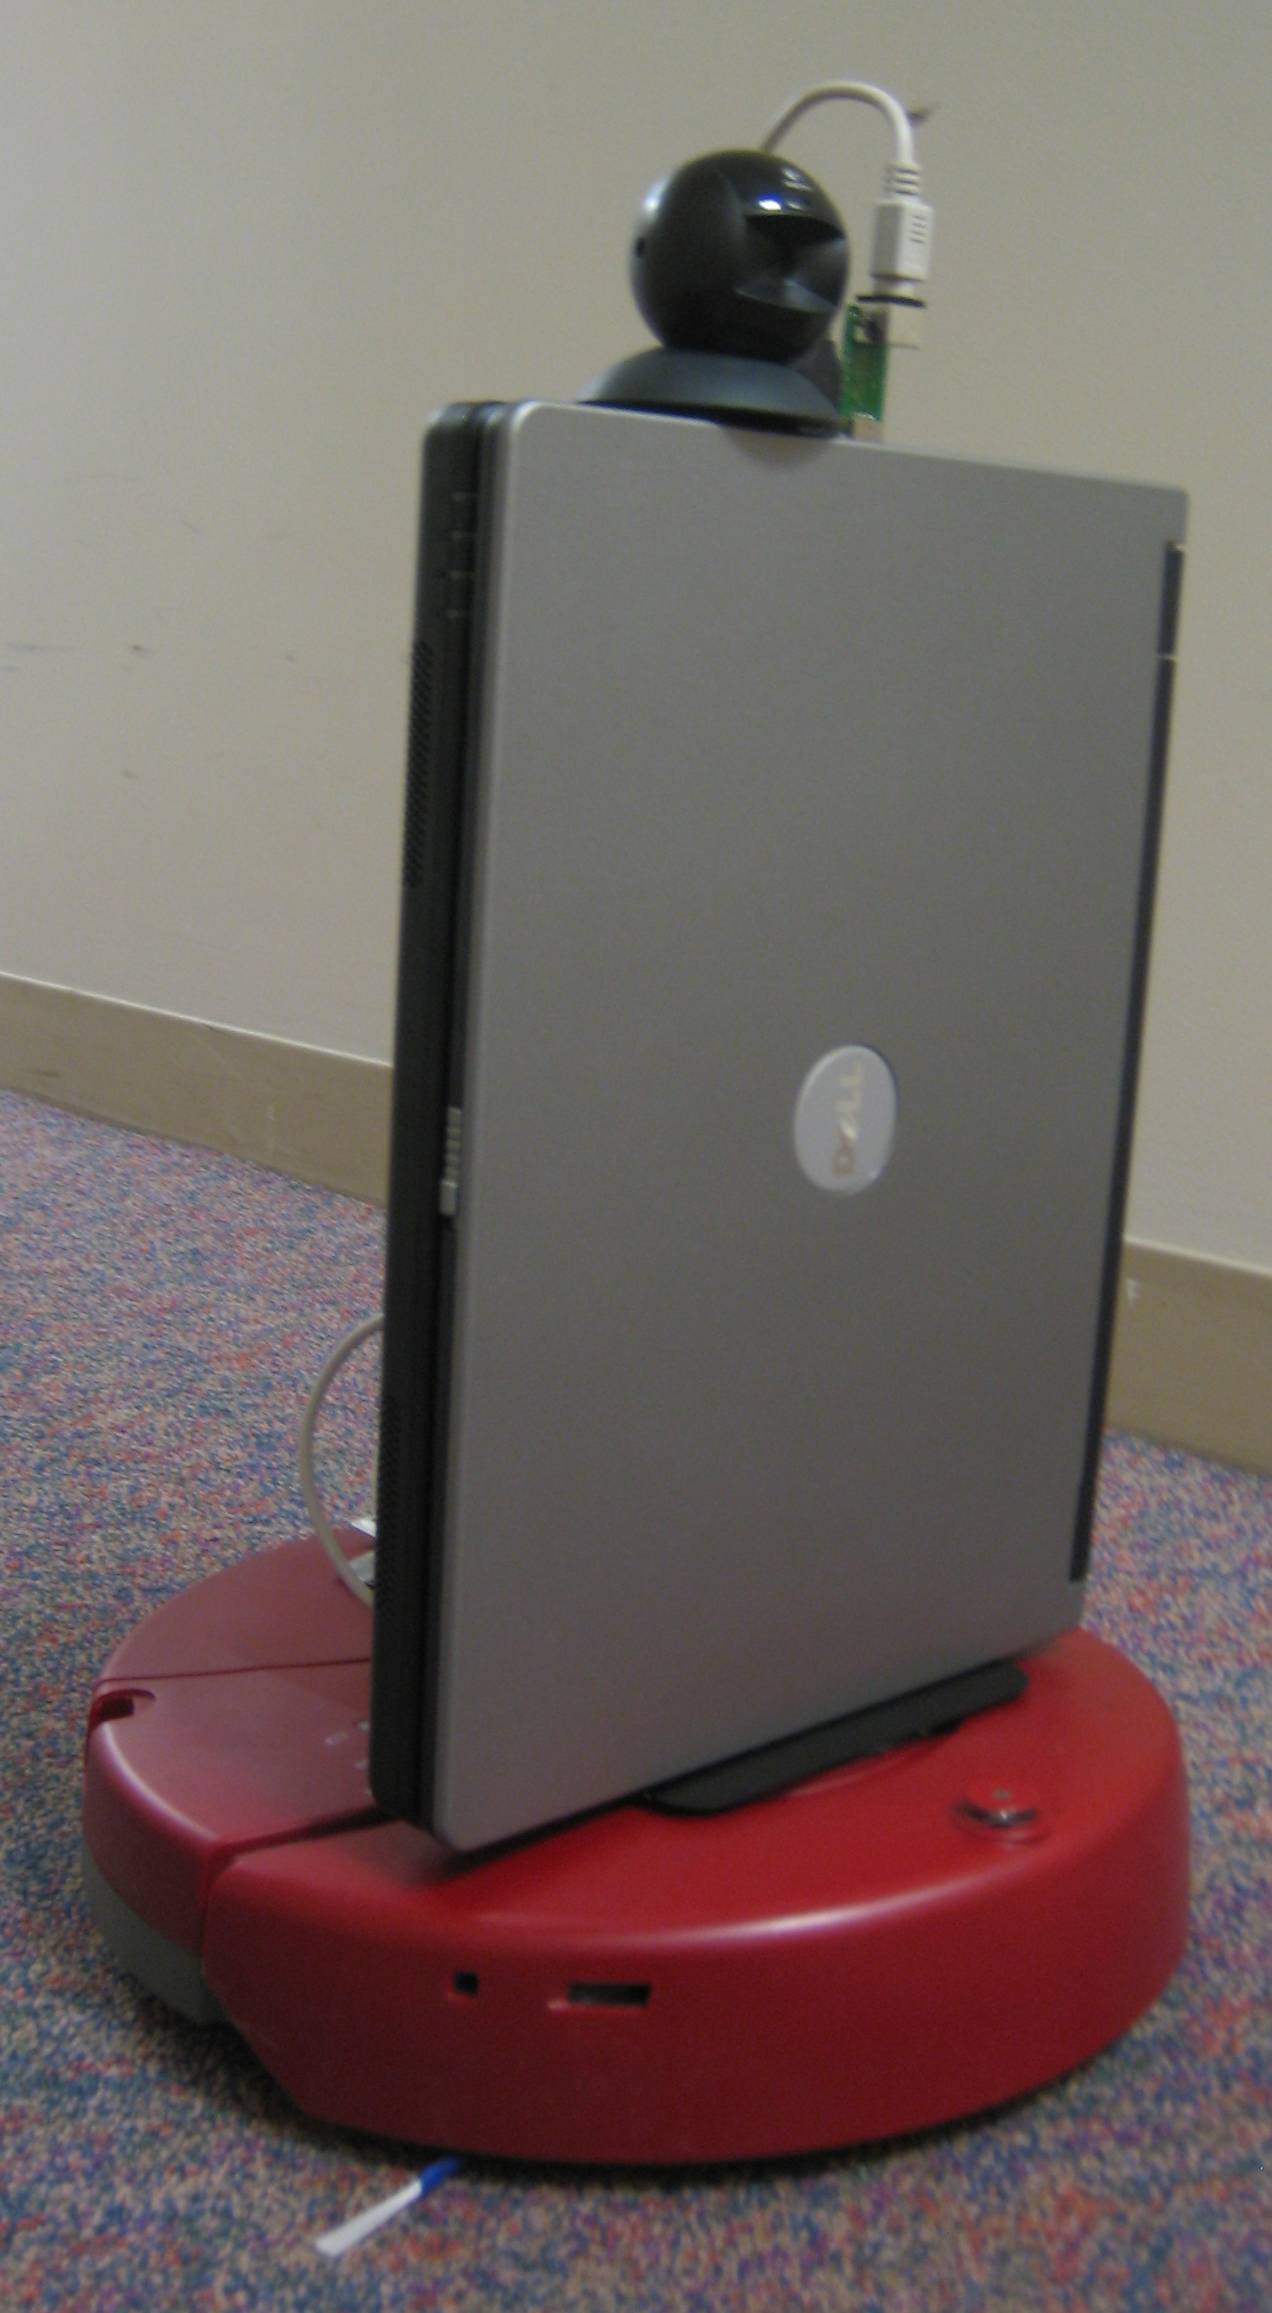
\includegraphics[height=1.6in]{figures/1_platformv1.png}}
\mbox{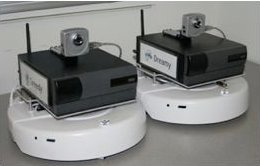
\includegraphics[height=1.6in]{figures/1_create_platformv1.jpg}}
\mbox{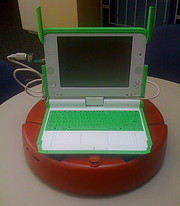
\includegraphics[height=1.6in]{figures/1_create_v2.jpg}}
\mbox{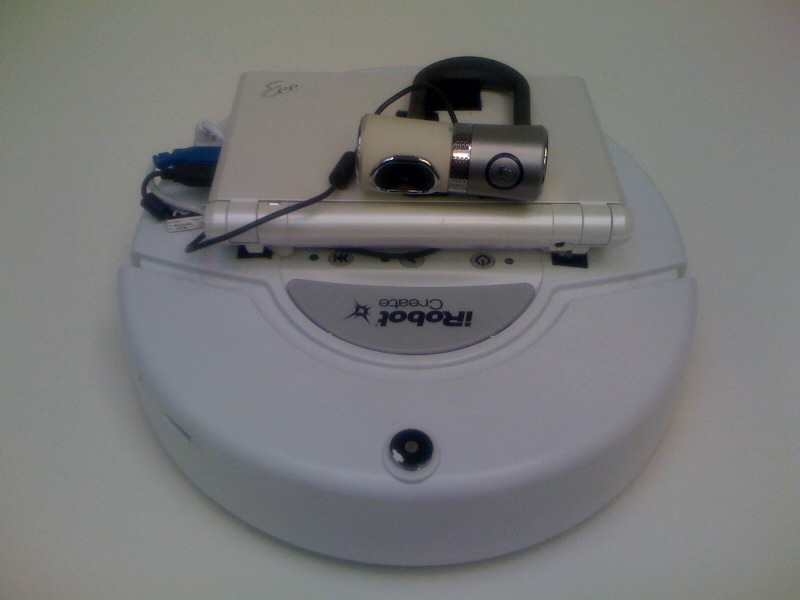
\includegraphics[height=1.6in]{figures/1_create_platform.jpg}}
}
\caption{Evolution of the Brown SmURV robot platform. Version 0.5 (2006), Logitech QuickCam and iRobot Roomba connected to a larger Dell laptop, usually carried offboard, using a RoboDynamics RooStick.  Version 1.0 (2007), a Mini-ITX computer and Unibrain Fire-I camera connected to and powered by an iRobot Create.  Version 1.5 (2008), a One Laptop Per Child XO, with onboard camera, connected to a Roomba.  Version 2.0 (2009), an Asus EEE PC and Logitech QuickCam Ultra on an iRobot Create. }
\label{fig:1_create_platform}
\end{figure}

%%\bkorel{picture of PS3 cam with newer laptop and create?)

\section{Why Robotics?}

Why should anyone consider robotics?  One quick answer: the 3 D's, ``Dirty, Dull, and Dangerous.''  Robots have long been proposed as a way to relieve humans from tasks necessary for society that can be unpleasant, mundane, or hazardous to human health.  More generally, robotics can be considered a means to enhance physical human productivity that augments or even multiplies a human user's ability to perform tasks in the physical world.

The application of robots already has a strong presence in many different fields, illustrated in the collage of Figure \ref{fig:1_robotic_applications}.  In healthcare, robots have assisted doctors, nurses, and caretakers in the delivery of medicines in hospitals, surgical operations, and post-stroke rehabilitation.  The use of robotics has the potential to reduce health care costs and help the elderly and chronically ill to remain independent. Exploration robots have been able to collect scientific data on planets and deep sea areas that would be difficult (perhaps impossible) for humans to reach.  Domestic service robots such as the iRobot Roomba and Willow Garage's PR2 can perform basic household chores, such as vacuuming and laundry.  Robots in manufacturing assist with labor intensive jobs to lower production costs and increase productivity.  Unmanned vehicles for military applications, such as the General Atomics MQ-1 Predator and iRobot PackBot, can provide greater reconnaissance and reduce the risk of human casualties by using robots in place of humans.  Along with the benefits of each of these applications, robots raise serious questions about unintended or harmful consequences, such as the effects to world labor markets and global armed conflicts.

\begin{figure}[!h]
\centering
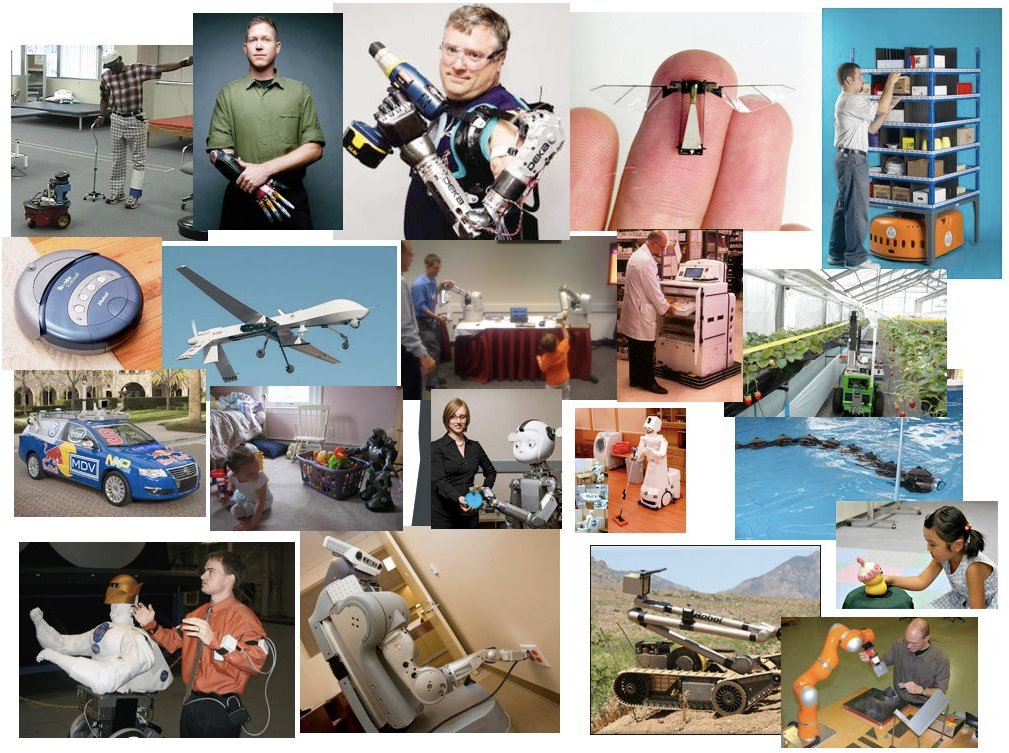
\includegraphics[width=0.7\textwidth]{figures/1_robotic_applications.jpg}
\caption{Examples of robotic applications.}
\label{fig:1_robotic_applications}
\end{figure}

Given this wide array of applications, it is important to note that robotics is not necessarily about to replace human labor.  Although not currently the case, at some point, robots may outperform humans at certain jobs due to being cheaper, faster, or easier to train.  However, robots will not and should not be the right solution for all of society's labor.  Rather, robotics should complement human productivity. There are many tasks that will remain difficult for robots, such as those that involve intuition, uncertainty, or human sociability.  The most productive use of robots will likely specialize robotic tasks to those that are not necessarily suited to or desired by their human users.  For example, instead of spending an hour vacuuming their house, a human user can delegate this task to a robot and spend this hour exercising.

\begin{figure}[!h]
\centering
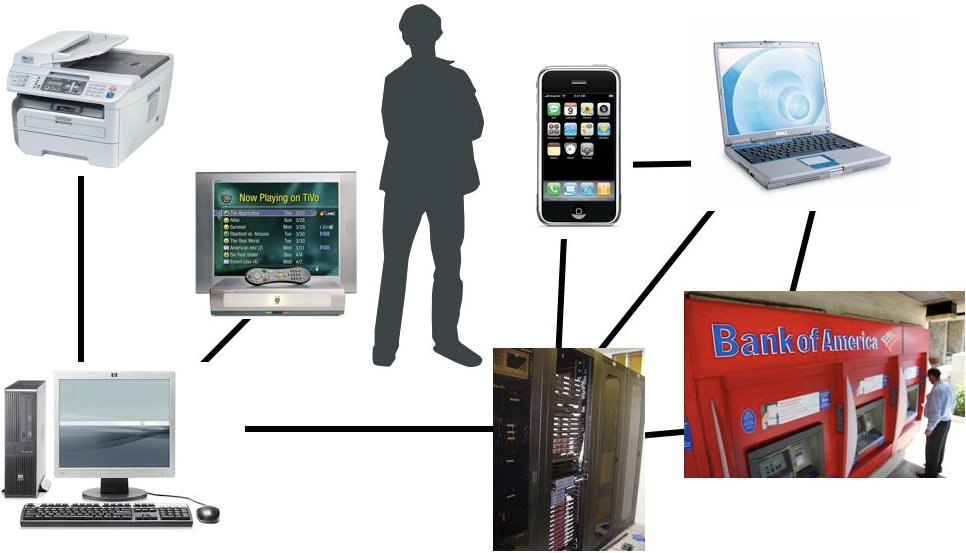
\includegraphics[width=0.7\textwidth]{figures/1_personal_computing.jpg}
\caption{Examples of heterogeneous computing devices.}
\label{fig:1_personal_computing}
\end{figure}

%\cjenkins{add note about many heterogenous devices for a single individual}

Robotics can also be thought of as an extension of computing and the Internet beyond digital worlds into the physical world that we inhabit. The explosion of personal computing devices present in our everyday lives, as seen in Figure \ref{fig:1_personal_computing}, have become not just an amenity but a necessity. Personal computing has enabled individuals to significantly increase their productivity in digital domains, such as electronic communication, publishing, and virtual telepresence (teleconferencing, video games, etc.).  Similarly, the prevalence of commodity robotic devices will move this productivity past the digital boundary and into the physical world. 

\begin{figure}[!h]
\centering
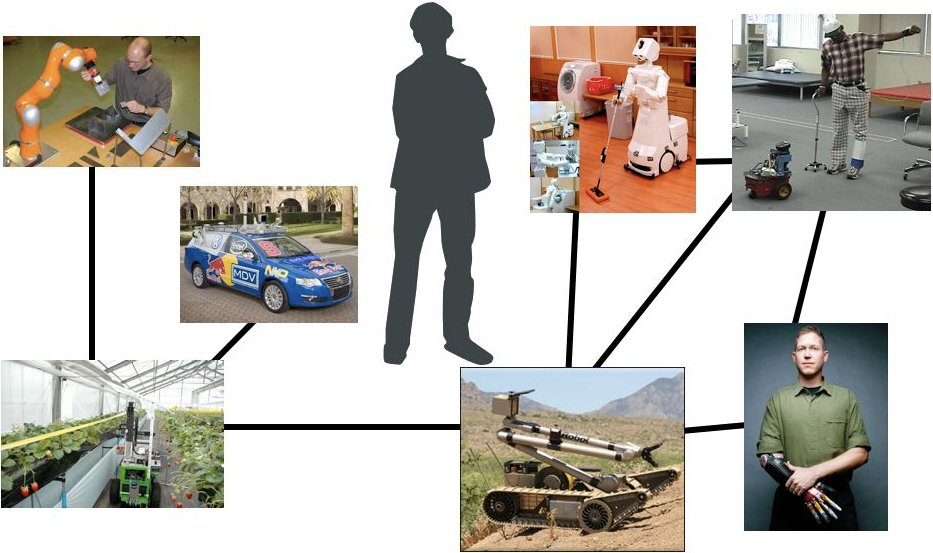
\includegraphics[width=0.7\textwidth]{figures/1_robot_apps.jpg}
\caption{Examples of heterogeneous robotic devices.}
\label{fig:1_robot_apps}
\end{figure}

Finally, whereas personal computing has enabled individuals to manage digital information by supervising teams of heterogeneous computing devices, autonomous robotics will enable individuals to manage physical environments by supervising teams of heterogeneous robotic devices, as seen in Figure \ref{fig:1_robot_apps}. If a heterogeneous collection of robots is to affect the physical world by interacting with and manipulating its features to achieve a predefined desire, the coordination among the robotic devices is essential. The question of how to coordinate and control a team of heterogeneous robotic devices is still an open challenge and needs to be addressed for this vision to be realized. 

\subsection{The Personal Robotics Revolution}

\begin{figure}[!h]
\centering
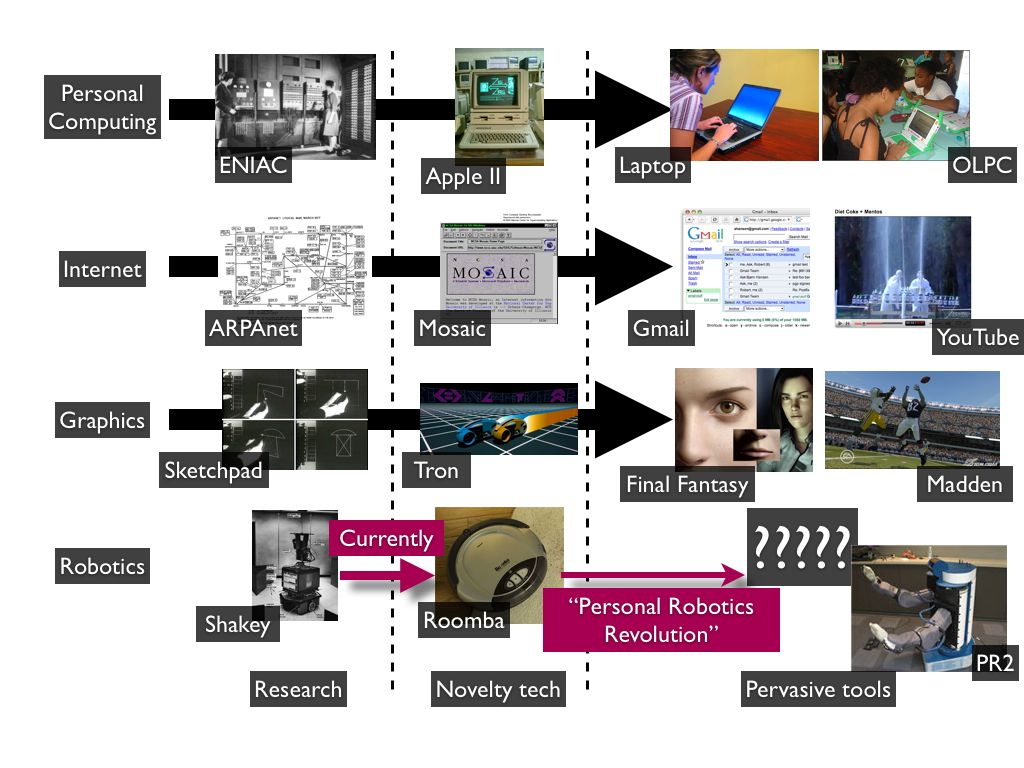
\includegraphics[width=0.85\textwidth]{figures/1_revolution.jpg}
\end{figure}

While problematic, the challenges of the physical world offer new and great opportunities for the pioneering spirit.  Think of robotics as a means to extend computing and the Internet beyond controlling digital environments into autonomously working in the physical world.  This is the perfect time to be a roboticist because innovators can shape the technology!  Similar to the ``personal computing revolution'' a few decades ago, robotics is on the dawn of its own \href{http://fora.tv/2009/05/30/Rodney\_Brooks\_Remaking\_Manufacturing\_With\_Robotics}{``personal robotics revolution''}, with many great robotic technologies that are now starting to come together. 

Robotics is currently in the same stage of the exponential technology growth as personal computing in the 1970s, computer graphics in the 1980s and the Internet in the early 1990s.  These three trends all hit the technology exponential, explained by Moore's law which describes ``a long-term trend in history of computing hardware, in which the number of transistors that can be placed inexpensively on an integrated circuit has doubled approximately every two years."\footnote{\href{http://en.wikipedia.org/wiki/Moore\%27s_law}{Moore's law: en.wikipedia.org/wiki/Moore\%27s\_law}}. Robotics is currently a technology exponential in the making, thus this is the time to get involved in robotics!

\subsection{CS 148 Disclaimer: the real world is unforgiving}

\begin{wrapfigure}{l}{0.35\columnwidth}
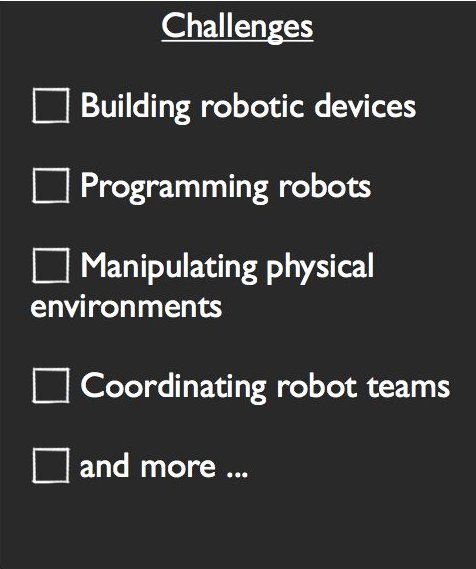
\includegraphics[width=0.3\columnwidth]{figures/1_challenges.jpg}
\end{wrapfigure}

The first prerequisite for building intelligent robots is to engineer robotic devices. Provided the abundance of robot systems along with the commercial availability of relatively cheap robots such as the Roomba, for the purposes of this class we will assume this prerequisite has been successfully met. The next challenge is to program robots to function autonomously in an unpredictable world. This is the challenge CS148 will address.

This course involves a significant amount of programming and decision making under uncertainty. Robotics is about understanding and functioning in the real world. However, the real world is highly dynamic, uncontrolled, and nondeterministic. These factors result in uncertainty that is unlike the structure and determinism of traditional computer science. Programming in the face of such uncertainty is a persistent challenge faced at all levels of robotics. Keep in mind that robots are not sentient, but their programmers are!


\section{Autonomous Robotics}

%Autonomy means an independence of control. In robotics this refers to the ability of a robot to perform desired tasks by making decisions and acting on them without any human intervention. 

We define an autonomous robot as a decision making agent with a physical embodiment that acts solely based on its perception of the world through sensors and its own internal information.  Teleoperated robots, or robots that are controlled by human operators, are not autonomous and are not studied in this course. Because humans are not directly making decisions for the robot, an autonomous control program must be executed that performs the ``cognitive'' functions of the robot, specifically: perception, decision making, and executing actions (or motion control). Combined these components act as the brains for the robot and enable the robot to be autonomous. 

CS148 is the study of autonomous robotics. That is, given robot hardware with sensing and actuation, we are challenged with programming the robot to autonomously perform a task. The algorithms and architectures for autonomous robot control are studied, which provide the ability to perceive, make decisions and act. It is important to note that this course is not a robotics engineering course. We will not build robot hardware, nor study in detail the physical dynamics and kinematics for expressing motion or robot control theory. CS148 utilizes a relatively cheap robot platform that allows us to study both in theory and in practice the core concepts of autonomous control.

\subsection{Robot Control Loop}

\begin{figure}[!h]
\centering
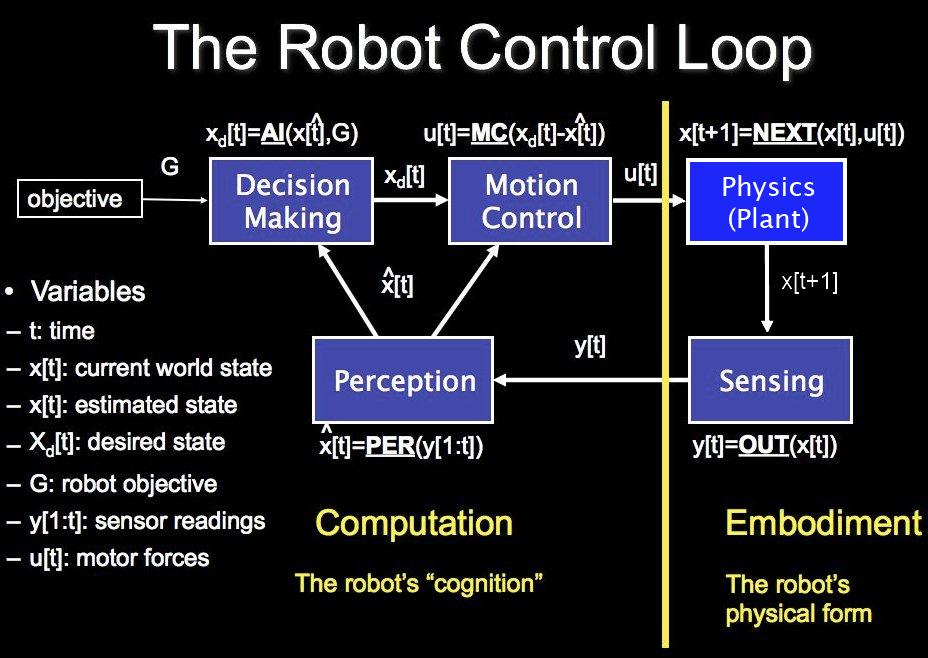
\includegraphics[width=0.85\textwidth]{figures/1_control_loop_white.png}
\label{fig:1_control_loop}
\end{figure}

The functions of all autonomous robots can be cast into a robot control loop. The robot control loop must be examined under the five main components that constitute an autonomous robot: plant, sensors, perception, decision making, and movement (or motion control.

The physical embodiment of the robot and its dynamics with the world is called the \textit{plant}.  The plant, or robot platform, allows a robot to exist in the physical world and interact with other physical objects in its environment. The plant is the physical embodiment and is subject to the same laws of physics that apply to humans and any other object. The plant consists of the body of the robot, including motors and actuators; it is the material structure that is the robot's presence in the world.

The robot's \textit{sensing} is its observations about the current state of the world. The information the robot collects through its sensors serves as input for perceiving the environment's state.  Sensing does not provide a complete view of the world, but is rather partial observations from the robot's perspective.  
%The sensors are not to be confused with sensing; sensors are the hardware on the plant that actually receives data whereas sensing is the process of collecting information about itself and the current state of the world.

The \textit{perception} component of the control loop uses the readings gathered from sensing and perceives the information in terms of itself and the environment to estimate, to the best of its abilities, the current state of the world.

Because we would like to have our robots perform some function, every robot must have an ``objective'' or goal. The overall goal of a robot may have different levels of abstraction and the overall goal may consist of many sub-goals; however only one objective can serve as the input to the control loop during a single iteration. An autonomous robot uses both the perceived state of the world and an object to guide the \textit{decision making} component of the control loop. Decision making determines the next action the robot should take.

Finally, in order to change the state of the physical embodiment, robots must have \textit{motion control}, based on perception and decision making that dictates the next state of the robot in terms of its physical parts. The motion control calculates the control forces that should be applied to the actuators in order for the robot to enact the desired action.

Together the plant and sensors compose the ``embodiment'' of the robot: the physical body and a mechanism of sensing to gather information about the environment. CS148 does not cover in substance topics within robot engineering for building the embodiment (actuators, sensors, physical parts) of a robot. For robots that are teleoperated or explicitly programmed to perform a specific task without ``thinking'', our discussion of the robot control loop can end here; our robot would just consist of the embodiment. 
%However, this course is really interested in exploring what makes a robot autonomous and how can we solve the next problem using autonomous robots. Thus 
In contrast, CS148 focuses on the autonomous, or ``cognitive'', aspects of this loop, pertaining to programming procedures for perception (state estimation), decision making (deciding how to act), and motion control (executing decided actions).

Lectures and activities in CS148 are centered around the basic notion of an autonomous robot control loop, as illustrated in Figure \ref{fig:1_control_loop}. The algorithms that we study are cast as components in this loop that will be used to form complete project implementations. 

\section{Course Format}

Topics covered during lectures will be grounded implementations during interactive sessions and 7 assignments.  Interactive sessions are devoted to a hands-on introduction to Player/Stage/Gazebo, ROS, Matlab, and working with our iRobot Create platforms leading up to the projects.

\subsection{Assignments}

The first three assignments are introductions to basic issues defining autonomous robotics and implementing robot controllers using either the Player or ROS robot middleware:

\begin{figure*}
\centerline{
\mbox{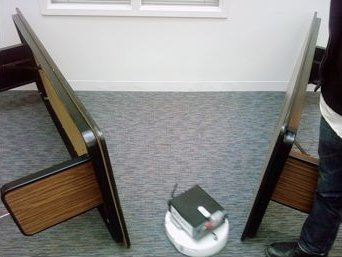
\includegraphics[width=2.01in]{figures/1_enclosure.jpg}}
\mbox{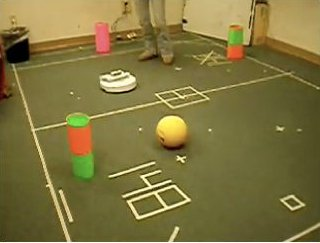
\includegraphics[width=1.99in]{figures/1_objrec.jpg}}
\mbox{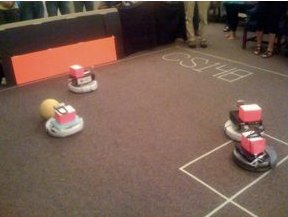
\includegraphics[width=2.0in]{figures/1_multi.jpg}}
}
\caption{Projects: Enclosure Escape, Object Recognition and Multi-robot Coordination.}
\end{figure*}

\begin{itemize}
\item Ch \ref{sec:create_spotting} Create Spotting: run experiments and analyze two built-in behaviors on the iRobot Create bases.
\item Ch \ref{sec:enclosure_escape} Enclosure Escape: implement a reactive random traversal robot control policy to escape from an enclosure.
\item Ch \ref{sec:object_seeking} Object Seeking: implement a control policy to continually seek and visit two objects in alternation.
\end{itemize}

The remaining projects explore different approaches to autonomous robot control in the context of robot soccer with various constraints on sensing and using heterogeneous robot hardware:

\begin{figure}[!h]
\centering
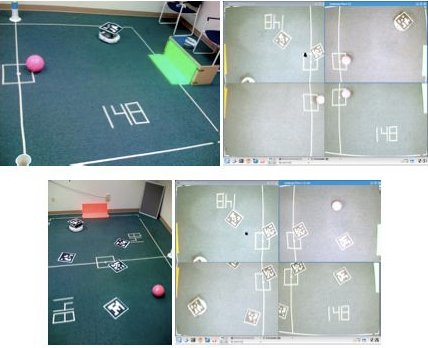
\includegraphics[width=0.6\textwidth]{figures/1_planning.jpg}
\caption{Path Planning Project.}
\end{figure}

\begin{itemize}
\item Ch \ref{sec:path_planning} Path Planning: given a map of the field and an overhead camera view of the environment, develop a deliberative planning-based robot client for visiting specific locations and pushing a ball into a goal.
\item Ch \ref{sec:localization} Monte Carlo Localization (MCL): same objective as path planning, except the camera view is onboard the moving robot.
\item Ch \ref{sec:subsumption} Subsumption: develop a goal scoring controller without maintaining any state (history or timing variables).
\item Ch \ref{sec:multi_robot} Multi-Robot Coordination: given a team of one SmURV/Create and one unknown robot platform, develop a competitive multi-robot strategy and individual controllers.
\item Ch \ref{sec:learning}  Learning: guide a fixed learning algorithm to play a control policy without explicit programming.
\end{itemize}

\subsection{Robot Soccer}

The CS148 projects all center around developing controllers to play robot soccer.  Robot soccer has been an active topic of research for over a decade.  RoboCup is the worldwide effort to advance the state of the art in robot soccer through yearly competitions.  Their goal is to field a team of robot soccer players capable of winning against the human World Cup champion by 2050 (Kitano).

\begin{figure*}
\centerline{
\mbox{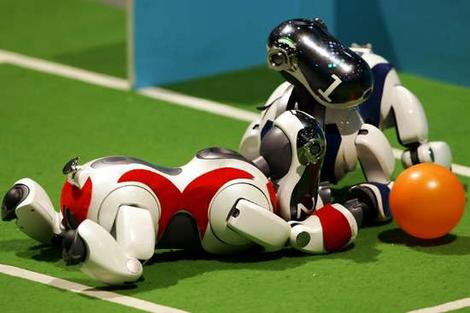
\includegraphics[width=2.98in]{figures/1_robocup06.jpg}}
\mbox{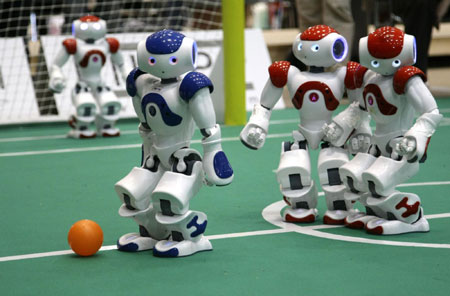
\includegraphics[width=3.00in]{figures/1_robocup09.jpg}}
}
\caption{4-legged League (RoboCup 2006); Standard Platform League (RoboCup 2009).}
\end{figure*}

This class considers a constrained version of this problem using the low-cost Brown iRobot Create platform and a highly structured soccer environment.  The robots programmed for the course projects will likely not outplay any humans or RoboCup-level robots, but provide a fun way to explore the basic topics in autonomous robot control.

\begin{figure*}
\centerline{
\mbox{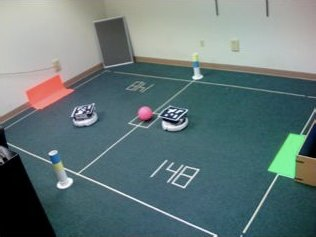
\includegraphics[width=3.04in]{figures/1_soccer1.jpg}}
\mbox{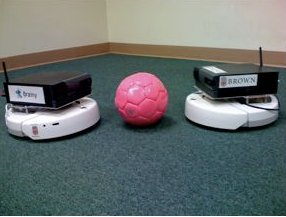
\includegraphics[width=3.00in]{figures/1_soccer2.jpg}}
}
\caption{Create platform robot soccer.}
\end{figure*}

\section{Project Deliverables}

Projects are graded assignments that consist of an implementation and a writeup.  Projects are to be implemented by student teams with individually composed written reports.  Implementations are demonstrated during scheduled class periods for grading by the course staff.  Project writeups are meant to explain student's work for the project with respect to the scientific method.  Due to the nature of robotics and programming in a nondeterministic world that is full of uncertainty, students will undoubtedly face many challenges implementing the projects. Given these challenges, experimentation and writing is essential for validating student's work.

\subsection{Project Writeups}

The purpose of the written reports is to familiarize the students with scientific writing and they should be written according to the scientific method.  The students must propose a central hypothesis, design experiments based on measurable evidence to test the hypothesis, and confirm the validity or invalidity of the hypothesis based on what was observed.  In this regard, they are not necessarily writing the document for themselves or the course staff, but rather to inform someone who is new to their work or the general topic.  Science is about general knowledge that is valid without being specific to a given time, place, or technology fads.

\section{How to use this book}

This book should be used as a hands-on guide to grounding concepts contained in the robotics textbooks (listed below) into implementable course modules.  Figure \ref{fig:1_venn} illustrates a Venn categorization of 
robotics textbooks into, ``Intro/Hobby'', ``Autonomous Robotics'', and ``Mechatronics''.  This book, as marked by the ``CS148" in Figure \ref{fig:1_venn}, is meant to combine the accessibility of an ``Intro/Hobby" (such as Martin's ``Robotic Explorations'' or Mataric's ``Robotics Primer'') with the concepts of an ``Autonomous Robotics" textbook (such as ``Principles of Robot Motion'' by Thrun et al). 
%Our aim is for anyone using this book to have both a general exposure to many robotic concepts as well as a more technical understanding of these concepts. Furthermore we provide an in depth guide on how to build a robot up through how to implement multi-robot coordination, provided general programming experience.

\begin{figure}[!h]
\centering
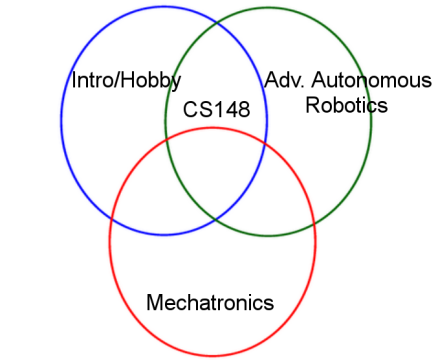
\includegraphics[width=0.5\textwidth]{figures/1_venn.png}
\caption{Types of robotic books and where CS148 falls within the spectrum.}
\label{fig:1_venn}
\end{figure}

\subsection{References}

\begin{itemize}
 
\item Matari\'c, \emph{The Robotics Primer}, MIT Press, 2007.
\item Wilson, \emph{How to Survive a Robot Uprising}, Bloomsbury USA, 2005.
\end{itemize}

\begin{wrapfigure}[10]{l}{0.15\columnwidth}
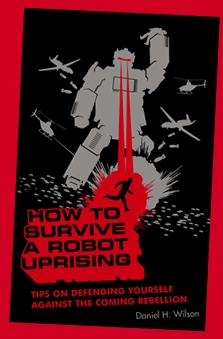
\includegraphics[height=0.25\columnwidth]{figures/1_robot_uprising.jpg}
\end{wrapfigure}

While Wilson's book has a humorous tone, it does cover many of the topics in CS148 in a substantive and accessible manner.  The other readings below are optional readings used in class.  Substantial material exists on web-accessible resources such as \href{http://wikipedia.org/}{Wikipedia} and the \href{http://www.aaai.org/aitopics/}{AI Topics Library} (specifically from the \href{http://www.aaai.org/aitopics/html/robots.html}{Robots} section).

\begin{itemize}
\item Siciliano and Khatib, \emph{Springer Handbook of Robotics}, Springer, 2008.
\item Arkin, \emph{Behavior-Based Robotics}, MIT Press, Boston, 1998.
\item Choset, Lynch, Hutchinson, Kantor, Burgard, Kavraki and Thrun, \emph{Principles of Robot Motion: Theory, Algorithms, and Implementations}, MIT Press, Boston, 2005.
\item Thrun, Burgard, and Fox: \emph{Probabilistic Robotics}, The MIT Press, 2005.
\item Martin: \emph{Robotic Explorations: A Hands-On Introduction to Engineering}, Prentice-Hall, 2001.
\item Spong, Hutchinson, and Vidyasagar, \emph{Robot Modeling and Control}, Wiley, 2005.
\item Craig: \emph{Introduction to Robotics: Mechanics and Control (3rd Edition)}, Addison-Wesley, 1989.
\item Bekey: \emph{Autonomous Robots: From Biological Inspiration to Implementation and Control}, The MIT Press, 2005.
\end{itemize}

\newpage

\rhead{Getting Started/Teleoperation}

\chapter{Getting Started/Teleoperation}
\label{sec:getting_started}

\begin{figure}[!h]
\centering
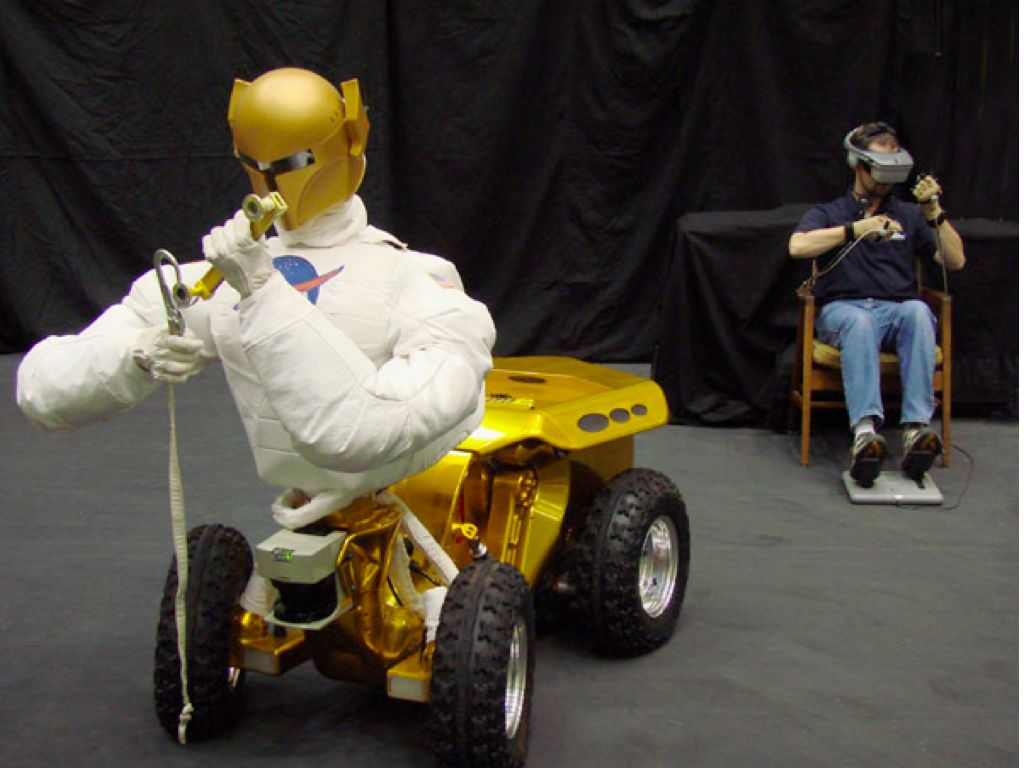
\includegraphics[width=1.0\columnwidth]{figures/2_teleop.jpg}
\end{figure}

\newpage

\begin{wrapfigure}{l}{0.55\columnwidth}
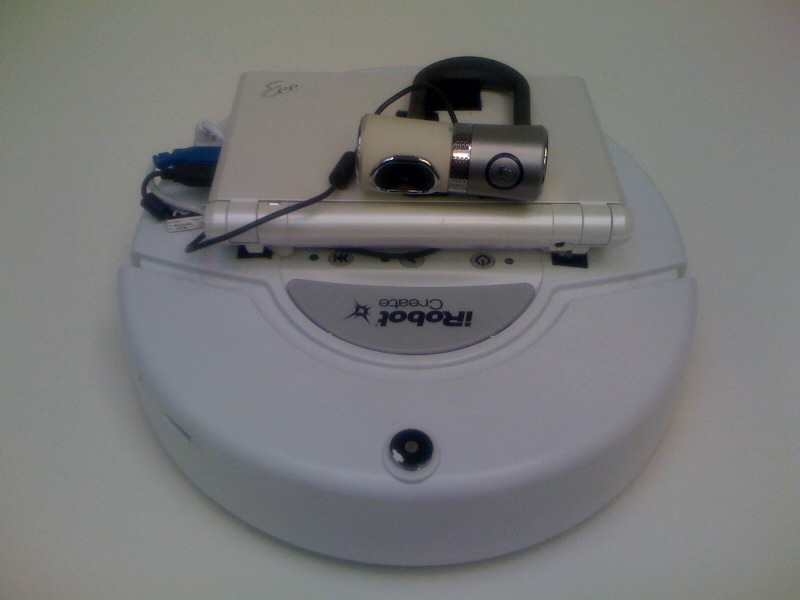
\includegraphics[width=0.5\columnwidth]{figures/2_teaser.jpg}
\end{wrapfigure}

In this chapter, we walk through the basic steps for assembling and remotely controlling a low-cost mobile robot, which we call the ``SmURV'', from ``commercial off-the-shelf'' (COTS) components.  At the completion of this chapter, you will have an assembled SmURV robot platform built with solderless commodity components. You will be able to remote control, or teleoperate, a mobile robot using one of two middleware packages we introduce in the chapter.  Instructions for hardware assembly and software installation are specified step-by-step. This chapter refers to \href{http://robotics.cs.brown.edu/projects/smurv}{The SmURV Robotics Platform}, which uses a previous version of the robot platform, and an updated version, \href{http://robotics.cs.brown.edu/projects/player\_icreate}{Setting up Player 2.1.1: Asus EeePC and iCreate Robot}. Please note, all the technology, instructions and hardware costs are as of Spring 2010.

The primary purpose of the SmURV  ({\bf Sm}all {\bf U}niversal {\bf R}obotics {\bf V}ehicle) is to be a robot platform that emphasizes the computational aspects of robotics without requiring engineering expertise or low-level hardware hacking.  That is, no soldering or low-level assembly programming is necessary to build a SmURV.  However, we do assume the reader has user-level knowledge of Unix (e.g., Ubuntu Linux, OS X) and super-user abilities to install software packages, etc.

The SmURV platform, as seen on the previous page, is based on the iRobot Create mobile base with a sub-notebook computer, such as the Asus EEE PC, and a webcam-style camera.  All of the hardware components for the SmURV can be readily purchased from online or brick-and-mortar stores, such as Target.  The computer typically runs some distribution of Linux (Ubuntu in our case) with a robot middleware package to mediate communication between a client application and the the Create/USB camera hardware.  We describe how to install robot middleware packages for Player and the Robot Operating System (ROS), although you will only need one.  Robot middleware is discussed in detail in Chapter \ref{sec:robot_middleware}.

At the end of this chapter you will be able to:
\begin{itemize}
\item Assemble a low-cost mobile robot using COTS components.
\item Install all the necessary software for running a robot client.
\item Teleoperate a mobile robot.
\end{itemize}

\section{Hardware Components}

\subsection{iRobot Create}

\begin{wrapfigure}[12]{r}{0.35\columnwidth}
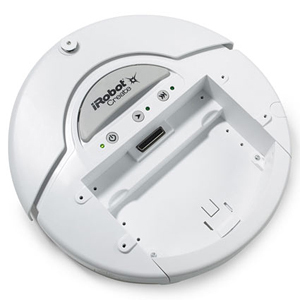
\includegraphics[width=0.3\columnwidth]{figures/2_create_base.jpg}
\end{wrapfigure}

The \href{http://store.irobot.com/shop/index.jsp?categoryId=3311368}{iRobot Create}, produced by \href{http://www.irobot.com/}{iRobot}, is used as the basic robot unit.  It is a mobile robot that is similar to the iRobot Roomba, except it does not contain a vacuum and is instead designed for robotics development.  The Create is equipped with a serial port; the \href{http://www.irobot.com/filelibrary/create/Create_Open_Interface_v6.pdf}{Open Interface Specification} (OIS) for the Create explains what commands can be sent to the Create over the serial port in order to read sensor data and send motor commands to the robot.  However, we do not 
teach students how to write programs by sending low level commands to the robot. Instead we utilize robot middleware (as explained in Chapter \ref{sec:robot_middleware}), as a hardware/software abstraction for transparency and portability.

\subsection{Accessories for the iRobot Create}
\begin{itemize}
\item \href{http://store.irobot.com/product/index.jsp?productId=2586254}{Serial Cable} that is packaged with the Create.

\item Serial to USB adapter cord.  CS148 uses FTDI US232R-10 ``evaluation cables'' which can be ordered from \href{www.digikey.com}{DigiKey} for roughly USD \$20.  Note: this cord needs to be of sufficient quality; cheaper adapters will overheat and cause problems.

\item (recommended) Rechargeable Advanced Power System (APS) Battery.

\item (optional) iRobot \href{http://store.irobot.com/product/index.jsp?productId=2731666&cp=2804606.3335976&ab=CMS_IRBT_CreateSuperCat_CreateAcc_111309&parentPage=family}{Virtual Wall} which creates an invisible barrier that the Create will not cross by emitting infrared signals that the Create detects with its IR receiver. 

\item (optional) Self Charging \href{http://store.irobot.com/product/index.jsp?productId=2598729&cp=2804606.3335976&ab=CMS_IRBT_CreateSuperCat_CreateAcc_111309&parentPage=family}{Home Base} which enables the Create to automatically charge its iRobot rechargeable battery.
\end{itemize}

\begin{figure*}
\centerline{
\mbox{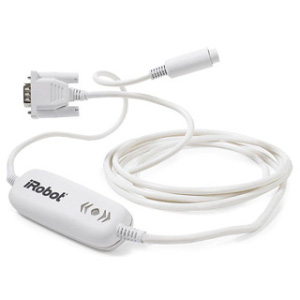
\includegraphics[width=1.50in]{figures/2_serial_cable.jpg}}
\mbox{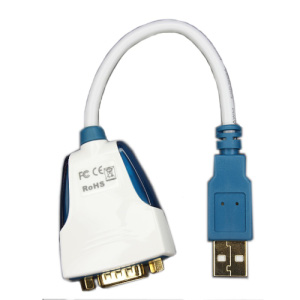
\includegraphics[width=1.50in]{figures/2_serialusb_cord.jpg}}
\mbox{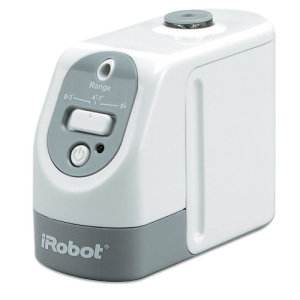
\includegraphics[width=1.50in]{figures/2_irwall.jpg}}
\mbox{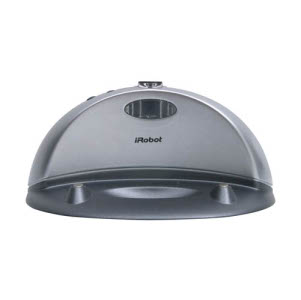
\includegraphics[width=1.50in]{figures/2_homebase.jpg}}
}
\caption{iRobot accessories include a serial cable, a serial to USB adapter, a virtual wall and a self charging home base.}
\end{figure*}

\subsection{Asus EeePC subnotebook}

\begin{wrapfigure}[8]{hr}{0.25\columnwidth}
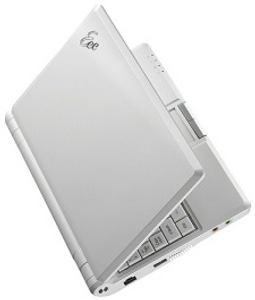
\includegraphics[width=0.2\columnwidth]{figures/2_eeepc.jpg}
\end{wrapfigure}

The \href{eeepc.asus.com/}{Asus EeePC} subnotebook is the computational brain for this robot platform.  The EeePC communicates with the Create base through a USB-Serial connection. Programs running on the EeePC will control the robot's actuators and receive sensory information. Thus the programmer does not have to worry about sending low level commands to the Create's serial port.  We recommend the \href{http://www.asus.com/index.aspx}{7'' EeePC} model since larger EeePCs will stick out over the Create base.

\subsection{USB Camera}

\begin{wrapfigure}[6]{hr}{0.25\columnwidth}
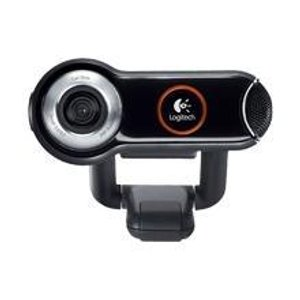
\includegraphics[width=0.2\columnwidth]{figures/2_webcam.jpg}
\end{wrapfigure}

Just having the bump, cliff and IR sensors built into the Create is not necessarily a lot of fun. Adding a camera to the robot however is! You can either go with a cheap USB Webcam or a more expensive Firewire camera if having uncompressed high quality images is a requirement. CS148 previously utilized a Unibrain Fire-I camera. However with our newest platform we recommend a USB webcam, preferably a newer, Video4Linux2 (V4L2) version.

\subsection{Assembling the Robot Platform}
\label{sec:assembling_the_robot_platform}

\begin{enumerate}
\item Connect the Create's serial cable to the USB to serial adapter. Connect this to the Create and the EeePC, as seen in Figure \ref{fig:2_cable_setup}, left image.
\item Connect the USB webcam to the EeePC.
\item Tuck the cords into the Create and set the EeePC on top. The assembled Create platform is seen in Figure \ref{fig:2_cable_setup}, right image.
\item Optionally, add Velcro tape to secure the EeePC to the top of the Create and to secure the camera to the EeePC.
\end{enumerate}

\begin{figure}[!h]
\centerline{
\mbox{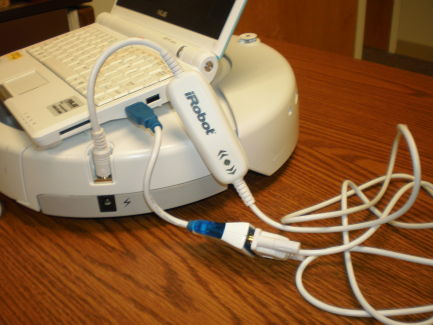
\includegraphics[width=3.00in]{figures/2_cable_setup.jpg}}
\mbox{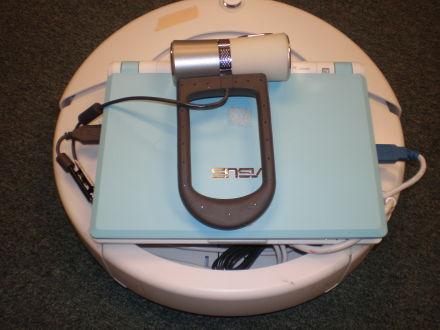
\includegraphics[width=3.00in]{figures/2_cable_store.jpg}}
}
\caption{Connected Create and EeePC; Assembled Create Robot Platform.}
\label{fig:2_cable_setup}
\end{figure}

\newpage

\subsection{Costs}

Costs are as of Spring 2010 and are specified in USD.

\begin{center}
    \begin{tabular}{ | p{3.0cm} | p{10cm} | l | l |}
    \hline
    \textbf{Part} & \textbf{Name} & \textbf{Cost} \\ \hline
    Robot (Basic) & \href{www.irobot.com}{iRobot Create Programmable Robot} & 129.99 \\ \hline
    Robot (Package) & \href{www.irobot.com}{iRobot Create Premium Development Package}; includes APS, 2 virtual walls, home base, remote and command module & 299.99 \\ \hline
    Subnotebook & \href{eeepc.asus.com}{Asus EeePC 7'' 2G Surf} & 240.00 \\ \hline
    USB Camera & \href{www.logitech.com}{Logitech Webcam Pro 9000} & 99.99 \\ \hline
    Serial to USB adapter & \href{www.digikey.com}{FTDI US232R-10 ``evaluation cables''} & 22.00 \\ \hline
    \end{tabular}
\end{center}

\section{Software Components}

\subsection{Operating System}
\label{sec:2_operating_system}

The EeePC comes with a GNU Linux OS, however we recommend installing \href{http://www.geteasypeasy.com/}{Easy Peasy (formerly Ubuntu-Eee)}, which is a custom version of Ubuntu designed especially for the EeePC.  The EeePC comes with a version of Xandros Linux which has Asus-modified libraries that are incompatible with the Player middleware system (see Section \ref{sec:player213}), thus it is recommended to simply install a more standard OS.  Easy Peasy was chosen because it is one of the more supported custom Eee Linux distributions available and it is one of the few that fits on the EeePC 2G Surf model. Note: other distributions are available and outlined on \href{http://wiki.eeeuser.com/#installing\_operating\_systems}{Installing Operating Systems}, but the rest of the instructions are assuming an Easy Peasy installation.

\subsubsection{\href{http://robotics.cs.brown.edu/projects/player_icreate/u_install.html}{Install Easy Peasy}}

\begin{enumerate}

\item You will need:
\begin{itemize}
\item Another computer to download Easy Peasy on and to run UNetbootin (Universal Netboot Installer) for creating a bootable USB flash drive. This computer must be either Windows or Ubuntu/Linux. If using Linux, you will need administrative rights to install the UNetbootin application.
\item An empty USB stick (of 1GB or more, formatted to FAT32) to do the initial Ubuntu boot and installation. 

\end{itemize}

\item From the secondary computer, go to the \href{http://www.geteasypeasy.com/}{Easy Peasy download site} and click on ``Download''.

\item Select the ``Download" link to download Easy Peasy and choose ``Save File" (Figure \ref{fig:easy_peasy}).
\begin{figure}[!h]
\centering
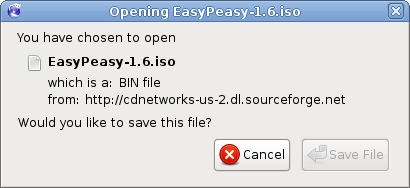
\includegraphics[width=0.5\textwidth]{figures/2_download_easypeasy2.png}
\caption{Easy Peasy download screenshot.}
\label{fig:easy_peasy}
\end{figure}


\item Download UNetbootin, a helper application used to move Easy Peasy to a USB stick. On the \href{http://unetbootin.sourceforge.net/}{UNetbootin site}, select either ``Download (for Windows)'' or ``Download (for Linux)'' depending on your operating system. Select ``Save File" (Figure \ref{fig:unetboot_download}). This step of creating a bootable drive is necessary since the EeePC does not have a CD-ROM drive.

\begin{figure}[!h]
\centering
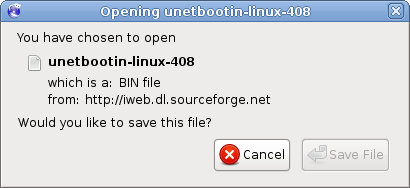
\includegraphics[width=0.5\textwidth]{figures/2_download_unetbootin.png}
\caption{UNetbootin download screenshot.}
\label{fig:unetboot_download}
\end{figure}

\item Make sure the USB stick is formatted to FAT32, otherwise the installation of Easy Peasy on the EeePC will hang and be unsuccessful. Note: formatting the stick will cause all data to be lost.

\begin{itemize}
\item To format the USB stick in Windows, insert the stick and right click on the USB icon. Press ``Format" in the menu. Select ``FAT32" in the File system drop-down list and press ``Start" (Figure \ref{fig:2_fat32}).

\begin{figure}[!h]
\centering
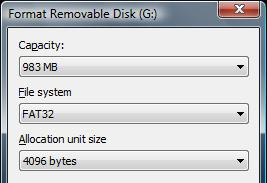
\includegraphics[width=0.35\textwidth]{figures/2_fat32.jpg}
\caption{Formatting to FAT32 in Windows.}
\label{fig:2_fat32}
\end{figure}

\item To format the USB stick in Linux, root permissions are necessary. Insert the USB stick.

\begin{enumerate}

\item Determine if the USB is already formatted to FAT32. Run: \\
\texttt{sudo fdisk -l}

\begin{figure}[!h]
\centering
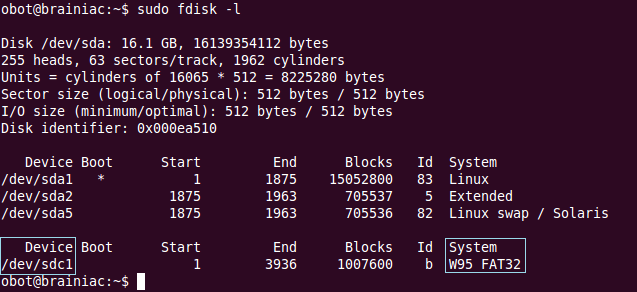
\includegraphics[width=0.66\textwidth]{figures/2_fat32_ok.png}
\caption{List USB device and current formatting.}
\label{fig:2_fat32_ok}
\end{figure}

If FAT32 is listed under ``System" (Figure \ref{fig:2_fat32_ok}), you do not need to reformat. If anything else is listed, continue.

\item Determine which device (sda, sdb, sdc, etc) Linux assigned the USB drive to. Running the above \texttt{fdisk} command prints this information under ``Device" (Figure \ref{fig:2_fat32_ok}). In our case the device assignment is to ``/dev/sdc1".\label{sec:format_usb_stick}

\item Run \href{http://linux.die.net/man/8/fdisk}{fdisk}, a partition table manipulator: \\
\texttt{sudo fdisk /dev/sdX}\\
\texttt{sdX} should be the name of the device as determined in the previous step.

\item Enter ``d" to delete all existing partitions.

\item Enter ``n" to create a new partition.\\ 
Enter ``p" for the command action.\\
Enter ``1" for the partition number.\\
Hit Enter twice to keep default settings.

\item Enter ``t" to impose the partition's system type as FAT32.\\
Enter ``b" as the partition type hex code, which is the id for type FAT32.

\item Enter ``w" to save changes and write the partition table to the USB stick.

\begin{figure}[!h]
\centering
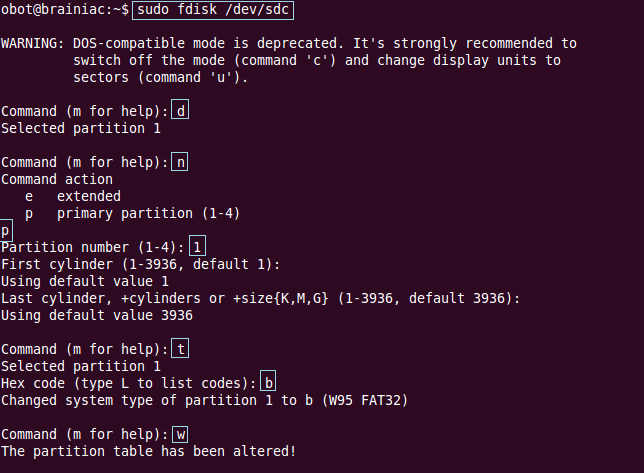
\includegraphics[width=0.66\textwidth]{figures/2_create_partition.png}
\caption{Steps (c) - (g).}
\end{figure}

\item Unmount the device: \texttt{sudo umount /dev/sdX1}

\item Format the drive to FAT32:\\
\texttt{sudo mkfs.vfat -F 32 /dev/sdX1}\\
This step is necessary in order to format the newly created partition.

\begin{figure}[!h]
\centering
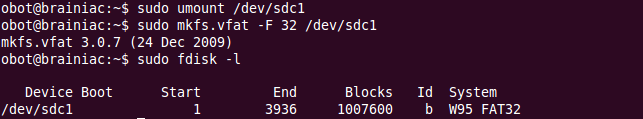
\includegraphics[width=0.66\textwidth]{figures/2_format_fat32.png}
\caption{Steps (h) - (i).}
\end{figure}

\item Unplug and insert the USB stick into the computer again.

\end{enumerate}

\end{itemize}

\item Install UNetbootin:\footnote{The following are the same instructions as under ``Installation \& Screenshots" on the \href{http://unetbootin.sourceforge.net/}{Unetbootin site}}
\begin{itemize}
\item Run the UNetbootin executable.

\begin{itemize}
\item If using Windows, click on the UNetbootin file to launch the application (Figure \ref{fig:unetboot_windows}).
\begin{figure}[!h]
\centering
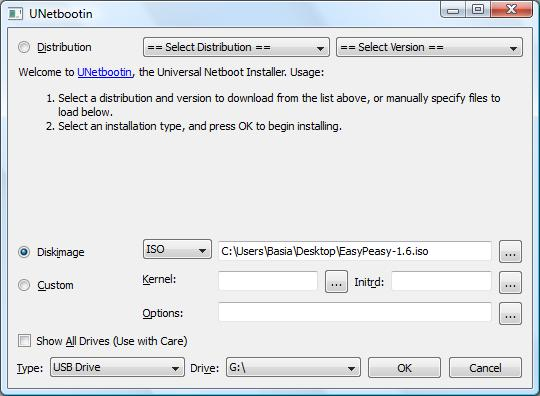
\includegraphics[width=0.85\textwidth]{figures/2_unet_windows.jpg}
\caption{UNetbootin installation prompt for Windows.}
\label{fig:unetboot_windows}
\end{figure}

\item If using Linux:\\
\begin{itemize}
\item Install Unetbootin dependencies:\\
\texttt{sudo aptitude install mtools p7zip-full}
\item Make the file executable:\\
\texttt{chmod +x unetbootin-linux-*}
\item Run the application (Figure \ref{fig:unetboot_linux}):\\
\texttt{sudo ./unetbootin-linux-*}
\end{itemize}
\begin{figure}[!h]
\centering
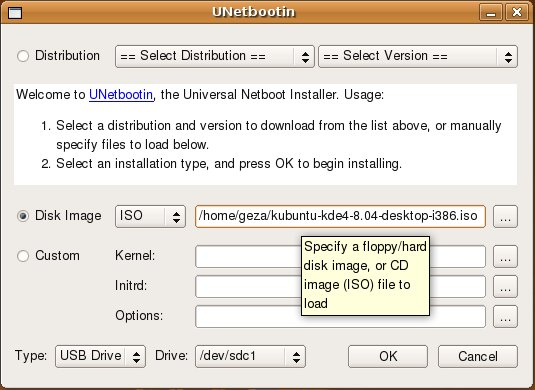
\includegraphics[width=0.85\textwidth]{figures/2_unet_linux.jpg}
\caption{UNetbootin installation prompt for Linux.}
\label{fig:unetboot_linux}
\end{figure}

\end{itemize}

\item Select Distribution/Select Version may be ignored. The Disk Image format should be ``ISO"; enter ``EasyPeasy-*.iso" (the downloaded Easy Peasy file) as the Disk Image. This specifies which file to create the bootable drive from. Finally select ``USB Drive" as the Type and specify the target Drive. Press ``OK".
\begin{itemize}
\item If using Windows, refer to Figure \ref{fig:unetboot_windows}.
\item If using Linux, refer to Figure \ref{fig:unetboot_linux}. By default, the correct USB drive should be automatically selected. To be certain, the instructions to find the name of the USB drive are outlined in step \ref{sec:format_usb_stick}.
\end{itemize}

\item After installation is complete (prompted by the screenshot in Figure \ref{fig:unetboot_install_complete}), do not reboot and instead select ``Exit" (unless you are installing Easy Peasy on the same EeePC from which you create the bootable USB drive). Unmount the disk. Easy Peasy is now installed on the USB stick.
\begin{figure}[!h]
\centering
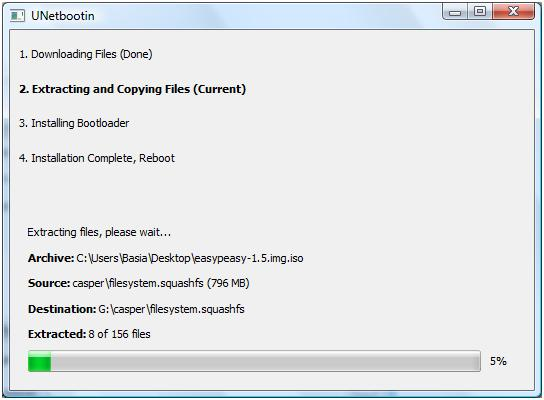
\includegraphics[width=0.85\textwidth]{figures/2_unet_windows1.jpg}
\caption{UNetbootin installation screenshot.}
\label{fig:unetboot_install}
\end{figure}

\begin{figure}[!h]
\centering
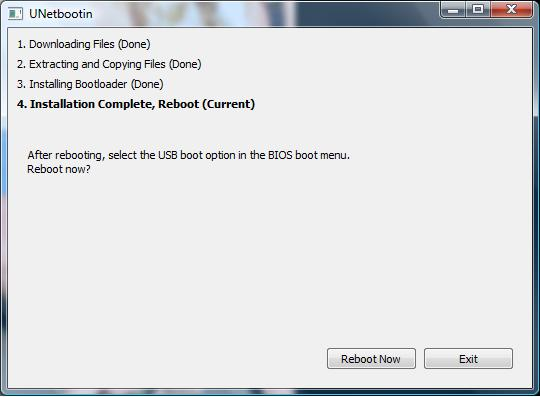
\includegraphics[width=0.85\textwidth]{figures/2_installation_complete.jpg}
\caption{UNetbootin installation complete screenshot.}
\label{fig:unetboot_install_complete}
\end{figure}

\end{itemize}

\item Insert the USB stick into the EeePC\footnote{It is suggested to use the USB port on the left side of the EeePC; some EeePC's seem unable to boot from the USB ports on the right side.}

\item (Re)start the EeePC. Press ESC a few times while the Asus boot screen is displayed.

% press F2 quickly while the EeePC is starting; this will take you to the BIOS Setup Screen. In the ``Boot" tab, select the ``Boot Device Priority" subscreen by pressing Enter. Make sure the USB drive is selected as the Boot option.

\item Select the USB drive from the list of bootable devices in the boot menu.

\item Select ``Default" from the UNetbootin menu.

\item Install Easy Peasy by selecting the ``Install EasyPeasy 1.*" icon, which should be in the Desktop folder.

\item You will be prompted for your language preference, time zone, etc. Follow all the installation instructions.

\item If your EeePC is the 2G Surf model, be aware that there is only 2GB of hard drive and the OS takes up 1.8GB when you install. Tips to prevent wasted time reinstalling:
\begin{itemize}
\item Choose ``No Localization'' on the first install screen.
\item Do a manual install, with an ext2 format and no swap drive.
\item Once installed, the 2GB internal drive will be nearly full. To free more than 300mB, uninstall Open Office, Skype and other unnecessary applications using the following command:\\
\texttt{sudo apt-get remove <package\_name>}\\
where \texttt{<package\_name>} is any package, such as \texttt{openoffice.org*}. Note, to list all installed packages: \texttt{dpkg --list}\\
\end{itemize}

\item (Optional) Enable the Regular Desktop mode instead of the Netbook Interface mode by following these \href{http://wiki.geteasypeasy.com/How_to_use_Regular_Desktop_mode_instead_of_the_Netbook_Interface_mode}{instructions}.

\item Connect the EeePC to the internet (necessary for the next step).

\item \label{sec:2_enable_repos}Enable all of the repositories in the \texttt{/etc/apt/sources.list} file. Ubuntu uses \href{http://www.debian.org/doc/manuals/apt-howto/}{APT} for package management; \texttt{/etc/apt/sources.list} contains a list of sources from which software repositories can be obtained.
\begin{itemize}
\item Backup the configuration file: \\
\texttt{sudo cp /etc/apt/sources.list /etc/apt/sources.list.backup}
\item Open the file for editing: \texttt{sudo nano /etc/apt/sources.list}
\item Enable all software repositories by uncommenting any commented-out apt repository lines (lines which begin with either ``deb" or ``deb-src"). The following are two apt lines:\\
\texttt{deb http://us.archive.ubuntu.com/ubuntu/ lucid main restricted}\\
\texttt{deb-src http://us.archive.ubuntu.com/ubuntu/ lucid main restricted}
\item Obtain the updated package lists from the newly enabled repositories:\\
\texttt{sudo apt-get update}\\
If you get the error ``Failed to fetch...", make sure the EeePC is connected to the Internet!
\item If you are outside the US and receive a ``Failed to fetch..." error, try changing all references from ``http://us.archive.ubuntu.com" to ``http://archive.ubuntu.com" in the \texttt{sources.list} file.
\end{itemize}

% \item Install software updates using the Update Manager, which can be found under ``System" $\rightarrow$ ``Administration" $\rightarrow$ ``Update Manager". DO NOT let the Update Manager remove any Ubuntu Eee specific packages (it may try).

\item Install others software packages that will be utilized: \\
\texttt{sudo apt-get install cmake subversion wget python g++}\\
If using only Player, none of these are essential for teleoperation, but cmake and subversion are at least highly recommended. If using ROS, all four of these are necessary.

\end{enumerate}


\subsection{Player 2.1.3}
\label{sec:player213}

\subsubsection{Install Player 2.1.3}
After installing Easy Peasy, the EeePC is now ready to \href{http://playerstage.sourceforge.net/doc/Player-2.1.0/player/install.html}{install Player}.

\begin{enumerate}
\item Download \texttt{player-2.1.3.tar.gz} source tarball from \href{http://sourceforge.net/projects/playerstage/files/}{Player Sourceforge Site}.

\begin{figure}[!h]
\centering
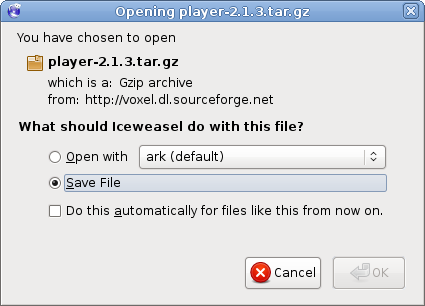
\includegraphics[width=0.5\textwidth]{figures/2_opening_player.png}
\caption{Download Player 2.1.3 screenshot.}
\label{fig:open_player}
\end{figure}

\item Uncompress and expand the downloaded file: \texttt{tar xzvf player-2.1.3.tar.gz}

\item Install additional libraries: \texttt{sudo apt-get install <library\_name>}\\
Replace \texttt{<library\_name>} with each of the following libraries: \\
libgdk-pixbuf2, libgtk2.0-dev, libjpeg62-dev.\\  
\texttt{apt-get} should have all of these libraries if every repository in \texttt{/etc/apt/sources.list} has been enabled (refer to step \ref{sec:2_enable_repos} of Section \ref{sec:2_operating_system}).
\begin{itemize}
\item If running \texttt{apt-get} gives the error: ``Couldn't find package libgdk-pixbuf2":
\begin{itemize} 
\item Add the following lines to the \texttt{/etc/apt/sources.list} file:\\
\texttt{deb http://us.archive.ubuntu.com/ubuntu/ jaunty universe}\\
\texttt{deb-src http://us.archive.ubuntu.com/ubuntu/ jaunty universe}\\
\texttt{deb http://us.archive.ubuntu.com/ubuntu/ jaunty-updates universe}\\
\texttt{deb-src http://us.archive.ubuntu.com/ubuntu/ jaunty-updates universe}\\
\item Run: \texttt{sudo apt-get update}\\
\end{itemize}

\item If you are using a fireware camera and not a USB webcam, you should also \texttt{apt-get install} the following libraries: \\ libraw1394-dev, libavc1394, libdc1394-13, libdc1394-13-dev.
\end{itemize}

\item Change to the Player source directory: \texttt{cd player-2.1.3}

\item Configure Player: \texttt{./configure}\\
Note: Player will install without throwing any errors regardless if libraries are missing. If the above mentioned libraries were not installed, Player will still install but either Player or accessing camera data may not work.

\item To enable Player to have more functionality beyond using the Create, the sensor drivers, a USB or camera, the blobfinder proxy, and playercam/playerjoy, it may be necessary to install more libraries. The libraries needed are located in the \texttt{player-2.1.3/config.log} file, which was created by configure. \texttt{config.log} is a huge file that contains all the messages created by configure, including missing packages, library dependencies and a list of what Player has and has not installed.

\item Compile Player: \texttt{make}.

\item Install Player: \texttt{sudo make install}.

\item Restart the EeePC.

\item Reopen the terminal and run Player: \texttt{player} 
\begin{itemize}
\item The output should be similar to Figure \ref{fig:player_output}.
\label{sec:player_output}

\begin{figure}[!h]
\centering
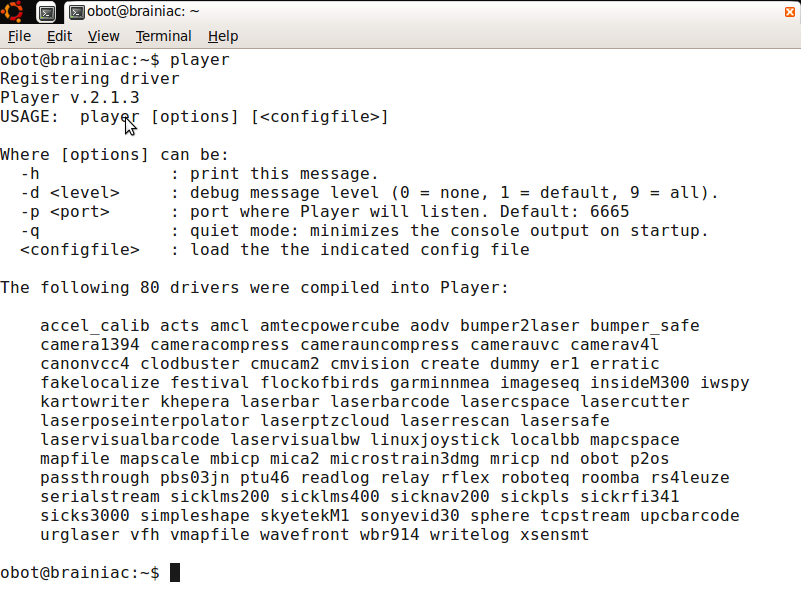
\includegraphics[width=0.85\textwidth]{figures/2_player_output.png}
\caption{Output from starting Player (Step \ref{sec:player_output} in ``Install Player 2.1.3'' instructions).}
\label{fig:player_output}
\end{figure}

\item If the following message is displayed:\\

player: error while loading shared libraries: libplayerdrivers.so.2.2: cannot open shared object file: No such file or directory\\

Run \texttt{ldconfig} to fix the error. Player sometimes does not link its libraries completely when installing.

\item If the ``Registering driver'' message outputs from Player, installation is successful and the EeePC is now ready to be hooked up to the  robot.
\end{itemize}

\end{enumerate}

\subsubsection{Run and Test Player on the Create}

To test the robot's vision and to teleoperate the Create, in this section we will be running two Player utilities that are included with the Player distribution: \href{http://playerstage.sourceforge.net/doc/Player-cvs/player/group__util__playercam.html}{playercam} and \href{http://playerstage.sourceforge.net/doc/Player-cvs/player/group__util__playerjoy.html}{playerjoy}. playercam is a GUI client that visualizes the images captured by the webcamera. playerjoy provides mobile control of the robot. The playerjoy client uses input from the keyboard to drive the robot around; only a forward and rotate speed can be manipulated on the Create.

\begin{enumerate}

\item You will need:
\begin{itemize}
\item The assembled Create Robot Platform.
\item The EeePC installed and working with Player.
\item Ideally (but not necessary to test) a wireless network and another computer with Player installed.
\end{itemize}

\item Create a configuration file, which is required by the Player server to tell Player what robot systems to load drivers for. Configuration files are text files that have a \texttt{.cfg} extension. Below is \texttt{create.cfg}, a basic configuration file for the Create with position and bumper proxies specified along with camera/blobfinder drivers. The following configuration file assumes the robot is attached to the ``/dev/ttyUSB0" port. If the robot is actually attached to a different port, reflect this change in the configuration file.

\begin{verbatim}
driver
(
        name "create"
        provides ["position2d:0" "bumper:0" "power:0" "ir:0"]
        port "/dev/ttyUSB0"
)

driver
(
        name "camerauvc"
        provides ["camera:0"]
)

driver
(
        name "cmvision"
        provides ["blobfinder:0"]
        requires ["camera:0"]
        colorfile "colors.txt"
)
\end{verbatim}

You will pass the name of this configuration file as a command line argument when starting the Player server. Please refer to Section \ref{sec:player_quickstart} for an explanation of Player configuration files and the specific format.

Note: if your EeePC has a built-in webcam, you will have to specify the external camera in the config file.
\begin{itemize}
\item Under the line:   provides [``camera:0'']   add the line:   port ``/dev/video0''.
\item Check whether your external cam is video0 or video1 by listing the contents of the \texttt{/dev} directory with the camera plugged in and unplug the camera to see which listing disappears.
\end{itemize}

\item Create a color calibration file for the blobfinder proxy. This color file is specified as \texttt{colors.txt} in the above configuration file, thus this file must reside in the same directory as \texttt{create.cfg}. Below is a generic uncalibrated color file.

\begin{verbatim}
[Colors]
(255,  0,  0) 0.000000 10 Red
(  0,255,  0) 0.000000 10 Green
(  0,  0,255) 0.000000 10 Blue

[Thresholds]
( 25:164, 80:120,150:240)
( 20:220, 50:120, 40:115)
( 15:190,145:255, 40:120)
\end{verbatim}

The following is a sample color file that has been calibrated for four different colors.

\begin{verbatim}
[Colors]
(255,  36,  0) 0.000000 10 Orange
(  0,255,  0) 0.000000 10 Green
(255,105, 180) 0.000000 10 Pink
(255, 255,0) 0.000000 10 Yellow

[Thresholds]
( 100:135, 101:115, 170:214)
( 20:220, 50:120, 40:115)
( 99:132, 123:131, 168:207)
( 124:174, 90:105, 137:148)
\end{verbatim}
Note, in a color calibration file, there must be a line space in between the Colors and the Thresholds sections. Details on what the numbers in the color file represent and how to calibrate for colors will be explained in Chapter \ref{sec:object_seeking}.

\item Put a charged battery in the Create base, turn on both the Create and the EeePC. The Led lights on the Create will blink and eventually turn off; even if the lights stop blinking the Create may still be turned on.

\item Start the Player server. Open a terminal and \texttt{cd} to the directory where your configuration file is and type: \texttt{player create.cfg}\\
\label{sec:run_player_server_output}If all is successful you should get a similar message displayed in Figure \ref{fig:player_on}.

\begin{figure}[!h]
\centering
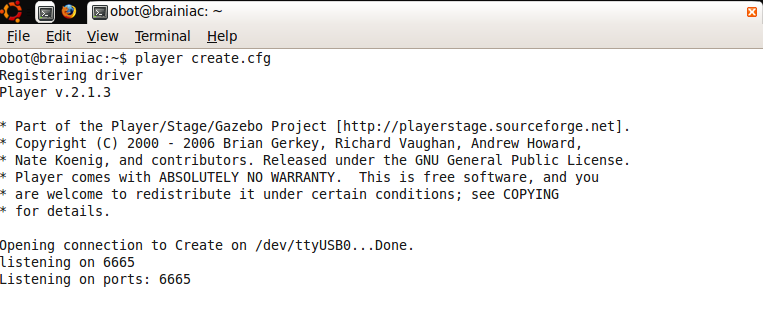
\includegraphics[width=0.85\textwidth]{figures/2_player_on.png}
\caption{Output from running the Player server with a config file (Step \ref{sec:run_player_server_output} in ``Test and Run Player" instructions).}
\label{fig:player_on}
\end{figure}

The Player server is now running on your Create Robot.

\item Run playercam. In a second terminal on the EeePC, run: \texttt{playercam}\\
Running this command will open up a window on the screen with the camera's output, as seen in Figure \ref{fig:2_playercam}. If the EeePC is on a wireless network and you want to run playercam from another computer on the network, run:\\
\texttt{playercam -h <robot IP> -p 6665} \\
\texttt{<robot IP>} is the IP address of the EeePC. The port number could be different that \texttt{6665} if you have changed from the default. 

\begin{figure}[!h]
\centering
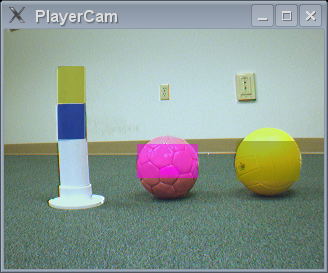
\includegraphics[width=0.5\textwidth]{figures/2_blobs.png}
\caption{Playercam output.}
\label{fig:2_playercam}
\end{figure}

If there are solid color rectangles over regions of the screen, the Player blobfinder works and is successfully detecting colors.

\item Run playerjoy to move the robot using keyboard commands. Preferably from a client computer on the network, run: \texttt{playerjoy <robot IP>:6665}. If running locally, just run: \texttt{playerjoy}. The terminal window output from running playerjoy is displayed in Figure \ref{fig:playerjoy}.
\begin{figure}[!h]
\centering
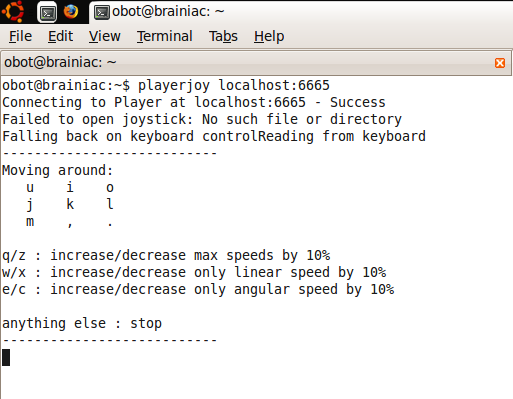
\includegraphics[width=0.6\textwidth]{figures/2_playerjoy.png}
\caption{Output from running playerjoy.}
\label{fig:playerjoy}
\end{figure}
 
Possible issues:
\begin{itemize}
\item If the robot does not move, make sure the Create base has not turned off and that the terminal with playerjoy running is selected/on top.
\item If the Create does turn off, both the player server and the client application (playerjoy or playercam) must be restarted.
\end{itemize}

\end{enumerate}


\subsection{ROS}
\label{sec:ros}

The \href{http://www.ros.org/wiki/ROS/Installation/Ubuntu/Deb}{ROS website} has installation instructions for Ubuntu that we will follow in addition to installing Brown's ROS packages. Brown University has a repository for ROS packages at \href{http://code.google.com/p/brown-ros-pkg/}{brown-ros-pkg}. Please check this site under the ``New Users" section for the latest instructions and updates on the software resources available.

\subsubsection{ROS Setup}

\begin{itemize} 

\item During the installation of Easy Peasy, make sure wget, Python, CMake and Subversion are all installed on the EeePC. If not, for any missing package needed:\\ 
\texttt{sudo apt-get install cmake subversion wget python}

\item Setup sources.list:\\
\texttt{sudo sh -c 'echo "deb http://code.ros.org/packages/ros/ubuntu karmic main" > /etc/apt/sources.list.d/ros-latest.list'}

\item Set up your keys:\\
\texttt{wget http://code.ros.org/packages/ros.key -O - | sudo apt-key add -}

\item Run: \texttt{sudo apt-get update}

\item Install: \texttt{sudo apt-get install ros-boxturtle-base}\\
Alternatively, for the latest release, run: \\
\texttt{sudo apt-get install ros-latest-base}

% \item Uninstall ros-specific packages???

\item Brown has a ROS install script available which retrieves versions of the ROS source, tested to be compatible with brown's packages, and automatically retrieves the latest brown packages. To retrieve the install script, on the EeePC run:\\
\texttt{wget http://brown-ros-pkg.googlecode.com/svn/tags/getros/getros.py}

\item Run the script to install: \texttt{python getros.py}

\item To setup the correct environment variables, from the ROS root directory run:\\ \texttt{source rosenv}\\
You must do this everytime you open up a new terminal.

\item Build the basic ROS packages with: \texttt{rosmake roslite} \\
Each brown-ros-pkg package can be build with appropriate calls to rosmake, such as: \texttt{rosmake cv\_capture}. Note, the \texttt{rosmake} command can be run from any directory within the ROS directory structure.

% sudo apt-get install python-yaml libapr1-dev libbz2-dev python-dev libaprutil1-dev python-numpy graphviz

%YAML
% If you receive a compile error: ``ImportError: No module named yaml", you need to install YAML.
% download from: http://pyyaml.org/wiki/PyYAML
% tar zxvf PyYAML-*.tar.gz
% cd PyYAML-*
% python setup.py instal

% LOG4CXX
% cd ~/ros/ros-deps 
% wget http://pr.willowgarage.com/downloads/apache-log4cxx-0.10.0-wg_patched.tar.gz
% tar xzf apache-log4cxx-0.10.0-wg_patched.tar.gz
% cd apache-log4cxx-0.10.0
% ./configure --prefix=/opt/ros
% make
% sudo make install 

% BOOST
% cd ~/ros/ros-deps
% wget --tries=10 http://pr.willowgarage.com/downloads/boost_1_37_0.tar.gz
% tar xzf boost_1_37_0.tar.gz
% cd boost_1_37_0
% ./configure --prefix=/opt/ros
% make
% sudo make install 

\end{itemize}

\subsubsection{Run and Test the Brown ROS Create Driver}

\begin{itemize}

\item The \href{http://code.google.com/p/brown-ros-pkg/wiki/irobot\_create\_2\_1}{Brown ROS Create Driver} is located in the ``ros-1.0.0/pkg/irobot\_create\_2\_1" directory. 


% PYTHON-SERIAL
% tar zxvf pyserial-*.tar.gz
% cd pyserial-*
% python setup.py install
 

\item \href{http://pyserial.sourceforge.net/}{python-serial} is the only external dependency of the driver and must be installed.
\begin{itemize}
\item Go to \href{http://sourceforge.net/projects/pyserial/files/}{pyserial} to download.
\item Unpack the archive and install the package: \\
\texttt{tar zxvf pyserial-*.tar.gz}\\
\texttt{cd pyserial-*}\\
\texttt{python setup.py install}
\end{itemize}

\item Build: \texttt{rosmake irobot\_create\_2\_1}

\item In its own terminal run: \texttt{roscore}\\
This command launches the ROS Master, which must be running for other ROS nodes to locate each other and communicate.

\item The ROS Create node assumes the robot is attached to ``/dev/ttyUSB0". If it is not, run: \texttt{rosparam set /brown/irobot\_create\_2\_1/port PORT}\\
PORT should be the port to which the robot is actually attached to.

\item Run the create driver: \texttt{rosrun irobot\_create\_2\_1 driver.py}\\
This command runs the Create driver from the Brown ROS package. The purpose of this node is to provide other nodes with basic sensor information (e.g. whether or not a bumper has been pressed), as well as to provide basic movement control to other nodes for the Create.

\item Teleoperate the Create using the ``teleop\_twist\_keyboard" package.
\begin{itemize}
\item Compile: \texttt{rosmake teleop\_twist\_keyboard}
\item Run: \texttt{rosrun teleop\_twist\_keyboard teleop\_twist\_keyboard.py}
This teleoperates the robot using keyboard commands (Figure \ref{fig:2_teleop_twist}).
\end{itemize}

\begin{figure}[!h]
\centering
\includegraphics[width=0.8\textwidth]{figures/2_teleop_twist.png}
\caption{Teleoperating the Create using ROS}
\label{fig:2_teleop_twist}
\end{figure}


\end{itemize}

\newpage

\rhead{Robot Middleware}

\chapter{Robot Middleware and Controller Development}
\label{sec:robot_middleware}

\begin{figure}[!h]
\centering
\includegraphics[width=0.5\columnwidth]{figures/3_abstraction.jpg}
\label{fig:3_abstraction}
\caption{Middleware layers.}
\end{figure}
\newpage

\begin{wrapfigure}{r}{0.55\columnwidth}
\includegraphics[width=0.53\columnwidth]{figures/3_app_store.jpg}
\end{wrapfigure}

Given a robot embodiment and a program that controls the robot, middleware serves as an abstraction between the hardware and the robot client that allows for writing robot controllers not dependent on any specific platform, as seen in Figure \ref{fig:3_abstraction}\footnote{Source: Golftheman, http://en.wikipedia.org/wiki/File:Operating\_system\_placement.svg}. The need for robot middleware arises out of the question of how to program our robots to perform desired tasks. The straightforward approach is to write and compile a program that directly sends low level commands to the robot base in order to perform the robot's ``cognitive'' functions. This one-off solution may be sufficient for programming the robot to perform one specific task on top of one specific robot platform.  However, the following challenges arise from applying this approach to robotic application development:

\begin{itemize}
\item Portability to other robot platforms or new devices.
\item Scalability to growth in functionality.
\item Reusability for other projects.
\item Interoperability between functions and languages.
\end{itemize}

To enhance the application development for robots, middleware services exist to provide an abstraction layer between computation and embodiment, similar to the hardware abstraction layer in operating systems. Middleware allows any robot controller to run on any robot platform, thus the controller software is not specific to the hardware. Between the hardware at the lowest layer and a client program at the highest layer is the middleware, which provides an interface to the robot's devices and marshals the high level commands of the client program to the low level commands understandable by the robot hardware. Middleware aims to overcome the above listed challenges by simplifying the development process, enhancing software integration and reuse, supporting interoperability, providing efficient utilization of robot components and resources, and providing interfaces that hide the low-level hardware complexity.

Although the Create platforms we are using in CS148 are relatively simple since we only need access to a handful of sensors and actuators, many robotic applications today are complex assemblages, consisting of many heterogeneous hardware components build by different manufacturers, and multiple software modules written in different languages. Given such a platform, the need for middleware is essential, allowing for modular design while coordinating the communication among the components efficiently and providing interoperability, portability and robustness.

There are several existing middleware packages for robotics, such as \href{http://code.google.com/p/lcm/}{LCM}, \href{http://www.orocos.org/}{Orocos}, \href{http://eris.liralab.it/yarp/}{YARP}, \href{http://carmen.sourceforge.net/}{CARMEN}, \href{http://msdn.microsoft.com/en-us/robotics/default.aspx}{Microsoft Robotics Studio} and JAUS. This course focuses on two: Player and the Robot Operating System, although there is mention of other middleware systems as well.

At the end of this chapter you will be able to:
\begin{itemize}
\item Understand the Player and/or ROS robot middleware system as an abstraction between the robot hardware and software.
\item Understand the basic concepts of a handful of other middleware systems.
\item Know how to send commands to and receive sensory information from the robot using either Player or ROS.
\item Write a basic robot client application to control the robot.
\end{itemize}

\section{Player/Stage/Gazebo}

\href{http://playerstage.sourceforge.net}{PSG} is a robot interface and simulation software suite that expose drivers through a simple interface for robotic applications. The core of PSG is the \href{http://playerstage.sourceforge.net/wiki/Player}{Player robot interface}, which is a framework for robot control consisting of devices, robot servers and robot clients.

\begin{figure}[!h]
\label{fig:PlayerMiddleware}
\centering
\includegraphics[width=0.8\columnwidth]{figures/3_player_abstraction.png}
\caption{Player middleware abstraction.}
\end{figure}

Running on your robot, Player provides a clean and simple interface to the robot's sensors and actuators over a TCP/IP (or UDP/IP) network. Client programs talk to Player over a TCP socket, read data from sensors, write commands to actuators, and configure devices on the fly. Figure \ref{fig:PlayerMiddleware}\footnote{Source: http://www.ki.inf.tu-dresden.de/~wiki/Robotics/Creatures/PlayerTutorial.pdf} illustrates the Player middleware abstraction between hardware and client applications.

One of the major advantages of Player as a robot server is its independence from a particular client-development language.  The interaction between Player and a client program is done completely over a TCP/IP (or UDP/IP) network connection. The communication between the Player client and Player server are illustrated in Figure \ref{fig:ClientServer}\footnote{Source: http://www.ki.inf.tu-dresden.de/~wiki/Robotics/Creatures/PlayerTutorial.pdf}.  Thus, any language with libraries that supports Player functionalities can be used to develop robot clients.  The best-supported client languages are C and C++ (supported through libplayerc and libplayerc++). Client programs can run on any machine that has a network connection to your robot and can be written in any language that supports TCP sockets. Additionally Player is designed to be platform independent; it supports a variety of robot hardware and Player's modular architecture makes it easy to add support for new hardware.

\begin{figure}[!h]
\centering
\includegraphics[height=0.45\columnwidth]{figures/3_communication.png}
\caption{\label{fig:ClientServer}Client/server communication.}
\end{figure}

Player is complemented by two simulation systems, \href{http://playerstage.sourceforge.net/wiki/Stage}{Stage} and \href{http://playerstage.sourceforge.net/wiki/Gazebo}{Gazebo}.  Stage simulates a population of mobile robots, sensors and objects in a two-dimensional bitmapped environment. Stage is designed to support multi-agent autonomous systems, so it provides fairly simple, computationally cheap models of lots of devices rather than attempting to emulate any device with great fidelity.  Gazebo is a physically simulated multi-robot simulator. Like Stage, it is capable of simulating a population of robots, sensors and objects, but does so in a physically dynamic three-dimensional world using the \href{http://www.ode.org/}{Open Dynamics Engine}. It generates both realistic sensor feedback and physically plausible interactions between objects with higher computational overhead.  These simulation systems are often an excellent means to prototype robot controllers.  However, these simulators do not have the same uncertainty and nondeterminism as faced in the real world.  We strongly recommend to students to thoroughly testing their controllers on a real robot before demoing or submitting assignments.

\subsection{Client/Server Architecture}

\begin{wrapfigure}[21]{r}{0.4\columnwidth}
\centering
\includegraphics[height=0.5\columnwidth]{figures/3_player_model.jpg}
\caption{\label{fig:player_model}The Player model's layers of abstraction.}
\end{wrapfigure}

 
Player is a device server that provides an interface to robots, sensors and actuators. The components of the Player model is illustrated in Figure \ref{fig:player_model}\footnote{Source: http://psurobotics.org/wiki/index.php?title=Player/Stage\_Drivers}.

Devices (e.g., a laser, a camera, or a complete robot) are the actual hardware in the real world or simulated hardware that exists in a virtual environment maintained by Stage or Gazebo. Hardware resides at the lowest level in this model.

A robot server (e.g., Player) is the information interface between the robot and any program that requests information from or sends commands to the robot.  Regardless of whether a device is real or simulated, the robot server provides the same interface to the robot for client programs.  Thus, controllers developed on a simulated device will immediately run the equivalent real robot device.  (Note: A robot's {\bf behavior} is a function of both its controller and environment.  A robot controller working in one environment does not necessarily imply the same controller will yield the same behavior in new or similar environments, given PSG support for the device.)

A robot client, at the highest level in this model, is a user-developed program that accesses robot functions through the robot server.  The robot client will first establish a connection to the robot's server and then command the robot by reading data from the server and sending appropriate control command back.  The job of the developer is to write control programs that produce commands that yield desired behavior from information received from the robot server\footnote{Referring to the lecture on autonomous control, the description of the robot client should remind you of feedback control (i.e., commands [$u_t$] that produce desired state [$x_d$] given observations [$y_d$]).}  

Proxies are used by the client to retrieve information from a sensor or control an actuator; they expose interfaces to both hardware devices and existing implemented algorithms. 

Drivers reside on top of the robot and provide access to specific functions of the robot. 

Player uses a TCP socket-based client/server model, illustrated in Figure \ref{fig:ClientServer}. The client is a given robot application which interacts with the server running on the robot. The server exposes devices as proxies and publishes data continuously. The client first establishes a network connection with the robot server and subscribes to robot proxies. The client then runs in a continual loop, receiving data from and sending actuator commands to the server. Because Player follows a publish/subscribe messaging paradigm to control the robot over a network, there is no dependency on which programming language robot applications are written in\footnote{Given that the programming language has a Player client library to provide the appropriate messages, such as libplayerc for the C language.} and clients can execute from any computer on the network.
 
\subsection{Proxies}
 
The server continually publishes proxy information and the client sets variables to subscribed proxies to control the robot. The information being sent over the network between the client and server is only with respect to the proxies the client explicitly initialized. 

The proxies that are of interest to applications written in CS148:
\begin{itemize}
\item position2d: controls mobile robot bases in 2D. Client sends motor commands for velocity control by setting a forward and rotate speed to the robot; allows access to the odometric information.
\item bumper: returns data from the bumper device. This proxy accepts no commands.
\item ir: provides access to an array of infrared (IR) range sensors. The ir proxy controls two sets of ir devices on the Create. The first is a small infrared on the tip of the Create that senses virtual walls; the second set are four ir sensors on the bottom of the Create for detecting cliffs on the ground.
\item camerauvc: allows access to a USB camera and retrieves images from a camera device.
\item blobfinder: provides access to devices that detect blobs in images used for color recognition. 
\end{itemize} 

The full list of device proxies can be found \href{http://playerstage.sourceforge.net/doc/Player-cvs/player/group\_\_playerc\_\_proxies.html}{here}.

\subsection{Player Quick Start with Create}
\label{sec:player_quickstart}

The following are instructions on how to use Player as a middleware
abstraction to send commands to a robot. This is an example of client
application in C++ that controls an iRobot Create to continually
rotate in place and read bumper information from the robot.

\begin{enumerate}

\item \label{sec:3_create_client}Create a \texttt{client.cpp} program using the code below.

\begin{verbatim}
#include <stdio.h>
#include <libplayerc++/playerc++.h>
#include <signal.h>

//Use the player namespace, for cleanliness
using namespace PlayerCc;

//declare Ctrl-C-related variables
bool endnow = false;
//function to receive signals
void stopper(int x)
{
  endnow = true;
}

int main(int argc, char** argv)
{
  //Player setup
  PlayerClient *client = new PlayerClient(argv[1],6665);
  client->SetDataMode(PLAYER_DATAMODE_PULL);
  client->SetReplaceRule(true,-1,-1);

  // Create a position2d proxy (device id "position2d:0") and susbscribe
  // in read/write mode
  Position2dProxy *posProxy = new Position2dProxy(client,0);
  //set the robot to be stationary
  posProxy->SetSpeed(0,0);

  // Create a bumper proxy and subscribe
  BumperProxy *bumperProxy = new BumperProxy(client, 0);

  //tell the function 'stopper' to receive all SIGINT signals.
  signal(SIGINT,stopper);
  while(!endnow)
  {
    // read from the proxies
    client->Read();

    double forward = 0.0;
    double rotate = 0.3;
	
    printf("Forward is %g, rotate is %g.\n",forward,rotate);
    printf("Left: %d     Right: %d\n",
    bumperProxy->IsBumped(0),bumperProxy->IsBumped(1));
    // send commands to control the motors
    posProxy->SetSpeed(forward,rotate);
  }
  posProxy->SetSpeed(0,0);
		
  //cleanup
  delete posProxy;
  delete bumperProxy;		
  delete client;
		
  return 0;
}
\end{verbatim}

This program uses \texttt{libplayerc++}, which is a C++ client library for the Player server. Because libplayerc++ is used in this example, the position2d and bumper device proxies are not directly accessed. Instead the Position2dProxy and BumperProxy classes are used which control the position2d and bumper devices, respectively. Please see the \href{http://playerstage.sourceforge.net/doc/Player-cvs/player/classPlayerCc\_1\_1Position2dProxy.html}{Position2dProxy Class Reference} and the\href{http://playerstage.sourceforge.net/doc/Player-cvs/player/classPlayerCc\_1\_1BumperProxy.html}{BumperProxy Class Reference} for the public member functions of each class.

 This client first creates a PlayerClient proxy and establishes a connection to the server on the IP specified in the command-line argument (which can just be ``localhost'') listening on port 6665. PositionProxy and BumperProxy objects are created, using the client proxy object to establish access to the position2d and bumper devices. The program enters a loop (that may be exited using Ctrl-c) that spins the robot in place by sending commands to control the actuators by setting the velocity via the position2d proxy. Furthermore the client accesses the sensory information from the bumper proxy to determine if the bumper is currently pressed.

\item \label{sec:3_config_file}As described in \ref{sec:player213}, a Player configuration file must reside in a directory on the robot where you will start the Player server. Configuration files are used to inform the Player server which drivers need to be instantiated. The config file consists of driver sections, declared by the keyword \texttt{driver()}, which configure drivers. A driver section is composed of option-value pairs that are whitespace separated. Both the \texttt{name} and \texttt{provides} options are required in a driver section. The \texttt{provides} keyword specifics the device address(es) through which the driver can be accessed. The \texttt{requires} keyword specifies the device address(es) to which the driver will subscribe.

Below is a sample \texttt{create.cfg} used for this exercise:

\begin{verbatim}
driver
(
        name "create"
        provides ["position2d:0" "bumper:0" "power:0" "ir:0"]
        port "/dev/ttyUSB0"
)

driver
(
        name "camerauvc"
        provides ["camera:0"]
)

driver
(
        name "cmvision"
        provides ["blobfinder:0"]
        requires ["camera:0"]
        colorfile "colors.txt"
)
\end{verbatim}

\noindent Please refer to the \href{http://playerstage.sourceforge.net/doc/Player-1.6.5/player-html/configfile.php}{configuration files link} and the tutorial \href{http://playerstage.sourceforge.net/doc/Player-2.1.0/player/group\_\_tutorial\_\_config.html}{writing configuration files} to learn more about config files.

\item pkg-config, a tool that searches for installed libraries when compiling, must know where libplayerc++ is installed. By default the pkg-config files for Player are installed in /usr/local/lib/pkgconfig and this directory should be in the search path for pkg-config. \\
Run: \texttt{pkg-config --libs playercore}\\
If the output is similar to ``-lplayercore -lltdl -lpthread -lplayererror", you should be fine. Otherwise you will have to set the PKG\_CONFIG\_PATH environment variable to include the /usr/local/lib/pkgconfig path\footnote{Source: http://playerstage.sourceforge.net/doc/Player-2.1.0/player/install.html}:\\
\texttt{export PKG\_CONFIG\_PATH=/usr/local/lib/pkgconfig:\$PKG\_CONFIG\_PATH}

\item Compile the client application:\\
\texttt{g++ -o client `pkg-config --cflags playerc++` client.cpp `pkg-config --libs playerc++`}\\
(Best to copy and paste this line; note the above single quotes are a different ASCII character then the typical single quote and you will get a compile error if this is not correct).

\item Turn on the Create base and the EeePC.

\item Start the Player server on the robot: \texttt{player create.cfg}

\item Run the client application.
\begin{itemize}
\item If locally executing the client: \texttt{./client localhost}.
\item If the robot is on a wireless network, run the following from another computer on the network: \texttt{./client <robot IP>} where \texttt{<robot IP>} is the IP address of the robot.
\end{itemize}

\end{enumerate}

\noindent Please refer to the Player website for a simple \href{http://playerstage.sourceforge.net/doc/Player-2.1.0/player/group\_\_libplayerc\_\_example.html}{Player C example}, and also for another \href{http://playerstage.sourceforge.net/doc/Player-2.1.0/player/group\_\_cplusplus\_\_example.html}{Player C++ example}.

\section{ROS}

ROS is a robotics software framework that provides an interface to the
robot's sensors and actuators over an IP network. ROS enables a
peer-to-peer network of distributed processes that process data
together and use the ROS communication infrastructure.  According to
the system's developers:
 
\begin{quote}
\href{http://www.ros.org/wiki/ROS/StartGuide}{Robot Operating System (ROS)}, a \href{http://www.willowgarage.com/}{Willow Garage} software platform, is an open-source, meta-operating system for your robot. It provides the services you would expect from an operating system, including hardware abstraction, low-level device control, implementation of commonly-used functionality, message-passing between processes, and package management. It also provides tools and libraries for obtaining, building, writing, and running code across multiple computers. 
\end{quote}

\subsection{Peer-to-Peer Messaging Model}

%GRAPHIC OF CONTROLLED SERVER
\begin{figure}[!ht]
\centering
\includegraphics[width=39pc]{figures/3_rosmaster.pdf}
\caption{\label{fig:master} A conceptual view of a higher-level node calling a lower-level node. The master node is responsible for matching nodes to enable communication between them (source unknown).}
\end{figure}

\begin{figure}[!ht]
\centering
\includegraphics{figures/3_master-node-example.png}
\caption{\label{fig:master_node_example} A diagram of controlling a Hokuyo laser range-finder. Details can be found at the \href{http://www.ros.org/wiki/ROS/Technical\%20Overview}{ROS website}.}
\end{figure}

ROS uses a peer-to-peer architecture over a TCP network, allowing for
various styles of communication. The basic building block in ROS is
a \emph{node}.  Each node is a modular process with some specialized
purpose. A particular node, for example, might implement a robot's
basic motor control, or publish information from a camera.
Furthermore, these simple nodes may be combined in various ways to
form more complex nodes governing more sophisticated behaviors.  For
instance, an obstacle-avoidance node may combine information from a
robot's sensors, actuators and higher-level control architecture to
compute a maneuver.  A primary motivation of ROS is to promote code
reuse, and the modularity and platform-independence of nodes helps
serve this purpose.

\begin{wrapfigure}{r}{0.35\columnwidth}
\centering
\includegraphics[width=0.3\columnwidth]{figures/3_ros_messaging.png}
\caption{\label{fig:ros_messaging}ROS messaging.}
\end{wrapfigure}

Nodes communicate with each other by publishing messages
to \emph{topics}, which are the basic message structure for
broadcasting data. Nodes publish messages to a topic as well as subscribe
to a topic to receive messages, as seen in
Figure \ref{fig:ros_messaging}\footnote{Source: http://www.ros.org/wiki/ROS/Concepts}. 
Thus topics are intended for
unidirectional, streaming communication. In general, nodes are not
aware of who they are communicating with. Instead, nodes that are
interested in data subscribe to the relevant topic; nodes that
generate data publish to the relevant topic. Figure \ref{fig:master_node_example}\footnote{Source: http://www.ros.org/wiki/ROS/Technical\%20Overview} 
provides an illustration of communication between nodes; the ``hokuyo" node 
publishes messages on the ``scan" topic and the ``viewer" node subscribes to the
``scan" topic. The two nodes are decoupled and need not know of each other.
 
Nodes that need to perform remote procedure calls, i.e. receive a
response to a request, should use \emph{services} instead. Unlike the
publish/subscribe communication paradigm that topics provide, services
allow for Remote Procedure Call (RPC) request/reply interactions which
are often required in a distributed system. Request/reply is done via
a Service, which is defined by a pair of Messages: one for the request
and one for the reply.

A complex program could potentially consist of tens or hundreds of
nodes, and these nodes need some efficient way to communicate with
each other. Thus, every program in ROS is run with a special node
called the \emph{master node}. Conceptually, this node is a
matchmaker: it is responsible for listening to node offers and
requests, and then introducing relevant nodes to each other so that
they can communicate. The master nodes provides naming and
registration services to the rest of
the \href{http://www.ros.org/wiki/Nodes}{nodes} in the ROS system. They
track publishers and subscribers
to \href{http://www.ros.org/wiki/Topics}{topics} as well
as \href{http://www.ros.org/wiki/Services}{services}. Thus the role of
the master nodes is to enable individual ROS nodes to locate one
another. Once these nodes have located each other they communicate
with each other peer-to-peer.

ROS client libraries for various programming languages,
(eg \verb/roscpp, rospy, rosjava/) exist that facilitate the
developer to program ROS nodes, publish and subscribe to topics, and
write and call services.
 
In addition to being a robot middleware system, ROS provides package
management along with an integrated build system. It also provides
tools and libraries for obtaining, building, writing, and running code
across multiple computers. Finally ROS allows for integration of
external packages, repositories and third-party software such as
OpenCV, OpenRAVE and even Player.

\subsection{ROS Quick Start with Create}
\label{sec:ros_quickstart}

The \href{http://code.google.com/p/brown-ros-pkg/}{Brown ROS package} is a set of nodes that provides basic sensing and movement functionality for the iRobot Create. This section demonstrates creating an \texttt{irobot\_create\_controller} node and writing a controller that provides a simple method to determine whether the robot's left or right bumper is pressed, as well as to set the robot's speed and rotation. This controller will rotate the Create in place until Ctrl-c is pressed.

\begin{itemize}

\item From the ROS root directory on the EeePC: \texttt{cd ros-1.0.0/pkg}\\
(Don't forget to \texttt{source rosenv} from the ROS root directory).

\item Create a ROS package for our controller:\\
\texttt{roscreate-pkg irobot\_create\_controller roscpp std\_msgs irobot\_create\_2\_1}\\
The \texttt{roscreate-pkg} command-line tool automatically creates a new ROS package called \texttt{irobot\_create\_controller} with dependencies on three other packages (\texttt{roscpp}, \texttt{std\_msgs} and \texttt{irobot\_create\_2\_1}). It generates a number of files for building the new package.

\item Create a \texttt{client.cpp} file in \texttt{irobot\_create\_controller/src} and add the following code to \texttt{client.cpp}:

\begin{verbatim}
#include <ros/ros.h>
#include <irobot_create_2_1/SensorPacket.h>
#include <geometry_msgs/Twist.h>
#include <signal.h>

ros::Publisher create_pub;
ros::Subscriber create_sub;

// Declare Ctrl-C related variables
bool endnow = false;
void stopper(int x)
{
  endnow = true;
}

// Master node calls this function everytime a new message arrives
void createListen(const irobot_create_2_1::SensorPacketConstPtr& msg)
{
  printf("Left: %d, Right: %d\n", msg->bumpLeft, msg->bumpRight);  
}

int main(int argc, char** argv) {

  // Initialize ROS
  ros::init(argc, argv, "controller");
  // Create a handle to this process node
  ros::NodeHandle n;
  // Publish messages of type geometry_msgs/Twist on topic "cmd_vel"
  create_pub = n.advertise<geometry_msgs::Twist>("cmd_vel", 1);
  // Subscribe to the "sensorPacket" topic.
  create_sub = n.subscribe("sensorPacket", 0, createListen);

  // Tell the function 'stopper' to receive all SIGINT signals	
  signal(SIGINT,stopper);

  while(!endnow)
    {
      double forward = 0.0;
      double rotate = 0.3;

      // Create and publish a Twist message
      geometry_msgs::Twist twist;
      twist.linear.x = forward; twist.linear.y = 0; twist.linear.z = 0;
      twist.angular.x = 0; twist.angular.y = 0; twist.angular.z = rotate;
      create_pub.publish(twist);

      ros::spinOnce();
    }

  // Stop the robot's movement
  geometry_msgs::Twist twist;
  twist.linear.x = 0; twist.linear.y = 0; twist.linear.z = 0;
  twist.angular.x = 0; twist.angular.y = 0; twist.angular.z = 0;
  create_pub.publish(twist);

  printf("Done.\n");
	
  return(0);
}
\end{verbatim}

The Create driver publishes a single message type, \texttt{SensorPacket.msg}, which exports all of the robot's sensory information. The message file exists in:\\ ros-1.0.0/pkg/irobot\_create\_2\_1/msg/SensorPacket.msg\\ 
For online documentation, visit the Brown ROS Create Driver \href{http://code.google.com/p/brown-ros-pkg/wiki/irobot\_create\_2\_1}{site}.

Additionally, use this \href{http://www.ros.org/wiki/ROS/Tutorials/WritingPublisherSubscriber(c\%2B\%2B)}{ROS tutorial} as a helpful resource for writing simple Publish and Subscriber nodes in C++.

\item Edit \texttt{irobot\_create\_controller/CMakeLists.txt} and add the following line to the end of the file:\\
\texttt{rosbuild add executable(client src/client.cpp)}\\
This causes an executable named \texttt{client} to be created whenever you run the command \texttt{rosmake irobot\_create\_controller}. For more information on CMake, refer to Section \ref{sec:3_cmake}, however most of the work in creating CMakeLists is done automatically by ROS.

\item Compile: \texttt{rosmake irobot\_create\_controller}

\item Turn on the Create base.

\item Run the ROS master: \texttt{roscore}

\item Run the Create driver: \texttt{rosrun irobot\_create\_2\_1 driver.py}

\item Run the controller client: \texttt{rosrun irobot\_create\_controller client}

\end{itemize}

\section{Other Middleware Packages}

There are many suitable robot middleware packages beyond Player and ROS, some of which are described in brief below.  For an excellent comparison of robot middleware, we refer the reader to the survey and analysis conducted by Huang et. al.\footnote{Huang, Olson and Moore, \textit{Lightweight Communications and Marshalling for Low Latency Interprocess Communication}, Technical Report MIT-CSAIL-TR-2009-041, 2009.}

\subsection{LCM}

\href{http://code.google.com/p/lcm/}{Lightweight Communications and Marshalling (LCM)} is ``a library for message passing and data marshalling targeted at real-time systems where high-bandwidth and low latency are critical. It provides a publish/subscribe message passing model and an XDR-style message specification language with bindings for applications in C, Java, and Python. It was originally designed and used by the \href{http://grandchallenge.mit.edu/}{MIT DARPA Urban Challenge Team} as its message passing system. LCM is designed for tightly-coupled systems connected via a dedicated local-area network. It is not intended for message passing over the Internet. LCM has been developed for soft real-time systems: its default messaging model permits dropping messages in order to minimize the latency of new messages."\footnote{code.google.com/p/lcm}

Features include:
\begin{itemize}
\item Low-latency inter-process communication
\item Efficient broadcast mechanism using UDP Multicast
\item Provides type-safe message marshaling that automatically detects most types of errors (such as version mismatches between different modules)
\item User-friendly logging and playback
\item Essentially unlimited packet size
\item No centralized ``database'' or ``hub'' -- peers communicate directly
\item No daemons
\item Supports C/C++, Java, Python, and MATLAB 
\end{itemize}

\subsection{Orocos}

The \href{http://www.orocos.org/}{Open Robot Control Software} project aims to provide a modular framework for robot and machine control.\footnote{www.orocos.org}

\subsection{YARP}

\href{http://eris.liralab.it/yarp/}{Yet Another Robot Platform} is ``an open-source framework that supports distributed computation with an eye at robot control and efficiency.  YARP supports building a robot control system as a collection of programs communicating in a peer-to-peer way, with a family of connection types that meet the diverse, sometimes contradictory, and always changing needs of advanced robotics."\footnote{eris.liralab.it/yarp}

\subsection{CARMEN}

\href{http://carmen.sourceforge.net}{The Carnegie Mellon Robot Navigation Toolkit (CARMEN)} is ``an open-source collection of software for mobile robot control. CARMEN is modular software designed to provide basic navigation primitives including: base and sensor control, logging, obstacle avoidance, localization, path planning, and mapping."\footnote{carmen.sourceforge.net}

\subsection{Microsoft Robotics Studio}

\href{http://msdn.microsoft.com/en-us/robotics/default.aspx}{Microsoft Robotics Studio} is ``a Windows-based environment for hobbyist, academic and commercial developers to create robotics applications for a variety of hardware platforms."\footnote{msdn.microsoft.com/en-us/robotics}

\subsection{JAUS}

Joint Architecture for Unmanned Systems ``was originally an initiative by the US Department of Defense to develop an open architecture for the domain of unmanned systems.''\footnote{en.wikipedia.org/wiki/JAUS}

\section{Version Control using Subversion}

Version control systems are a class of software that keeps track of revisions to files as they are made and edited. One popular open source version control system is \href{http://subversion.tigris.org/}{Subversion}. From \texttt{man svn}:

\begin{quote}
Subversion is a version control system, which allows you to keep old versions of files and directories (usually source code), keep a log of who, when, and why changes occurred, etc., like CVS, RCS or SCCS. Subversion keeps a single copy of the master sources. This copy is called the source ``repository''; it contains all the information to permit extracting previous versions of those files at any time.
\end{quote}

CS148 requires students to use Subversion to submit the code for finished assignments. In addition to helping students keep track of the revisions they make for their source code, Subversion facilitates collaborative development on source code. Anyone in a project group can check out code, modify it, and commit their changes to a common repository. A student can then update the code they are working on with their changes without having to trade whole files back and forth. Additionally, code can be checked out directly to one of the class robots, allowing for greater portability when switching between robots.

Our aim is for students who have not used a version control system before will gain familiarity with version control and learn how to use Subversion to guide their group's workflow, while those who have will be able to start working with Subversion right away. \href{http://svnbook.red-bean.com/}{Version Control with Subversion} is a very comprehensive book freely available, which gives extensive documentation on Subversion.

\subsection{Repository Setup by Admin}

The course staff is responsible for setting up a Subversion repository for each group. We want students to be able to check out code directly onto the EeePCs. Because Subversion repositories cannot be accessed directly via SSH, the course staff runs a network service (\textit{svnserve}) to allow for this. This requires an additional machine that both runs the service and hosts the repositories, as well as a wireless network that the robot EeePCs can connect to. \textit{svnserve} is a small and lightweight server program; it is advantageous because there is no need to create system accounts on the server and passwords are not passed over the network. However by default, \textit{svnserve} does not provide encryption or logging, and the server stores clear text passwords. Overall, \textit{svnserve} is easy to setup and suits our purposes. For an overview and comparison of other svn server configurations options, please see Chapter 6 of \href{http://svnbook.red-bean.com/en/1.5/index.html}{``Version Control with Subversion"}, which is available online.

The following are instructions for an admin to create a student group repository, set up the repository structure, run \textit{svnserve}, and test checking out. All of this should be done on another machine connected to the wireless network. In this example, COURSE\_HOME is the root of your course directory and ``148student" is the name of the student repository.

\begin{itemize}

\item Create a student repository.\\
\texttt{cd COURSE\_HOME}\\
\texttt{mkdir svn/148student}\\
\texttt{svnadmin create COURSE\_HOME/svn/148student}

\item Create a repository structure with /tags, /trunk and /branches directories inside the repository. To do this, we first locally checkout the newly created repository, create each directory, commit and cleanup.\\
\texttt{cd COURSE\_HOME}\\
\texttt{svn checkout file://COURSE\_HOME/svn/148student tmp}\\
\texttt{cd tmp}\\
\texttt{mkdir tags trunk branches}\\
\texttt{svn add tags trunk branches}\\
\texttt{svn commit -m "Created initial Subversion repository structure"}\\
\texttt{cd ..}\\
\texttt{rm -rf tmp}

\item In \texttt{svn/148student/conf/svnserve.conf}, uncomment/edit the following lines:\\
\texttt{anon-access = none}\\
\texttt{auth-access = write}\\
\texttt{password-db = passwd}\\
\texttt{authz-db = authz}\\
\texttt{realm = 148student repository}

\item Add the following lines to \texttt{svn/148student/conf/authz}:\\
\texttt{[groups]}\\
\texttt{students = 148student}\\
\texttt{[/]}\\
\texttt{@students = rw}

\item Set the user password. In \texttt{svn/148student/conf/passwd}:\\
\texttt{[users]}\\
\texttt{148student = MyPassword}

\item To disable password caching, in \texttt{~/.subversion/config} on each EeePC, add/uncomment the line: \texttt{store-passwords = no}\\
By default, Subversion caches passwords in plain text on disk. Since students will most likely share EeePCs and have access to every EeePC, it is necessary to disable password caching on the EeePC so students cannot check out each other's code.

\item Run svnserve as a standalone daemon process:\\
\texttt{svnserve -d}

\item Test checking out from an EeePC connected to a wireless network.\\
\texttt{svn checkout svn://<IP>/148student/trunk <dirname>}\\
$<$IP$>$ should be the IP address of the computer running svnserve.

\item For more resources, read the manpages for \texttt{svnadmin}, the administrative command for Subversion. Also refer to Chapters 5 and 6 of \href{http://svnbook.red-bean.com/en/1.5/index.html}{``Version Control with Subversion"}.

\end{itemize}

\subsection{Repository Use by Students}

\subsubsection{Concepts}

Subversion may be thought of as a file versioning system that sits on top of a filesystem. With it, one can take a set of files, apply changes to them, commit the new changes, and continue working. At any point in time, one can revisit his or her files as they were at an earlier revision. What follows is a brief glossary of terms.

\begin{itemize}
\item Repository: a central location where your project resides.
\item Working copy: a file tree you have checked out from the repository.
\item Revision: every time you commit code to your repository, a new revision is created and given a number. You can refer to the repository as it was at a specific commit using that commit's revision number.
\item Trunk: a file tree that contains your main body of code.
\item Tags: a tag is a special name that you give to some snapshot of code in the repository. In Subversion, this is a copy of some file tree that you give a special name in the top-level directory tags.
\item Branches: a branch is a section of material that is being worked on in separately from other code in order to isolate one set of changes from others. In Subversion, this is a copy of some file tree that you have given a special name in the top-level directory branches. 
\end{itemize}

When accessing the repository for the first time, students will be prompted for a username/password pair. To specify a particular username to svn, use the --username argument.

\subsubsection{The Repository Structure}

At their top level of a student's Subversion repository are the directories \texttt{trunk}, \texttt{tags}, and \texttt{branches}. Typically \texttt{trunk} should be used for whatever is currently being worked on, while \texttt{tags} and \texttt{branches} hold tags and branches of the work, respectively.

\subsubsection{Subversion commands}

The command-line Subversion client is \texttt{svn}. Invocations of the client use this syntax: \\

\texttt{svn <action> [arguments]}\\

\begin{itemize}
\item Browsing the repository

To examine the contents of the repository before checking anything out: \texttt{svn ls svn://host/groupname/svn}\\

svn has analogues to the Unix \texttt{ls}, \texttt{cat}, \texttt{mv}, \texttt{rm}, and cp commands that can all work directly on the repository. 

\item Checking out

To get started, one should check out a new working copy of a repository. This only needs to happen once, unless for some reason multiple working copies of your code exist. To check out your trunk directory, run:

\texttt{svn checkout svn://host/groupname/trunk <dirname>}

One should end up with a new directory with the name $<$dirname$>$ where the command was run. One can treat this directory as if it were any other and develop projects in it. Future example commands with svn will assume that the commands are run from within the working copy that was just checked out. As you start out, you should see using \texttt{svn ls} that you have a few \texttt{branches} in branches and nothing else in any of the other top-level directories. 

\item Updating

It is important to update a working copy of the repository whenever another group member commits any of their work. To update a working copy, run:\\

\texttt{svn update}\\

This will download any changes that other group members have made and then apply them to the current working copy. If there are conflicts between changes made in the current working copy and changes that have been committed to the repository, they will need to be resolved.

To update to an older version of the repository:

\texttt{svn update -r <revision>}

See svn help update for information about what $<$revision$>$ might be. If svn update is ran to look at old versions, it is important to svn update again later to keep updated with the latest repository version

\item Examining the state of a working copy

To see what changes have been made to a current working copy relative to what files in the repository, run:

\texttt{svn status}

See \texttt{svn help status} for information about what the output means. It is good practice to run this before committing, in order to see what changes have been made.

To see specific changes made, use \texttt{svn diff}. This can be run with a specific file argument to display the changes made to that file.

\item Manipulating files in a working copy

The \texttt{svn cp}, \texttt{svn mv}, and \texttt{svn rm} commands mentioned above may be used directly on a repository, and they should also be used to manipulate files in a working copy. To rename:

\texttt{svn mv <file1> <file2>}

This will rename the file in a manner that Subversion is aware of it and will track it when committing this change.

\item Committing changes

Committing work to the group repository is known as ``checking in''. Always run \texttt{svn update} before a commit.

To mark the new files that should be committed as ``added'' before committing them to the repository, use \texttt{svn add}.

\texttt{svn add <file1> [file2] ...}

View the changed status of files with \texttt{svn status}.

Once the new files have been added as files to commit, run:

\texttt{svn commit}

An editor will pop up asking for a message describing the commit. It is good practice to write something informative, maybe even detailing what semantic changes were made to each file, save the message, and then exit the editor.

\item Resolving conflicts

It does happen that, while working on one section of a project, someone else will commit something that overlaps with what is being worked on in your working repository. One may resolve the conflict immediately using an interactive prompt, or will need to look at the files with conflicting sections, edit them appropriately, and then mark them with:

\texttt{svn resolved <file1> [file2]}

\item Other helpful commands:
\noindent \texttt{svn help <action>} to get usage for a specific action.\\
\noindent \texttt{svn help} lists all of the Subversion commands.\\
\noindent \texttt{svn revert} to undo changes to a file and reset it to a just-checked-out state.
\noindent \texttt{svn log} to view a history of commits and their messages. 

\item Merging from branches

We provide students with skeleton code for the first assignment. Before beginning work on the first assignment, students should pull its respective skeleton code into their group's trunk. Students should then proceed to work in their own trunk.

Conceptually, what you need to do is merge the code in the branch onto whatever is currently in your trunk. This is very easy for assignment 1, as you are starting with an empty trunk. Once you have checked out your trunk (with \texttt{svn checkout}), the command to do this is:

\texttt{svn merge svn://host/groupname/branches/asgn1\_skel}

You then must commit the merged changes with \texttt{svn add} and \texttt{svn commit}.

See \texttt{svn merge help} for further explanation of this command. Once again, the section of the Subversion book on branching and merging gives a comprehensive treatment of the subject.

\end{itemize}

\subsection{Assignment Submissions}

To submit assignments, we expect students to ``tag" their current working trunk directory; the course staff then checks out the current assignment folder within each group's tags directory. Remember, tagging is simply taking a snapshot in the repository. Students should follow the instructions below to submit for an Assignment 0:\\
\texttt{svn add <files>}\\
\texttt{svn commit -m "Tagging assignment 0"}\\
\texttt{svn cp svn://host/groupname/trunk svn://host/groupname/tags/asgn0}\\

\section{Building with CMake}

\label{sec:3_cmake}

\href{http://www.cmake.org/}{CMake} is an open-source build system that we encourage students to use as an alternative option to the make build system. CMake tries to get around some of make's shortcomings (such as whitespace-sensitivity) by providing an easy way of declaring how your project is compiled. From the cmake manpage:

\begin{quote}
CMake is a cross-platform build system generator. Projects specify their build process with platform-independent CMake listfiles included in each directory of a source tree with the name CMakeLists.txt. Users build a project by using CMake to generate a build system for a native tool on their platform.
\end{quote}

Please refer to CMake's \href{http://www.cmake.org/cmake/help/cmake2.6docs.html}{documentation} as an additional resource.

\noindent
CMake builds makefiles by default. Below is a ``Hello World" example with CMake:

\begin{itemize}
\item In an empty directory, save the following as \texttt{hello.cpp}:
\begin{verbatim}
#include <stdio.h>
int main() {
  printf("hello world.\n");
  return 0;
}
\end{verbatim}

\item Save the following as \texttt{CMakeLists.txt}:
\begin{verbatim}
cmake_minimum_required(VERSION 2.0)
project(MyProject)
add_executable(hello hello.cpp)
\end{verbatim}

\item Run: \texttt{cmake .}\\
This reads your CMakeLists.txt and builds your makefiles. In addition to Makefile (the actual makefile), CMake generates CMakeCache.txt, cmake\_install.cmake, and the directory CMakeFiles. These can be ignored.

\item Run: \texttt{make}\\
This reads the makefiles written by cmake and builds your project. The next time you edit any of your existing files, you do not have to run \texttt{cmake .} again; you only need to \texttt{make} again to recompile the project. However if you add or remove files from your project or decide to change how it is built (such as by changing your compiler options or adding a library dependency), you do have to run \texttt{cmake .} again to regenerate a Makefile.

\end{itemize}

Player is not dependent on CMake, however ROS uses CMake as their core build system. If you use ROS you will not have to worry about creating CMakeLists.txt files because this is automatically done for you, however you will have to add lines to CMakeLists.txt for adding new libraries or executables to your ROS package.

\newpage


\rhead{Create Spotting}

\chapter{Create Spotting}
\label{sec:create_spotting}

\begin{figure}[!h]
\centering
\includegraphics[width=0.8\columnwidth]{figures/4_create.jpg}
\end{figure}

\newpage

The previous chapters have explained the steps necessary to get a
robot platform, computer and associated components connected,
installed and ready to begin using.  However, the assignment
introduced in this chapter will not rely on much of that
infrastructure, so students can begin working even before the
development framework is assembled, tested and ready.  The purpose of
the Create Spotting assignment is for students to become familiar with
the Create hardware functionality and to highlight the importance of
scientific writing.  They need only access to a Create robot platform
as it comes out of the box.

% At the end of this chapter you will be able to:
% \begin{itemize}
% \end{itemize}

\section{Introduction}

One of the first things roboticists learn, perhaps to their dismay, is
that programming and using robots is \emph{not} like most other
programming and software development.  Software engineers can
sometimes get away with thinking of their computers as pristine
environments.  Programs do exactly what they are told to do, and if a
program fails to perform as expected, the error invariably arises
because the programmer failed to express the task correctly in code.
Finding the bug may not be trivial, but fixing it will make the
problem disappear.

Even in strictly digital environments, of course, this is a simplistic
view.  Users can act stupidly, maliciously or perversely.  Networks
can behave badly.  Data can become corrupt.  Major chip manufacturers
may introduce errors into their floating-point logic.  Even so, these
sources of chaos can be minimized with good, defensive programming
practice.

Not so with robots!  Robots, by their very nature, force computers and
programmers out of their comfortable, orderly digital environment and
into the noisy, messy, unpredictable, dangerous real world.  Much as a
general quickly learns that no battle plan survives contact with the
enemy, a roboticist soon finds out that no algorithm, even if it works
perfectly in tests and simulations, emerges unscathed from its first
attempt to sense and move and interact with reality.

Because of this fact, to a far greater degree than many other
disciplines within computer science, robotics is \emph{empirical}
and \emph{experimental}.  As such, a roboticist must learn the basic
tools of experimental science: how to observe behavior, design
experiments, record data, analyze results and report their
significance.  Throughout the course, students will develop these
skills, and they begin with an empirical investigation into the
behavior of an unknown robot.

% \begin{wrapfigure}{r}{0.35\columnwidth}
% \includegraphics[width=0.32\columnwidth]{figures/4_create.jpg}
% \end{wrapfigure}

Assignment 0 is a written analysis of the built-in demos provided on the iRobot Creates.  This assignment is designed to:\\
\begin{itemize}
\item Get students acquainted with the iRobot Create hardware and to investigate the sensors and actuators used to control the Create's behavior.
\item Familiarize students with the scientific method, which is the basis for quantitatively acquiring new information.
\item Expose the students to the inherently unpredictable and nondeterministic nature of autonomous robotics.
\end{itemize}

Students should choose 2 of the 10 pre-programmed iRobot Create routines from the provided in the \href{http://www.irobot.com/filelibrary/create/Create\%20Manual_Final.pdf}{iRobot Create manual}. This assignment requires students to:\\
\begin{itemize}
\item State a testable hypothesis that can be validated quantitatively with statistical significance.
\item Design experiments to test the pre-defined demos that are reproducible in results.
\item Run multiple experiments to collect quantitative metrics; control variables used to gauge the validity/invalidity of the thesis should vary among experiments.
\item Analyze the results to determine the validity or invalidity of the hypothesis based on measurable evidence.
\end{itemize}

We would like to highlight that the students should not rely entirely on the descriptions provided by the demos as they are not always exhaustive. For example, some routines will react to obstacles or IR walls even though it is not mentioned in their description. For reference, the sensors are: IR receiver (detects Virtual Walls and Homebase), cliff sensors and bumper sensors.

Note: This assignment is not limited to the Create/ASUS platform and can apply to any robot system.

\section{Key Concepts}

\subsection{Project Writeup Format}

Each writeup is meant to be a scientific report about your project, the methods underlying your work, and its basis in the science of robotics.  As such, the paper should follow the scientific method:  observation, hypothesis, experiment, analysis, and conclusion.  It should be objective and scientific in tone (avoid informal writing and use the first person sparingly).  The paper should have a {\bf central thesis} stating your claims about what was accomplished or questions answered. Everything in the report should contribute toward the validity or invalidity of the thesis.  The paper should include the following sections:

\begin{itemize} 
\item Introduction:  The introduction should briefly state the problem and why it is relevant, state the thesis, and give a brief overview of how the paper will validate/invalidate the thesis.

\item Approach:  The approach describes the technical details of your work.  This section includes the underlying design and methodology and relevant details of the technical components.  Save comments about future extensions and the quality of the results for the discussion section.  Code snippets are acceptable in this section, however, you should not copy your entire program into the report.  

\item Experiment and Results:  In this section you should present the specific criteria that was used to gauge how the project validates/invalidates your thesis.  Presenting the results from multiple runs of your system is strongly encouraged.  

\item Discussion:  This section includes analyses of challenges and problems encountered, the strengths and shortcomings of the project, and potential future extensions.  This section is also where you should discuss why you made certain decisions regarding the methods and implementation of your project.  For final projects, this section will also contain brief comparisons to existing work.  

\item Conclusion:  A brief (1 paragraph at most) summary of the central thesis, its validity/invalidity, and what was learned from the project.  

\end{itemize} 


\section{Project Infrastructure}

The only hardware components required for this assignment are the iRobot Create base and the iRobot Battery. The iRobot Create accessories that can be utilized for the demos are the Virtual Wall and the Self Charging Home Base. (Please refer to 2.1 Hardware Components for descriptions on these parts).

\section{Instructions}

To run the demos:
\begin{itemize}
\item Put a battery in an iRobot Create and press the power button. Wait for the power LED to stop flashing.
\item Select a demo by pressing the ``Advance'' button (the button with a double forward arrow). The Create beeps to indicate the selected demo number. One long, low beep is equal to five short, high beeps. 
\item Press the play button to run the currently selected demo. 
\item Stop the demo by pressing either the ``Play'' or ``Advance'' button.
\item (optional) The home base must be plugged into the power outlet to be detectable by the Create.
\item (optional) To use a virtual wall, press the power button on the virtual wall. The slider on top of the virtual wall should be set to the ``4'-7'" range and the virtual wall should be placed in proximity of the Create.
\end{itemize}

\section{Expected Outcomes and Reports}

The purpose of the project writeups is to familiarize students with a style of scientific writing and validating their work through experimentation and writing.  What can be expected from the writeups is most of the reports are not consistent with the \href{http://en.wikipedia.org/wiki/Scientific_method}{scientific method}, which is the basis for quantitatively acquiring new information.  Below are general comments we present to the class to help the students expectations for the writeups and how to improve their writing skills for the subsequent reports, which will be beneficial for any career in the computing. 

\begin{itemize}
\item Your report lacked a \textit{testable hypothesis} with a quantitative metric that evaluated (validated or invalidated) through measurable evidence. In other words, your hypothesis cannot be tested using qualitative descriptions or value judgments.  Individual trials should be evaluated using metrics such as time to completion, ``success" rate (do not forget to define success), or number of collisions. Aggregate results from multiple trials should also be stated using statistics such as mean and variance across trials.  Tables with aggregate results are especially valuable to readers of your report.

\item The \textit{conclusion} must tie into the original \textit{hypothesis} stated in the introduction.  Think of the conclusion as the introduction looking back on the experiment and summarizing what was learned.

\item \textit{Value judgements} should not be used. Avoid using terms such as ``it worked well", ``the problem is simple and straightforward", or ``the robot behaved intelligently" because these are qualitative descriptions and cannot be measured. In general, do not use vague or relative language to describe the properties of your work.  Avoid narrating over your own observations from the experiment; let your data do the talking.  Videos are nice and very helpful, but alone are not sufficient for quantitatively evaluating your core hypothesis.

\item \textit{Reproducible description} of the methods employed.  We do not expect excessive detail or verbosity.  However, it is expected that any capable upper-level CS student should be able to reproduce your results from the description in the writeup.

\item \textit{Compositional organization}. The writeup should be properly sectioned into: Introduction, Approach, Experiment, Discussion and Conclusion. Specifically, the Introduction should state what you are testing and why it is important. The hypothesis must be clearly stated in the Introduction. The Experiment should state the metrics you will use to validate or invalidate your hypothesis. The Conclusion should be a summary of your central thesis, whether its valid or invalid based on what you measured in the Experiments section, and what was learned from the project. Secondly, we also expect basic compositional skills such as spelling, grammar and documentation organization. Additionally, illustrative and interesting visuals (pictures, illustrations and movies) and tables describing the trials/metrics help us quickly understand your methods and results.
\end{itemize}

\subsection{Grading Criteria}

The following outlines the grading criteria for this assignment. This is the same criteria used for the written portion of every assignment to follow:

\vspace{1cm}
\begin{tabular}{|l|l||l|l|}
\hline
{\large \bf Written Report} & \\
\hline
\hline
Introduction and Problem Statement & 7\% \\
$\rightarrow$ What is your problem? & \\
$\rightarrow$ Why is it interesting? & \\
\hline
Approach and Methods & 15\% \\
$\rightarrow$ What is your approach to the problem? & \\
$\rightarrow$ How did you implement your approach and algorithms? & \\
$\rightarrow$ Could someone reproduce your algorithms? & \\
\hline
Experiments and Results & 20\% \\
$\rightarrow$ How did you validate your methods? & \\
$\rightarrow$ Describe your variables, controls, and specific tests. & \\
$\rightarrow$ Could someone reproduce your results? & \\
\hline
Conclusion and Discussion & 8\% \\
$\rightarrow$ What conclusions can be reached about your problem and approach? & \\
$\rightarrow$ What are the strengths of your approach? & \\
$\rightarrow$ What are the shortcomings of your approach? & \\
\hline
\end{tabular}

\newpage


\rhead{Enclosure Escape}

\chapter{Enclosure Escape}
\label{sec:enclosure_escape}

\begin{figure}[!h]
\centering
\includegraphics[width=1.0\columnwidth]{figures/5_teaser.jpg}
\end{figure}

\newpage

\section{Introduction}

The Enclosure Escape project is structured to acquaint students with the basics of writing robot clients that control basic planar movement using either Player/Stage/Gazebo (PSG) robot interface suite or \href{http://www.ros.org/wiki/ROS/StartGuide}{ROS (the Robot Operating System)}, which are the two middleware systems supported by our course staff. The students are tasked with implementing either a reactive or deliberative robot control policy to escape from an arbitrary static enclosure.

\vspace{5 mm}

\noindent At the end of this chapter you will...
\begin{itemize}
\item have basic knowledge of:

\begin{itemize}
% \item The Player or ROS robot middleware systems to write a client application.% this should go in chapter 3 instead
\item Deliberative and reactive robot control architectures.
\end{itemize}

\item be able to:

\begin{itemize}
\item Send commands to the robot to control its position.
\item Receive sensory information from the robot, specifically the bumper sensor.
\item Implement a deliberative control policy using random motion to allow the robot to escape from an enclosure.
\item Implement a reactive control policy using a Bug Algorithm to allow the robot to escape from an enclosure.
\end{itemize}

\end{itemize}

\section{Key Concepts}

\begin{figure}[!h]
\centering
\includegraphics[width=0.6\textwidth]{figures/5_spectrum2.jpg}
\end{figure}


What approaches can we use to structure the robot control policy?\\

\noindent This project focuses on the Decision Making aspect (Figure \ref{fig:5_decision_making}) of the Robot Control Loop presented in Figure \ref{fig:1_control_loop}. For this project, the Perception component of the loop is enacted by the Player \href{http://playerstage.sourceforge.net/doc/Player-2.1.0/player/group\_\_playerc\_\_proxy\_\_bumper.html}{bumper} proxy. The Motion Control component of the loop is enacted by the Player \href{http://playerstage.sourceforge.net/doc/Player-2.1.0/player/group\_\_playerc\_\_proxy\_\_position2d.html}{position2d} proxy. The project focuses on the Decision Making component in which different approachs to autonomous control architectures can be employed. All control policies will react to a bumper, yet the various approachs to Decision Making differ in \emph{how} the robot will react to the bumper sensor.

\begin{figure}[!h]
\centering
\includegraphics[width=0.5\textwidth]{figures/5_decision_making.png}
\caption{Approaches to the Enclosure Escape task cast within the Robot Control Loop.}
\label{fig:5_decision_making}
\end{figure}

\subsection{Reaction-Deliberation Control Policy Spectrum}

\begin{figure}[!h]
\centering
\includegraphics[width=0.85\textwidth]{figures/5_spectrum1.jpg}
\caption{Deliberation-Reaction spectrum. (Source unknown)}
\label{fig:5_spectrum}
\end{figure}

For the problem of esacping an enclosure, different control architectures can be used for decision making that range from deliberative control to reactive control, including a combination of both approaches that lie along the spectrum presented in Figure \ref{fig:5_spectrum}. If a purely reactive policy is used, the robot simply reacts, making a decision based only on the most recent bumper information perceived in its current iteration of the control loop. A reactive policy does not store history information and is not concerned with what will happen in the future. If a deliberative policy is used we try to build a larger understanding of the world state based on a history of bumper information and a future outlook on what the robot should do. A deliberative system has a purely high level symbolic or probabilistic representation of all possible decisions. 

There are many tradeoffs between a deliberative and a reactive system, the first tradeoff being speed. A reactive system is very fast since it only makes a decision based on a hard-coded rule, for the current time step. A deliberative system will be slower since it searches over all, or many, possible outcomes. If planning takes too long, the performance of the system will suffer and the robot will not be able to respond in a highly dynamic environment. Secondly, to be able to consider all possible decisions, deliberation has a dependecy on a complete world map, requiring the state estimation to be accurate and the perception system to be, ideally, noise-free. Since a reactive policy only reacts, it does not need a representation of the world and an accurate estimation of the perceived state is not as critical. Thus a reactive system is beneficial if a robot application needs to be fast, simple amd does not require a lot of memory to store world models. However the application is best at performing one specific task and a downfall of such a system is it will make the same mistakes over and over. A deliberative system is beneficial for tasks that require a higher level of intelligence, however it will be slower, requires an accurate world representation and it is crucial that the system can update the world state fast enough so the representation is not out-of-date or inaccurate. 

\subsubsection{Types of Robot Policies}\footnote{cite ``The Robotics Primer"}

\begin{itemize}
\item Deliberative Control: ``Think hard, act later."

\begin{figure}[!h]
\centering
\includegraphics[width=0.5\textwidth]{figures/5_deliberation.jpg}
\caption{Delibartion. (Source unknown)}
\label{fig:5_deliberation}
\end{figure}

Deliberative, or Planner-based control employs a Sense-Plan-Act paradigm, as seen in Figure \ref{fig:5_deliberation}. First the robot senses based on the sensory information it receives and builds a most complete model of the world using the perceived information. Second the robot plans by searching over all, or a subset of all possible outcomes. Third the robot acts by executing a plan through motor forces and sending commands to the actuators. These three steps are continually executed in a serial fashion. 

\begin{figure}[!h]
\centerline{
\mbox{\includegraphics[width=1.0in]{figures/5_shakey.jpg}}
\mbox{\includegraphics[width=2.0in]{figures/5_stanley.jpg}}
\mbox{\includegraphics[width=2.0in]{figures/5_path.jpg}}
}
\caption{Deliberative control robotic applications: Shakey of SRI; Stanford's Stanley Robot Car in the DARPA Grand Challenge.}
\label{fig:5_shakey_stanley}
\end{figure}

Deliberative systems are best at applications that require thinking hard and where looking ahead is essential for making decisions. Example algorithms in which thinking hard is appropriate for finding a solution include Breadth First Search, Depth First Search, Dijkstra's Algorithm or A* Search. Example robotic applications include Shakey the Robot and navigating the DARPA Grand Challenge, as seen in Figure \ref{fig:5_shakey_stanley}.

% - sense-plan-act paradigm
% - sense: build most complete model of world
% - plan: search over all possible outcomes
% - act: execute plan through motor forces
% - example algorithms: BFS, DFS, Dijkstra, A*
% - example robotic applications: Shakey, Grand Challenge

\item Reactive Control: ``Don't think, (re)act."

\begin{figure}[!h]
\centering
\includegraphics[width=0.5\textwidth]{figures/5_reaction.jpg}
\caption{Reaction. (Source unknown)}
\label{fig:5_reaction}
\end{figure}

Reactive control policies have no representation of state and they do no search over possible outcomes to make a decision. Instead, as seen in Figure \ref{fig:5_reaction}, reactive control is based on a set of modules implemented as hardcoded rules that map sensory inputs to actuator outputs. More specifically, there exists a set of conditions that are either true or false based on what is currently sensed and a set of actions that each condition specifies. A reactive system is typically very fast since the system does not think, it simply reacts. A subsumption architecture, which is studied in Chapter \ref{sec:subsumption}, is a reactive system consisting of prioritized rules or reactive policies. Each rule achieves a desired task, such as avoid-obstacle or go-to-ball, and the entire collection of prioritized modules aims to achieve a larger goal, such as playing robot soccer.

Reactive control encompasses the notion of embodied intelligence, in which the intelligence of a system (or the ability of a system to perform a specific task) is achieved through interaction with the environment driven by perception and action and not a prespecified algorithm. The overall behavior of the system is not based on planning or explicit decision making algorithms, but rather the interaction of the control policy and embodiment with the environment. An example of embodied intelligence is ant stigmergy in which ants leave pheromone trails to communication with each other. Ants lay pheromones on their way back to the nest after they have found food; new ants that emerge from the nest simply follow the pheronomes to find food. Leaving trails in such a way produces a complex network of trails and efficiently connects the nest to different food sources\footnote{http://en.wikipedia.org/wiki/Stigmergy}. Thus ants can produce what looks like intelligent behavior, although they are only capable of very simple cognitive skills. The intelligent behavior emerges based on ants using a simple control policy driven by perception and action while interacting with the given environment.

\begin{figure}[!h]
\centerline{
\mbox{\includegraphics[width=2.0in]{figures/5_ant.jpg}}
\mbox{\includegraphics[width=1.5in]{figures/5_roomba.jpg}}
\mbox{\includegraphics[width=2.0in]{figures/5_humanoid.jpg}}
}
\caption{Reactive control robotic applications.}
\label{fig:5_reactive_apps}
\end{figure}

Figure \ref{fig:5_reactive_apps} shows different reactive control robotic applications, including the Roomba which is at the heart of a reactive system. 

% - No representation of state
% - Typically, fast hardcoded rules
% - Embodied intelligence (1) behavior $\leftarrow$ control + embodiment (2) ant analogy, stigmergy
% - Subsumption architecture - prioritized reactive policies

\item Hybrid Control: ``Think and act separately \& concurrently."

\begin{figure}[!h]
\centering
\includegraphics[height=0.4\textwidth]{figures/5_hybrid.jpg}
\caption{Hybrid System.}
\label{fig:5_hybrid}
\end{figure}

A hybrid system is top-down planning and low-level reaction. It combines both deliberative and reactive control, drawing upon the advantages of each: brains and speed respectively. As in Figure \ref{fig:5_hybrid}, at the top layer of a hybrid system is a top-down planner in charge of high-level or long term goals. At the bottom is a reactive layer that receives sensory information from and sends actuator commands to the embodiment. In between the two layers is a coordination layer that serves as an interface between the planner and the reaction modules. The coordinator is the meat of a hybrid system yet it poses a real challenge. While allowing the two layers to communicate, it must balance between long and short term goals, handle differences in representation of state and resolve conflicts between the deliberative and reactive components of the system.\footnote{``The Robotics Primer" p. 177-178.}

% - Top-down planner for high-level goals
% - Reaction for low-level immediate execution
% - Interface layer to coordinate - how to balance long and short term
% - modern cost maps?
% - Not discrete-continuous hybrid control

\item Behavior-Based Control: ``Think the way you act."

Behavior-based systems stem from a reactive control model and are an alternative approach to hybrid control. Instead of a top-down hierarchy consisting of two layers that separately implement planning and reaction, behavior-based control contains a set of modules or ``behaviors", each with equal priority. Each module has access to sensing and outputs motor commands. This model may seem similar to reactive control, however the difference is that the modules of reactive control can only enact simple actions such as ``reverse if both bumper sensors are pressed". A reactive system's modules are relatively simple because they can only react based on what is sensed in the current time instace. However a behavior-based system's modules can keep a history of sensory information, maintain state variables and send information between modules. Thus these modules can enact more complex behaviors such as ``avoid obstacle while obstacle in view". Individual modules maintain goals and can be either deliberative, reactive, or a combination of both. Modules handle both planning and reaction, as opposed to a hybrid system that has a single planner.

\begin{figure}[!h]
\centerline{
\mbox{\includegraphics[height=1.5in]{figures/5_fusion.jpg}}
\mbox{\includegraphics[height=1.5in]{figures/5_arbitration.jpg}}
}
\caption{Fusion (linearly combine) vs. Arbitration (winner-take-all)}
\end{figure}

% - All modules have equal priority, access to sensing, and output motor commands
% - Modules can be deliberative, reactive, or whatever
% - Commands merged through arbitration or fusion
% - potential fields?

% behavior based systems are another appraoch to doing this. instead of having a top down hierarchy have a bunch of modules all of which have equal priority. all these take in sensing information and output motor commands. these modules can be deliberative, reactive, whatever, as long as take in sensing info and output control command. these commands that are generated by all these systems are merged through arbitration process. if have fusion system find weights, find linear combination such that take weighted average of commands and thats the actual command i send to the robot. if have arbitration system, bunch of policies are sending me commands and i take the best one. winner take all.

\end{itemize}

\subsection{Policy Approaches for Enclosure Escape}

The navigation problem for Enclosure Escape is how to get from point A to point B. 

\subsubsection{Reactive: Random Traversal}

The simplest decision making policy to perform navigation is to employ a {\bf random walk}. For this assignment, a random walk is a good solution to this problem because eventually the robot will in fact navigate out of the enclosure. Specficially, random walk works well in terms of enclosed environments due to the notion of embodied intelligence. 

\vspace{5 mm}
\noindent The control policy can be implemented as follows: 
\begin{itemize}
\item If the bumper is not pressed: drive the the robot straight forward.
\item If the bumper is pressed: rotate the robot by a random amount.
\end{itemize}

\subsubsection{Deliberative: Bug Algorithm}

\begin{figure}[!h]
\centering
\includegraphics[width=0.75\textwidth]{figures/5_bug1.jpg}
\caption{Start of Bug Algorithm.}
\label{fig:5_bug1}
\end{figure}

\begin{figure}[!h]
\centering
\includegraphics[width=0.75\textwidth]{figures/5_bug2.jpg}
\caption{Draw a straight-line path to the goal.}
\end{figure}

\begin{figure}[!h]
\centering
\includegraphics[width=0.75\textwidth]{figures/5_bug3.jpg}
\caption{Follow line until contact.}
\end{figure}

\begin{figure}[!h]
\centering
\includegraphics[width=0.75\textwidth]{figures/5_bug4.jpg}
\caption{Follow boundary around obstacle.}
\end{figure}

\begin{figure}[!h]
\centering
\includegraphics[width=0.75\textwidth]{figures/5_bug5.jpg}
\caption{Continue along straight-line path.}
\label{fig:5_bug5}
\end{figure}

The {\bf Bug Algorithm}\footnote{``Principles of Robot Motion: Theory, Algorithms, and Implementations"} is a ``simple" deliberative policy. The approach not only assumes bumper sensor information, but also localization or goal recognition. The Bug Algorithm is outlined in Figures \ref{fig:5_bug1} to \ref{fig:5_bug5}.

For this assignment, the Bug Algorithm may not be suitable since we are only using the bumper sensors which do not provide a capability to localize a goal location or recognize the enclosure opening. A modified version of the Bug Algorithm in the form of wall following can be employed for this assignment, however some randomness must still be introduced into the control policy to ensure escape. If the robot continually follows the interior wall, the robot will never escape the enclosure. We can add a timer to randomize the robot's turn direction after some period of time has elapsed, this will give the robot a chance to follow a different wall which will in turn allow the robot to escape.

\section{Project Infrastructure}

For this project, the iRobot Create platform comprising of the Create base and the ASUS EeePC subnotebook must be assembled, as described in \ref{sec:assembling_the_robot_platform}. Additionally, depending on which middleware framework is used, either Player or ROS must be installed on the EeePC, as described in Sections \ref{sec:player213} and \ref{sec:ros}, respectively.
 
Given this setup, both the Player server/ROS Master node and the robot client must run locally on the robot platform. However if a wireless network is available and the EeePC is connected to the network, then the robot client can also run on any computer that has Player or ROS installed. This is particularly helpful for development and debugging. The instructions below assume a locally running client.
 
\section{Instructions}

For this assignment, students are expected to work with either installation of Player or ROS on the EeePC to write a simple random traversal controller that reacts to obstacles using bumper sensing. Before writing your own controller, it is helpful to run through the instructions for sending commands to the robot and receiving sensory information using either Player or ROS, as described in Sections \ref{sec:player_quickstart} and \ref{sec:ros_quickstart}, respectively.

The second half of this project is to create a written report documenting the work done for this assignment. Specifically, students should run a number of experiments to evaluate how well the robot esacped from an enclosed area and how effective the implemented algorithm is. Students are encouraged to experiment with various enclosure escape algorithms and evaluate the relative performance of each. The details of how this report is graded are discussed in the following section.

\subsection{Player}

Note, these instructions are similar to those in Section \ref{sec:player_quickstart}.

\begin{itemize}

\item Start with the sample code provided in Section \ref{sec:player_quickstart} step \ref{sec:3_create_client}. This client simply rotates the robot in place and outputs the current bumper information to standard output, until Ctrl-c is pressed. 

\item Copy the below text to a file named \texttt{CMakeLists.txt}. This file uses the cmake build system to generate a Makefile for your program, as described in Section \ref{sec:3_cmake}. This file should reside in the same directory as \texttt{client.cpp}

\item Build a Makefile: \texttt{cmake .}

\item Compile the program: \texttt{make}

\item Copy the Player configuration file, \texttt{create.cfg}, from Section \ref{sec:player_quickstart} step \ref{sec:3_config_file}; it should reside in the same directory as \texttt{client.cpp}

\item Start the Player server: \texttt{player create.cfg}

\item Start the client: \texttt{./client localhost}\\
If running remotely: \texttt{./client <robot IP>}

\item Use the starter code to write a client to enable a SmURV robot to escape from an enclosure using a control policy discussed in this chapter.

\end{itemize}

\subsection{ROS}

\begin{itemize}

\item From the ROS root directory on the EeePC: \texttt{cd ros-1.0.0/pkg}\\
(Don't forget to \texttt{source rosenv} from the ROS root directory).

\item Create a ROS package for our controller:\\
\texttt{roscreate-pkg irobot\_create\_controller roscpp std\_msgs irobot\_create\_2\_1}\\
The \texttt{roscreate-pkg} command-line tool automatically creates a new ROS package called \texttt{irobot\_create\_controller} with dependencies on three other packages (\texttt{roscpp}, \texttt{std\_msgs} and \texttt{irobot\_create\_2\_1}). It generates a number of files for building the new package.

\item Create a \texttt{client.cpp} file in \texttt{irobot\_create\_controller/src} and add the following code to \texttt{client.cpp}:

\begin{verbatim}
#include <ros/ros.h>
#include <irobot_create_2_1/SensorPacket.h>
#include <geometry_msgs/Twist.h>
#include <signal.h>

ros::Publisher create_pub;
ros::Subscriber create_sub;

// Declare Ctrl-C related variables
bool endnow = false;
void stopper(int x)
{
  endnow = true;
}

// Master node calls this function everytime a new message arrives
void createListen(const irobot_create_2_1::SensorPacketConstPtr& msg)
{
  printf("Left: %d, Right: %d\n", msg->bumpLeft, msg->bumpRight);  
}

int main(int argc, char** argv) {

  // Initialize ROS
  ros::init(argc, argv, "controller");
  // Create a handle to this process node
  ros::NodeHandle n;
  // Publish messages of type geometry_msgs/Twist on topic "cmd_vel"
  create_pub = n.advertise<geometry_msgs::Twist>("cmd_vel", 1);
  // Subscribe to the "sensorPacket" topic.
  create_sub = n.subscribe("sensorPacket", 0, createListen);

  // Tell the function 'stopper' to receive all SIGINT signals	
  signal(SIGINT,stopper);

  while(!endnow)
    {
      double forward = 0.0;
      double rotate = 0.3;

      // Create and publish a Twist message
      geometry_msgs::Twist twist;
      twist.linear.x = forward; twist.linear.y = 0; twist.linear.z = 0;
      twist.angular.x = 0; twist.angular.y = 0; twist.angular.z = rotate;
      create_pub.publish(twist);

      ros::spinOnce();
    }

  // Stop the robot's movement
  geometry_msgs::Twist twist;
  twist.linear.x = 0; twist.linear.y = 0; twist.linear.z = 0;
  twist.angular.x = 0; twist.angular.y = 0; twist.angular.z = 0;
  create_pub.publish(twist);

  printf("Done.\n");
	
  return(0);
}
\end{verbatim}

The Create driver publishes a single message type, \texttt{SensorPacket.msg}, which exports all of the robot's sensory information. The message file exists in:\\ ros-1.0.0/pkg/irobot\_create\_2\_1/msg/SensorPacket.msg\\ 
For online documentation, visit the Brown ROS Create Driver \href{http://code.google.com/p/brown-ros-pkg/wiki/irobot\_create\_2\_1}{site}.

Additionally, use this \href{http://www.ros.org/wiki/ROS/Tutorials/WritingPublisherSubscriber(c\%2B\%2B)}{ROS tutorial} as a helpful resource for writing simple Publish and Subscriber nodes in C++.

\item Edit \texttt{irobot\_create\_controller/CMakeLists.txt} and add the following line to the end of the file:\\
\texttt{rosbuild add executable(client src/client.cpp)}\\
This causes an executable named \texttt{client} to be created whenever you run the command \texttt{rosmake irobot\_create\_controller}. For more information on CMake, refer to Section \ref{sec:3_cmake}, however most of the work in creating CMakeLists is done automatically by ROS.

\item Compile: \texttt{rosmake irobot\_create\_controller}

\item Turn on the Create base and the EeePC.

\item Run the ROS master: \texttt{roscore}

\item Run the Create driver: \texttt{rosrun irobot\_create\_2\_1 driver.py}

\item Run the controller client: \texttt{rosrun irobot\_create\_controller client}

\end{itemize}
 
\section{Expected Outcomes and Reports}

The following outlines our grading criteria:

\vspace{1cm}
\begin{tabular}{|l|l||l|l|}
\hline
{\large \bf Project Implementation} & \\
\hline
\hline
Movement Control & 20\% \\
$\rightarrow$ Does your robot move smoothly in the environment? & \\
\hline
Obstacle Reaction & 20\% \\
$\rightarrow$ Does your robot reasonably detect and respond to obstacles? & \\
\hline
Controller Robustness & 10\% \\
$\rightarrow$ Does your controller run without interruption? & \\
\hline
\end{tabular}

\section{Sample Client Code}

The starter code we give students in this assignment is the same code in Section \ref{sec:player_quickstart} using Player and section \ref{sec:ros_quickstart} using ROS.

\section{Solution Client Code using Player and ROS}: private svn link

\newpage


\rhead{Object Seeking}


\chapter{Object Seeking}
\label{sec:object_seeking}

\begin{figure}[!h]
\centering
\includegraphics[width=0.9\columnwidth]{figures/6_619px-Robot_Arm_Over_Earth_with_Sunburst.jpg}
\end{figure}

\newpage

\section{Introduction}

In the Enclosure Escape assignment detailed in Chapter \ref{sec:enclosure_escape}, students were introduced to either the 
Player/Stage/Gazebo (PSG) or ROS robot interface.  The previous assignment demonstrated how to interact with real SmURV robots using 
one of these two middleware systems.  Students should now be familiar with reading sensor data and sending control commands via teleoperation 
and a client program. 

In this assignment, students will be extending your control client to perform an object seeking task.  In this seeking task, your robot will 
look for and drive to objects (``fiducials'' or ``landmarks'') that are recognizable from visual sensing (i.e., camera).  For this 
assignment, you will be working with the SmURV platform and a USB webcam.  The Player camera proxy provides 
direct access to the camera image and various parameters.  However, you should used the Player blobfinder proxy, which performs color 
segmentation and provides a set of bounding boxes around approximately solid color image regions.  While laser rangefinders provide more 
accurate information, cameras are often more practical in terms of their cost, weight, size, and sampling frequency.  Cameras have the 
additional benefit of sensing color, which you will leverage in this assignment. 

Given a world with a set of salient objects, your goal for this assignment is to create a client that continually drives between 
these objects.  Your controller's decision making should be a finite state machine (FSM).  This FSM should use one bit of state to specify 
the currently sought fiducial.  For motion control, you should use proportional-derivative (PD) servoing to center objects in the robot's 
field of view.  As a whole, your controller should put the current object in the center of view, drive as close as possible to an object 
without hitting it, flip the state bit, and continue the process for the next fiducial.

For object recognition, you will use the blobfinder proxy in Player.  The blobfinder proxy examines the images from the camera and groups 
like-colored pixels of a particular color into regions, or ``blobs.''  The blobfinder proxy returns information about detected blobs and 
their bounding boxes in the image.  The specification for the 
\href{http://playerstage.sourceforge.net/doc/Player-2.0.0/player/group\_\_playerc\_\_proxy\_\_blobfinder.html}{blobfinder proxy} can be 
found from the Player manual 
online\footnote{http://playerstage.sourceforge.net/doc/Player-2.0.0/player/classPlayerCc\_1\_1BlobfinderProxy.html\#c70f6fd71e7b47b5a5fc11e752abf75f}.

\vspace{5 mm}

\noindent At the end of this chapter you will be able to...

\begin{itemize}
\item Implement a control policy to continually seek and visit a particular set of objects in sequence.
\end{itemize}

\section{Key Concepts}

\noindent This project addresses new approaches to Perception, Decision Making and Motion Control, as seen in Figure \ref{fig:6_control_loop}), which is a part of the Robot Control Loop presented in Figure \ref{fig:1_control_loop}. To be able to recognize objects in the robot's visual stream, visual color sensing and blobfinding are employed for Perception. To continually seek and drive to a set of objects in sequence, a finite state machine is used to handle Decision Making. Finally a proprotional-derivative controller is implemented as the Motion Control, enabling the robot to actually drive to a given object in sight.

\begin{figure}[!h]
\centering
\includegraphics[width=0.5\textwidth]{figures/6_control_loop.png}
\caption{Approaches to the Object Seeking task cast within the Robot Control Loop.}
\label{fig:6_control_loop}
\end{figure}

\subsection{Color Blobfinding for Object Recognition}

\begin{figure}[!h]
\centering
\includegraphics[width=0.8\textwidth]{figures/6_features.jpg}
\caption{Different approaches to detecting appearance features}
\end{figure}

1. object recognition
\begin{itemize}
\item training: build database of object appearance\\
- collect representative images of objects\\
- store and extract features from these images\\
- features describe object appearance\\
\item given a new image: search over image for object\\
- find database entries with features matching those in the image
\end{itemize}

2. blobfinder\\
video4l2. camerauvc; blobfinder\\

\begin{figure}[!h]
\centering
\includegraphics[width=0.4\textwidth]{figures/6_webcam.jpg}
\end{figure}

\begin{figure}[!h]
\centering
\includegraphics[width=0.9\textwidth]{figures/6_playercam.jpg}
\end{figure}

3. color blobfinding\\
input image; color threshold using color calibration; group regions based on connected components\\

\begin{figure}[!h]
\centering
\includegraphics[width=0.9\textwidth]{figures/6_blobfinding.jpg}
\footnote{\bkorel{cite Grollman}}
\end{figure}

4. color calibration\\
blobcolors.txt example (thresholds in YUV color space)\\
playercam\_yuv output:\\

\begin{figure}[!h]
\centering
\includegraphics[width=0.5\textwidth]{figures/6_color_calibration.jpg}
\end{figure}

\subsection{Finite State Machine}

\begin{figure}[!h]
\centering
\includegraphics[width=0.6\textwidth]{figures/6_fsm_chacha.jpg}
\end{figure}

\begin{itemize}
\item components
\begin{itemize}
\item alphabet (or inputs); ``observations" in robotics
\item states
\item transitions (between states)
\end{itemize}
\end{itemize}

\begin{figure}[!h]
\centering
\includegraphics[width=50mm]{figures/6_general_fsm.jpg}
\footnote{\bkorel{cite wikipedia?}}
\end{figure}

Recognize the string ``nice"\\
Robotics use: preconditions (enter state) and postconditions (exit state)\\

\begin{figure}[!h]
\centering
\includegraphics[width=0.65\textwidth]{figures/6_nice_fsm.jpg}
\end{figure}

Move to objects in sequence?\\
\begin{itemize}
\item How can our robot move to a given sequence of objects?\\
-yellow ball\\
-green/orange landmark\\
-pink landmark\\
-orange/green landmark\\
\item what are the states?
\item what are the transitions?
\item preconditions for states?
\item postconditions for states?
\end{itemize}

\begin{figure}[!h]
\centerline{
\mbox{\includegraphics[height=2.0in,width=2.5in]{figures/6_move_to_objs1.jpg}}
\mbox{\includegraphics[height=2.0in,width=2.5in]{figures/6_move_to_objs2.jpg}}
}
\end{figure}

Object seeking FSM\\

\begin{figure}[!h]
\centering
\includegraphics[width=0.65\textwidth]{figures/6_robot_fsm.jpg}
\end{figure}

\begin{figure}
\centerline{
\mbox{\includegraphics[width=2.10in]{figures/6_fsm_task1.jpg}}
\mbox{\includegraphics[width=2.015in]{figures/6_fsm_task2.jpg}}
\mbox{\includegraphics[width=2.10in]{figures/6_fsm_task3.jpg}}
}
\caption{FSMs for Other Tasks}
\end{figure}


\subsection{Feedback Control}

\subsubsection{Control Theory}

\begin{itemize}
\item control theory: study of behavior of dynamical systems
\item forms of control systems:
\begin{itemize}
\item open-loop control: without system feedback
\item close-loop control: adjusts to sensor observations\\
- feedback control: minimize sensed error
\item open and closed loop\\
- feedback-feedforward: predict and correct
\end{itemize}
\item important properties: stability, robustness, controllability
\end{itemize}

\begin{figure}[!h]
\centering
\includegraphics[width=0.65\textwidth]{figures/6_control_theory.jpg}
\end{figure}

\subsubsection{How to Move to the Ball?}

\begin{figure}[!h]
\centerline{
\mbox{\includegraphics[height=2.0in,width=2.5in]{figures/6_move_to_objs1.jpg}}
\mbox{\includegraphics[height=2.0in,width=2.5in]{figures/6_move_to_objs2.jpg}}
}
\end{figure}

\begin{itemize}
\item One approach
\begin{itemize}
\item center ball in image
\item once centered, drive forward
\item can we state in terms of vx and va?
\end{itemize}

\begin{figure}[!h]
\centering
\includegraphics[width=0.5\textwidth]{figures/6_center_ball.jpg}
\end{figure}

\item P Servo

\item PD Servo

\item PID Servo

\begin{figure}[!h]
\centering
\includegraphics[width=0.5\textwidth]{figures/6_spring_model.jpg}
\footnote{\bkorel{cite wikipedia?}}
\end{figure}

\begin{figure}[!h]
\centering
\includegraphics[width=0.5\textwidth]{figures/6_p_error.jpg}
\end{figure}

\end{itemize}

\section{Project Infrastructure}

\subsection{Player: Color Calibration / CMVision}

For color blobfinding, Player uses the \href{http://www.cs.cmu.edu/~jbruce/cmvision/}{CMVision} library to perform color segmentation and 
find relatively solid colored regions (or ``blobs''), as illustrated in Figure 2.  Specifically, Player has a ``cmvision'' device that uses 
data that is exposed to the client via the ``blobfinder'' proxy.  The cmvision device processes images provided by a camera device (such as 
``camera1394'') through Player's ``camera'' proxy.  The following is a snippet from a Player configuration file (extension ``.cfg'', loaded 
when a Player server is started) reflecting this description:

\begin{verbatim}
driver
(
  name "cmvision"
  provides ["blobfinder:0"]
  requires ["camera:0"]
  colorfile "blobcolors.txt"
)

driver
(
  name "camera1394"
  provides ["camera:0"]
)
\end{verbatim}

\begin{figure}[!b]
\centering
\includegraphics[width=.49\textwidth]{figures/6_video.jpg}
\includegraphics[width=.49\textwidth]{figures/6_classified.png}
\caption{An example of CMVision performing color segmentation on a robot soccer field (from the CMVision website).}
\label{fig:CMVision}
\end{figure}


The blobfinder specifically provides a bounding box around each image region containg a specified color of interest.  To perform blobfinding, 
Player's cmvision device requires knowledge of these colors of interest through a color calibration file, or ``colorfile'' (``blobcolors.txt'' 
in the example above). The colorfile contains two sections, listing each blob color in sequential order: 

\begin{itemize}
\item a ``[Colors]'' section specifying identifiers, as strings and integer triplets, for each blob color
\item a ``[Thresholds]'' section containing color thresholds (in YUV space) associated with each blob color
\end{itemize}

The following example ``blobcolors.txt'' illustrates the format of the colorfile:

\begin{verbatim}
[Colors]
(255,  0,  0) 0.000000 10 Red
(  0,255,  0) 0.000000 10 Green
(  0,  0,255) 0.000000 10 Blue

[Thresholds]
( 25:164, 80:120,150:240)
( 20:220, 50:120, 40:115)
( 15:190,145:255, 40:120)
\end{verbatim}

In this colorfile, the color ``Red'' has the integer identifier ``(255,0,0)'' or, in hexidecimal, 0x00FF0000 and YUV thresholds 
(25:164,80:120,150:240).  These thresholds are specified as a range.  Specifically, any pixel with YUV values within this range will be 
labelled with as the given blob color. Note: that YUV and RGB color coordinates are vastly different representations, you can refer to 
\href{http://en.wikipedia.org/wiki/YUV}{the Wikipedia YUV entry} and the Appendix for details.  

\begin{figure}[!t]
\centering
\includegraphics[width=.32\textwidth]{figures/6_objects.png}
\includegraphics[width=.32\textwidth]{figures/6_blobs.png}
\includegraphics[width=.32\textwidth]{figures/6_blobs2.png}
\includegraphics[width=.32\textwidth]{figures/6_blobs3.png}
\includegraphics[width=.32\textwidth]{figures/6_blobs4.png}
\includegraphics[width=.32\textwidth]{figures/6_blobs6.png}
\caption{An example of using playercam to color calibrate and perform blobfinding.  (Top left) 3 objects are placed in the robot's field 
of view and playercam is used to extract YUV values and thresholds for each object color.  (Other 5 images) Results from blobfinding with 
the resulting color calibration file from different robot locations and pushing the yellow ball.}
\label{fig:playercam}
\end{figure}


To calibrate the blobfinder, you will need to add appropriate lines in your colorfile containing identifiers and YUV thresholds.  Once you 
have an appropriately calibrated colorfile, the Player blobfinder will be able to detect color blobs, both in real and simulated 
environments, as illustrated above.  We have provided in playercam the ability to output YUV values associated with a pixel currently 
being displayed.  Clicking on a pixel in playercam will output to the terminal the associated XY location, RGB color values and YUV color 
values in the following format\footnote{The binary in {\it /course/cs148/bin/playercam\_yuv} is the one on system that provides proper YUV 
values}:

\begin{verbatim}
[51, 145] = RGB [0 140 0] : : YUV [82 81 69]
\end{verbatim}

Given this function in playercam, you can calibrate for the color of specific objects by sampling their pixel colors in playercam.  Start 
playercam and put objects of interest in the robot's view.  Click on a set of pixels for a single object that adequately describe the 
object's color.  Note: you may not want to click on all pixels of an object due to shadowing and specular (``shiny'') artifacts.  From 
these clicks, playercam will produce a list of YUV values.  Examine this list to find appropriate minimum and maximum values for each range.  
Note: if clicked pixels are chosen carefully, the straightforward min and max in each range can be used.  Otherwise, you may want to use 
some judgment in eliminating noisy outliers.  

Once you have a calibrated colorfile, you can restart the Player server and playercam to check the effectiveness of the new thresholds.  
playercam automatically overlays extracted blobs from the blobfinder using the colorfile in the configuration file. You can use the playerjoy 
or playerv utilities to then move the robot around the room and perform blobfinding of the objects from different viewpoints.  You may find 
small changes in camera perspective vastly change the performance of the blobfinder in such cases, you can sample pixel color values from 
these perspectives and adjust your YUV thresholds.  Also, make sure to properly order the [Colors] and [Thresholds] sections such that the 
blob color entries are aligned.  

{\bf Disclaimer}: The calibration process is not always easy and may take several iterations to get a working calibration.  Remember, 
the real world can be particular and unforgiving.  Small variations make a huge difference. So, be consistent and thorough.

\subsection{ROS: OpenCV?}

\section{Instructions}

The tasks for this assignment are as follows.

\begin{enumerate}
\item Generate a color calibration file for the blobfinder to recognize a solid yello colored ball and multi-colored fiducials.
\item Write a controller to seek out, find, and drive towards a single object. 
\item Extend this controller to continually drive between a set of objects in a sequential order.
\end{enumerate}


\subsection{Object Recognition and Seeking}

In this assignment, your Player client will need to distinguish three different Roomba Lab objects with the following integer order 
identifiers\footnote{Note, these do not necessarily need to be identifiers in the colorfile}:

\begin{enumerate}
\item Yellow ball 
\item Green over orange fiducial 
\item Orange over green fiducial 
\item Pink fiducial
\end{enumerate}

Given appropriate color calibration, recognizing single solid color objects should be straightforward.  However, fiducials used in 
robot soccer to indicate specific locations on the field may have multiple solid colors.  For example, the playercam image in Figure 3
has two solid colors stacked in a vertical order with similar shape dimensions.  In such cases, your Player 
client will need to specifically include perception routines to process the output of the blobfinder for multicolor fiducials.

Given a specific ordering (via file or command line), your client should drive the robot to visit each of the given Roomba Lab objects 
continuously in this order.  For example, the given ordering [3 1 2 4] should direct the robot to visit the green/orange fiducial, 
orange/green fiducial, yellow ball, pink fiducial, green/orange fiducial, etc.  A finite state machine is a good choice for controlling 
this decision making.  A proportional-derivative feedback controller with a form of wandering is a good choice for motion control.

\subsection{Teleoperation using playerv}

In playerv, the position and bumper proxies from Assignment 1 are still available, but we have also added a blobfinder proxy.  
Subscribe to the position and blobfinder proxies.  The blobfinder proxy should open up a window within playerv displaying the currently 
detected blobs and their bounding boxes.  You may also use the ``playercam'' application to see the camera images directly, and use 
playerjoy to control the robot.  

After selecting the ``command'' option for the position proxy, manually navigate the robot (using only the blobfinder for sensing) to 
the fiducial and ball using playerv.  Click and drag the rectangle in the middle of the window to drive the robot.  Keep trying manual 
navigation until you can successfully navigate between the red and blue fiducials using only the blobfinder.

\section{Expected Outcomes and Reports}

The following outlines our grading criteria:

\vspace{1cm}
\begin{tabular}{|l|l||l|l|}
\hline
{\large \bf Project Implementation} & \\
\hline
\hline
Color calibration & 20\% \\
$\rightarrow$ Is your color calibration file suitable for finding objects in the Roomba Lab? & \\
$\rightarrow$ What are the restrictions (camera pose, lighting, etc.) on your color blobfinding? & \\
\hline
Seeking a single object & 15\% \\
$\rightarrow$ Does your robot find, center, drive to non-occluded objects? & \\
$\rightarrow$ How close does your robot get to sought objects? & \\
\hline
Transitioning between objects & 8\% \\
$\rightarrow$ Does your robot properly switch to other objects after visiting an object? & \\
\hline
Controller Robustness & 7\% \\
$\rightarrow$ Does your controller run without interruption? & \\
\hline
\end{tabular}

\newpage

\rhead{Path Planning}

\chapter{Path Planning}
\label{sec:path_planning}

\begin{figure}[!h]
\centering
\includegraphics[width=1.0\columnwidth]{figures/7_teaser.jpg}
\end{figure}

\newpage

% \bkorel{retake teaser image with same setup but ball in the goal position}

Given a map of the field and an overhead camera view of the robots, develop a deliberative planning-based robot client for visiting specific locations and pushing a ball into a goal.

\section{Introduction}

\begin{wrapfigure}{r}{.37\columnwidth}
\includegraphics[width=0.35\columnwidth]{figures/7_googlemaps.jpg}
\end{wrapfigure}

With our introduction to PSG in assignments 1 and 2 behind us, it is now time to dig into making our robots play soccer.  The next four projects will follow different approaches to autonomous robot control for 1-on-1 soccer through deliberation, state estimation, reaction, and learning.  In the current assignment, you will use path planning algorithms to control your robot soccer player using overhead sensing.  In class, we will cover several different planning algorithms that you can choose from for your implementation.  Your planner implementation within your control client will be providing updated game state and the static dimensions of the field.  You will evaluate your client through basic skills challenges such as navigating to specific locations, and competition against other groups.

\section{Key Concepts}

For this project, your client will deliberatively plan and navigate paths for the robot.  At its core, this client must be able to maneuver the robot from its current pose, expressed as the position and orientation triplet $X = (x,y,\theta)$, to reach a desired destination, also expressed as pose $X' = (x',y',\theta')$.  A sequence of destinations can then form a trajectory for the robot to traverse.   An estimate of the current robot pose is provided by a state estimation system from robot sensing given a map of the environment through a process called {\it localization}.  In this assignment, localization is performed external to the robot using overhead cameras.  The map of the soccer field is described in the following section.  This setup will allow us to focus mostly on the planning problem, whereas the next assignment deals strictly with localization from onboard robot sensing.  Note: even though a localization mechanism is provided, it is neither precise nor deterministic.  Be careful to process state estimates with some considerations of uncertainty.

Given localization, a map, and a goal destination, you must plan and traverse a path from your current location to the goal.  Planning is essentially a search over all possible routes from $X$ to $X'$, or configuration space.  Graphs are typically used to express the space of possible poses (as graph vertices) and valid transitions between poses (as graph edges).  Your robot client will need to construct graphs in the robot's configurations space and then search this graph to find good paths to traverse.  For planning algorithms you have a number of options:

\begin{itemize}
\item \href{http://en.wikipedia.org/wiki/Dijkstra\%27s\_Algorithm}{Dijkstra's Algorithm}\footnote{http://en.wikipedia.org/wiki/Dijkstra\%27s\_Algorithm}, 
\item \href{http://en.wikipedia.org/wiki/A\%2A\_search}{A*}\footnote{http://en.wikipedia.org/wiki/A\%2A\_serach}
\item Potential fields (Choset Ch. 4) and \href{http://playerstage.sourceforge.net/doc/Player-2.0.0/player/classPlayerCc\_1\_1PlannerProxy.html}{Wavefront planning}\footnote{http://playerstage.sourceforge.net/doc/Player-2.0.0/player/classPlayerCc\_1\_1PlannerProxy.html}
\item Probablistic roadmaps [1] (Kavraki et al. 1996) 
\item RRT-Connect [2] (Kuffner et al. 2000)
\end{itemize}

\begin{figure}[!h]
\centering
\includegraphics[width=0.6\columnwidth]{figures/7_planning1.jpg}
\caption{How to get from A to B?}
\end{figure}

\begin{figure}[!h]
\centering
\includegraphics[width=0.6\columnwidth]{figures/7_planning2.jpg}
\caption{Path Planning}
\end{figure}

\begin{figure}[!h]
\centering
\includegraphics[width=0.6\columnwidth]{figures/7_planning3.jpg}
\caption{Path Planning}
\end{figure}

\begin{figure}[!h]
\centering
\includegraphics[width=0.6\columnwidth]{figures/7_planning4.jpg}
\caption{Path Planning}
\end{figure}

\begin{figure}[!h]
\centering
\includegraphics[width=0.6\columnwidth]{figures/7_planning5.jpg}
\caption{Poses as graph vertices connected by adjacent edges}
\end{figure}


\subsection{Dijkstra and A* Search}

\begin{figure}
\centerline{
\mbox{\includegraphics[width=2.10in]{figures/7_grid1.jpg}}
\mbox{\includegraphics[width=2.10in]{figures/7_grid2.jpg}}
\mbox{\includegraphics[width=2.10in]{figures/7_grid3.jpg}}
}
\caption{Grid Search Algorithms}
\end{figure}

link: A* Matlab Demo

\subsection{Potential Fields}

\begin{figure}[!h]
\centering
\includegraphics[width=0.6\columnwidth]{figures/7_potential1.jpg}
\caption{Potential Fields}
\end{figure}

\begin{figure}[!h]
\centering
\includegraphics[width=0.6\columnwidth]{figures/7_potential2.jpg}
\caption{2D potential navigation}
\end{figure}

\begin{figure}[!h]
\centering
\includegraphics[width=0.6\columnwidth]{figures/7_potential3.jpg}
\caption{``Cone" attractor}
\end{figure}

\begin{figure}[!h]
\centering
\includegraphics[width=0.6\columnwidth]{figures/7_potential4.jpg}
\caption{``Bowl" attractor}
\end{figure}

\begin{figure}[!h]
\centering
\includegraphics[width=0.6\columnwidth]{figures/7_potential5.jpg}
\caption{exp(-d/w)}
\end{figure}

\begin{figure}[!h]
\centering
\includegraphics[width=0.6\columnwidth]{figures/7_potential6.jpg}
\caption{Affect of obstacle ``repellors"?}
\end{figure}

\begin{figure}[!h]
\centering
\includegraphics[width=0.6\columnwidth]{figures/7_potential7.jpg}
\caption{``Cone" repellors}
\end{figure}

\begin{figure}[!h]
\centering
\includegraphics[width=0.6\columnwidth]{figures/7_potential8.jpg}
\caption{``Bowl" repellors}
\end{figure}

link: Potential Fields Matlab Demo

\subsection{Rapidly-exploring Random Trees}

\begin{figure}[!h]
\centering
\includegraphics[width=0.6\columnwidth]{figures/7_rrt.jpg}
\caption{RRT}
\end{figure}

\subsection{Probabilistic Road Maps}

\begin{figure}[!h]
\centering
\includegraphics[width=0.6\columnwidth]{figures/7_prm.jpg}
\caption{PRM}
\end{figure}

Given the current starting pose and the goal pose in the soccer field setup, describe the performace of different approaches to path planning are for each of the three cases in Figures \ref{fig:potential9}, \ref{fig:potential10} and \ref{fig:7_potential11}.

\begin{figure}[!h]
\centering
\includegraphics[width=0.6\columnwidth]{figures/7_potential9.jpg}
\label{fig:7_potential9}
\end{figure}

\begin{figure}[!h]
\centering
\includegraphics[width=0.6\columnwidth]{figures/7_potential10.jpg}
\label{fig:7_potential10}
\end{figure}

For the case in Figure \ref{fig:potential11}, if using potential fields then the robot will most likely get stuck in a local minima and will never be able to reach the goal pose.

\begin{figure}[!h]
\centering
\includegraphics[width=0.6\columnwidth]{figures/7_potential11.jpg}
\label{fig:7_potential11}
\end{figure}


\subsection{Range and Bearing Estimation}

A tutorial on how to determine the difference between a true robot pose and a hypothetical pose

\subsection{Odometry Lab}

\section{Project Infrastructure}

Overhead System; AR tags

\section{Instructions}

\begin{figure}[!h]
\centering
\includegraphics[width=0.6\columnwidth]{figures/7_setup.jpg}
\caption{148 soccer setup}
\end{figure}


\section{Expected Outcomes and Reports}

\vspace{1cm}
\begin{tabular}{|l|l||l|l|}
\hline
{\large \bf Project Implementation} & \\
\hline
\hline
Localization & 5\% \\
$\rightarrow$ Does your robot know where it is given overhead fiducial recognition? & \\
$\rightarrow$ Does your robot know where the goal, the ball, and other players are? & \\
\hline
Goal Attainment  & 15\% \\
$\rightarrow$ Can your robot drive to a given location on the field? & \\
$\rightarrow$ How close to optimal is the robot's path? & \\
$\rightarrow$ How long does it take for your planner to compute? & \\
\hline
Obstacle Avoidance & 15\% \\
$\rightarrow$ Can your robot plan paths in the environment to reach a goal without traversing over obstacles? & \\
$\rightarrow$ Can your robot traverse a given path without hitting objects in the environment? & \\
\hline
Soccer Proficiency & 10\% \\
$\rightarrow$ How well does your robot player soccer in the given environment? & \\
\hline
Controller Robustness & 5\% \\
$\rightarrow$ Does your controller run without interruption? & \\
\hline
\end{tabular}

\newpage

\rhead{Localization}


\chapter{Localization}
\label{sec:localization}

\begin{figure}[!h]
\centering
\includegraphics[width=0.9\columnwidth]{figures/8_teaser.jpg}
\end{figure}

\newpage

Without an external localization system, develop an autonomous robot controller using only on-board sensing and perception. 

\section{Introduction}

\vspace{0.5cm}
\noindent In the previous assignments, we have built up to a working robot soccer player.  You have developed an autonomous robot controller for 1-on-1 soccer using Player proxies for position control, bumper, and color blobfinding as well as our in-house overhead localization system.  Now it is time to remove the training wheels, specifically external top-down localization (this assignment) and internal state variables (next assignment).  

In the current assignment, you will implement a robot soccer controller that uses only the robot's on-board sensing and perception.  Specifically, you are only allowed to use Player's position2d, bumper, and blobfinding proxies.  With this perceptual information, you are tasked with implementing a localization system to determine your robot's pose on the pitch.  The pitch has been augmented with six color fiducials at the corners and midfield lines to facilitate your localization process.  These fiducials should be detectable using your object recognition code from Assignment 2.  Pose estimates from your localization, along with desired pose generation, will given to your {\bf working} path planning system from Assignment 3. 

\begin{figure}
\centerline{
\mbox{\includegraphics[width=3.44in]{figures/8_overhead_loc.jpg}}
\mbox{\includegraphics[width=3.00in]{figures/8_gps.jpg}}
}
\caption{Overhead Localization provided by overhead cameras or GPS}
\end{figure}

\section{Key Concepts}

\begin{figure}
\centerline{
\mbox{\includegraphics[width=3.20in]{figures/8_loc1.jpg}}
\mbox{\includegraphics[width=3.20in]{figures/8_loc2.jpg}}
}
\end{figure}

\begin{figure}
\centerline{
\mbox{\includegraphics[width=3.20in]{figures/8_loc3.jpg}}
\mbox{\includegraphics[width=3.20in]{figures/8_loc4.jpg}}
}
\end{figure}

\begin{figure}
\centerline{
\mbox{\includegraphics[width=3.20in]{figures/8_loc5.jpg}}
\mbox{\includegraphics[width=3.20in]{figures/8_loc6.jpg}}
}
\end{figure}


\begin{figure}
\centerline{
\mbox{\includegraphics[width=3.20in]{figures/8_loc7.jpg}}
}
\end{figure}


\begin{figure}
\centerline{
\mbox{\includegraphics[width=3.20in]{figures/8_loc8.jpg}}
\mbox{\includegraphics[width=3.20in]{figures/8_loc9.jpg}}
}
\end{figure}

\begin{figure}
\centerline{
\mbox{\includegraphics[width=3.20in]{figures/8_loc10.jpg}}
\mbox{\includegraphics[width=3.20in]{figures/8_loc11.jpg}}
}
\end{figure}


\subsection{Particle Filter}

link: Particle Filter Matlab Demo

\subsection{Kalman Filter}

link: Kalman Filter Matlab Demo

\subsection{Probabilistic Measurement Model}

A tutorial on the landmark measurement model used for the localization assignment.

\textbf{TODO: include Jonas' paper on probabilistic measure model}

\section{Project Infrastructure}

\section{Instructions}

For this project, your client will continually estimate the current pose of your robot to enable path planning.  Your localization system must be able to estimate the probablity of the robot being in a certain pose $X = (x,y,\theta)$ given your current perception values $Z$ given by odometry, object recognition, and bumper and a known map.  The map will contain the locations of relevant objects, namely goals and fiducials.  Your existing path planner will use this pose estimate to generate a path on the field to traverse.

In class, we have covered several different localization algorithms based on the Bayes filter\footnote{\href{http://en.wikipedia.org/wiki/Recursive_Bayesian_estimation}{refer to Wikipedia entry on ``Recursive Bayesian estimation''}}:

\begin{equation}
p(X_{t}|Z_{t}) \propto p(Z_{t}|X_{t}) \sum_{X_t} p(X_{t}|X_{t-1}) p(X_{t-1}|Z_{t-1})
\end{equation}

which, roughly stated, generates the robot's new location belief at time $t$, or {\it posterior} $p(X_{t}|Z_{t})$, by using its old belief at time $t-1$, or {\it prior} $p(X_{t-1}|Z_{t-1})$ to predict a new belief, or {\it dynamics} $p(X_{t}|X_{t-1})$, that is matched against reality, or {\it likelihood} $p(Z_{t}|X_{t})$.  Several algorithms can be used to perform filtering for localization:

\begin{itemize}
\item Filtering with grid-based discretization
\item Kalman filtering: Markovian linear dynamics with parametric Gaussian-distributed unimodal noise 
\item Particle filtering: probablistic Markovian dynamics with nonparametric noise distributions and importance sampling
\end{itemize}

However, you will find that defining proper likelihood and dynamics terms are not explicitly covered by the algorithms.  Specifically, your dynamics should use odometric information about the robot's pose given by Player's position2d proxy.  Your likelihood function should evaluate the plausibility of perceiving information from the blobfinder and bumper proxies given a hypothesis that you are in a particular pose.  You will spend some time and careful consideration in defining these terms.  

Additionally, you will need to consider how to extract a single localization decision if you have a multi-modal posterior distribution.  As discussed in class, {\it maximum a posteriori} (maximum), expectation (mean), and robust mean are options for extracting such pose estimates.

{\bf Active localization:} It should be noted that your decision making can help resolve ambiguity for your localiztion system.  That is, you can decide to move your robot towards locations that would make its location more clear.

\begin{figure}
\centering
\includegraphics[width=0.7\textwidth]{figures/8_field.jpg}
\vspace{0.5cm}
\includegraphics[width=.35\textwidth]{figures/8_cornerr.jpg}
\includegraphics[width=.35\textwidth]{figures/8_midfieldr.jpg}
\caption{Snapshot of the ``FC 148'' robot soccer field with fiducial landmarks at the corners (such as ``green'' over ``orange'') and midfield line (as ``pink''). }
\label{fig:field}
\end{figure}

\textbf{Desired Pose Determination}

Also, you are not restricted to using only your path planner for decision making, but it is highly recommended.  At the very least, you should consider using some combination of your planner and other control heuristics.

In addition to estimating the current pose of your robot, you will also need to determine desired poses for your path planning system.  Your calculation of desired pose can (and probably should) use estimates of your robot's pose along with recognition of the ball.  It is not necessary to perform localization on the ball's location, but this is not necessarily a bad idea.  You may want to try to estimate the depth of the ball from blob dimensions, which is (again) not necessary.  Note: the ball will not be occluded during the skills challenges, but may be occluded during gameplay due to the other player.

Given our current soccer setup, localization of the other player will be difficult and is discouraged. 


\section{Expected Outcomes and Reports}

\vspace{1cm}
\begin{tabular}{|l|l||l|l|}
\hline
{\large \bf Project Implementation} & \\
\hline
\hline
Localization & 30\% \\
$\rightarrow$ Does your robot properly estimate its location? & \\
$\rightarrow$ Does this estimate account for uncertainty and ambiguity in perception? & \\
\hline
Goal Attainment  & 10\% \\
$\rightarrow$ Can your robot drive to a given sequence of locations on the field? & \\
$\rightarrow$ Can the robot avoid given unseen regions on the pitch? & \\
\hline
Soccer Proficiency & 5\% \\
$\rightarrow$ How well does your robot player soccer in the given environment? & \\
\hline
Controller Robustness & 5\% \\
$\rightarrow$ Does your controller run without interruption? & \\
\hline
\end{tabular}

\newpage

\rhead{Subsumption}

\chapter{Subsumption}
\label{sec:subsumption}

\begin{figure}[!h]
\centering
\includegraphics[width=0.8\columnwidth]{figures/9_robots.jpg}
\end{figure}

\newpage

\section{Introduction}

\noindent Your previous soccer-playing robots required some notion of state in order to function, such as robot pose, a map, ball location, etc.  State information, stored explicitly in variables, gave your controller a sense of context and immediate history about the robot's current situation.  Decision making at any moment in time is informed by state information in order to deliberate and plan into the future or take immediate action towards some future benefit.  State variables help our robots to be adaptive towards unexpected changes in the environment and flexible to new scenarios\footnote{Learning aims to provide a greater level of adaptability such that the robot has long-term context and history towards learning from experience.  It could roughly be thought of as never making the same mistake twice.}.  However, estimation of such variables comes at the cost of requiring greater computation, latency in decision making, and overall price tag for the robot.

Consider the case where you want to commercialize a soccer playing robot for a mass market\footnote{Because we are in Rhode Island, suppose you are making a robot for Hasbro.}.  Such a robot should not cost much money to purchase, on the order of the \$150 Roomba Red or \$250 Nintendo Wii.  Further, every additional component added to the robot, such as memory, processing, sensing, and actuators, increasingly cuts into your profit margin.  In such scenarios, reliance upon state variables costs you money\footnote{``Money'' in this case can be generalized to ``cost'' that limits practical implementation.  So, even if you are not fiscally motivated, such costs limit your ability realizing your technical visions.} and thus, you might be inclined to minimize the number of these variables.

Using reactive control, your robot controller in this assignment will rely upon no state variables and simply react to what can be sensed at the current instance of time.  In contrast to the deliberate intentionality of planning, reactive approaches rely upon {\bf emergent behavior} where the ``intelligence'' of the robot is both a factor of its decision making, the properties of the environment, and the dynamics of controller-environment interaction.  The Subsumption Architecture is one approach to reactive control that uses multiple robot controllers with a priority scheme.  In particular, each robot controller is capable of independently producing some robot behavior (such as wandering or obstacle avoidance) given certain applicability conditions (or preconditions) are met (such as whether an obstacle is present).  When their preconditions are met, higher priority controllers ``subsume''  lower priority controllers, whose decisions are then ignored.

\section{Key Concepts}

\begin{figure}[!h]
\centering
\includegraphics[width=0.5\columnwidth]{figures/9_embodied_intel.jpg}
\caption{Braitenberg vehicle}
\end{figure}

\begin{figure}[!h]
\centering
\includegraphics[width=0.5\columnwidth]{figures/9_hierarchy.jpg}
\caption{Subsumption-like hierarchy}
\end{figure}

\begin{figure}[!h]
\centering
\includegraphics[width=0.8\columnwidth]{figures/9_sub1.jpg}
\caption{Implementing Subsumption}
\end{figure}

\begin{figure}[!h]
\centering
\includegraphics[width=0.7\columnwidth]{figures/9_sub2.jpg}
\caption{Subsumption Architecture 1}
\end{figure}

\begin{figure}[!h]
\centering
\includegraphics[width=0.6\columnwidth]{figures/9_sub3.jpg}
\caption{Subsumption Architecture 2}
\end{figure}

\begin{figure}[!h]
\centering
\includegraphics[width=0.5\columnwidth]{figures/9_sub4.jpg}
\caption{Subsumption Architecture 3}
\end{figure}

\subsection{Reactive Control}

\section{Project Infrastructure}

\begin{figure}
\centerline{
\mbox{\includegraphics[width=3.00in]{figures/9_soccer1.jpg}}
\mbox{\includegraphics[width=3.00in]{figures/9_soccer2.jpg}}
}
\caption{Subsumption Soccer}
\end{figure}


\section{Instructions}

Develop a goal scoring controller without maintaining any state (history or timing variables).

In the current assignment, you will implement a robot soccer controller that uses only the robot's on-board immediate sensing and perception.  Specifically, you are only allowed to use the information provided in the {\bf current time instant} by Player's bumper, ir, and blobfinding proxies.  Timers, odometry, and variables that require history are not allowed in your client.  With this information, you are tasked with implementing a Subsumption architecture.  Towards this end, you must:

\begin{enumerate}
\item determine and implement an appropriate set of control behaviors for soccer
\item apply appropriate preconditions for each control behavior
\item determine and implement a priority scheme to coordinate the behaviors
\end{enumerate}

%\begin{figure}
\begin{wrapfigure}{r}{.55\columnwidth}[!ht]
\centering
\includegraphics[width=0.4\textwidth]{figures/9_virtual_wall.jpg}
\caption{An iRobot Virtual Wall device emits an IR signal that can be received by the SmURV and provided to your client by Player's IR proxy.}
\label{fig:virtual_wall}
\end{wrapfigure}
%\end{figure}

Your robot will need to stay within the general field of play as given by the physical walls of the Roomba Lab and virtual walls placed around the pitch.  Additionally, your robot should make reasonable attempts to avoid collisions with other robots, which will be marked with pink fiducials.  We will definitely call player pushing penalties for this assignment!

Virtual walls (pictured to the right) are devices that emit infrared (IR) light that can be received by the iRobot Create and Roomba platforms.  The distribution of space covered by the emitted IR forms a beam that can extend over 8 feet.  These beams form an invisible barrier around the field that your robot should respect.  Your control client will have access to the SmURV's IR sensing through the IR proxy.

\subsection{Sensing a Virtual Wall}
All you have to do to sense a virtual wall is to create an IR proxy/interface\footnote{See \url{http://playerstage.sourceforge.net/doc/Player-cvs/player/classPlayerCc_1_1IrProxy.html} for C++ clients} and access the boolean flag ``wall hit'' through a call to the function GetRange(5); the 5 indicates the index of the virtual wall sensor.

In order to actually receive IR information from your SmURV you need to configure the player server to provide IR data. This is done by adding a few characters to the player configuration file on the SmURV (which is located in \texttt{/mnt/hda1/rootcopy/home/rlab/projects/[blind]smurv/[blind]smurv.cfg}). In the section
\begin{verbatim}
driver
(
    name "create"
    provides ["position2d:0" "bumper:0" "ircom:0"]
    port "/dev/ttyS0"
    safe 0
    alwayson 1
)
\end{verbatim}
change the \texttt{provides} line to the following:
\begin{verbatim}
    provides ["position2d:0" "bumper:0" "ircom:0" "ir:0"]
\end{verbatim}
After restarting your SmURV (or copying the configuration file into the virtual file system manually) you should have access to the IR sensors.

\begin{figure}
\centering
\includegraphics[width=0.7\textwidth]{figures/9_field1a.jpg}
\includegraphics[width=0.6\textwidth]{figures/9_field2.jpg}
\includegraphics[width=0.34\textwidth]{figures/9_field3a.jpg}
\caption{Snapshot of the ``FC 148'' robot soccer field surrounded by virtual infrared (roughly marked in red) and real walls.  Your robot should properly react to both types of obstacles and other robots (with pink fiducials). }
\label{fig:field}
\end{figure}

\subsection{Behaviors and Prioritization}

You will be asked to demonstrate (either through a demo or in your report) that each control behavior functions independently and properly.  In addition, your independent behaviors will need to function together (without code modification) using a subsumption priority for coordination.  You will also be asked to randomly (based on the opinion of the course staff) reprioritize your behaviors to evaluate emergent behavior properties.

\section{Expected Outcomes and Reports}

\vspace{1cm}
\begin{tabular}{|l|l||l|l|}
\hline
{\large \bf Project Implementation} & \\
\hline
\hline
Individual Behaviors & 15\% \\
$\rightarrow$ Does each of your behaviors properly function? & \\
$\rightarrow$ Is each of your behaviors completely reactive, without state variables? & \\
$\rightarrow$ Do your control behaviors allow for modularity and transparent reprioritization? & \\
\hline
Behavior Choices & 15\% \\
$\rightarrow$ Do you have a sufficient set of behaviors for playing soccer? & \\
$\rightarrow$ Does your robot respect the environment (field of play) and avoid pushing other players? & \\
$\rightarrow$ Can your robot manipulate the ball and score goals? & \\
\hline
Subsumption Priority & 10\% \\
$\rightarrow$ Does your robot properly prioritize its individual control behaviors? & \\
$\rightarrow$ Does each of your behaviors have appropriate preconditions to allow for coordination? & \\
\hline
Soccer Proficiency & 5\% \\
$\rightarrow$ How well does your robot player soccer in the given environment? & \\
\hline
Controller Robustness & 5\% \\
$\rightarrow$ Does your controller run without interruption? & \\
\hline
\end{tabular}



\newpage

\rhead{Multi-robot Coordination}


\chapter{Multi-robot Coordination}
\label{sec:multi_robot}

\begin{figure}[!h]
\centering
\includegraphics[width=1.0\columnwidth]{figures/10_teaser.jpg}
\end{figure}

\newpage

Given a team of Create robot platforms, develop a competitive multi-robot strategy and individual controllers

\section{Introduction}

Robot soccer challenge in a public space.

\begin{figure}[!h]
\centering
\includegraphics[width=0.8\columnwidth]{figures/10_control_loop.jpg}
\end{figure}

\begin{figure}
\centerline{
\mbox{\includegraphics[width=3.00in]{figures/10_coordination1.jpg}}
\mbox{\includegraphics[width=3.00in]{figures/10_coordination2.jpg}}
}
\end{figure}

\section{Key Concepts}

\begin{figure}[!h]
\centering
\includegraphics[width=0.8\columnwidth]{figures/10_soccer_example1.jpg}
\caption{Soccer Example: Greedy allocation?}
\end{figure}

\begin{figure}[!h]
\centering
\includegraphics[width=0.8\columnwidth]{figures/10_soccer_example2.jpg}
\caption{Soccer Example: Optimal allocation}
\end{figure}

\begin{figure}[!h]
\centering
\includegraphics[width=0.8\columnwidth]{figures/10_directive_example.jpg}
\caption{``Directive" Example}
\end{figure}

\begin{figure}[!h]
\centering
\includegraphics[width=0.5\columnwidth]{figures/10_box_example1.jpg}
\caption{Box pushing task setup}
\end{figure}

\begin{figure}[!h]
\centering
\includegraphics[width=1.0\columnwidth]{figures/10_box_example2.jpg}
\caption{Box pushing task approach}
\end{figure}

\begin{figure}[!h]
\centering
\includegraphics[width=0.8\columnwidth]{figures/10_plant.jpg}
\caption{Objective: put plant by window}
\end{figure}

\begin{figure}[!h]
\centering
\includegraphics[width=0.8\columnwidth]{figures/10_hungarian.jpg}
\caption{Hungarian algorithm problem example}
\end{figure}

\section{Infrastructure}

\section{Instructions}

\section{Expected Outcomes and Reports}

\newpage

\rhead{Learning}


\chapter{Learning}
\label{sec:learning}

Guide a fixed learning algorithm to play a control policy without explicit programming.

\section{Introduction}

\section{Key Concepts}

\section{Infrastructure}

\section{Instructions}

\section{Expected Outcomes and Reports}

\newpage


\end{document}
